\documentclass[a4paper]{article}
% \documentclass{book}
\usepackage[utf8]{inputenc}
\usepackage[T2A]{fontenc}
\usepackage[english, russian]{babel}
\usepackage[left=25mm, top=20mm, right=25mm, bottom=30mm, nohead, nofoot]{geometry}
\usepackage{amsmath, amsfonts, amssymb} % математический пакет
\usepackage {fancybox, fancyhdr}
\pagestyle{fancy}
\fancyhf{}
\fancyhead[R]{Винер Даниил. БЭАД232}
\fancyfoot [R] {\thepage}
\fancyhead[L]{Дискретная математика. Коллоквиум—2}
\setcounter {page}{1}
\headsep=10mm
\usepackage{xcolor}
\usepackage{blindtext}
\usepackage[T1]{fontenc}
\usepackage {hyperref}
\hypersetup{colorlinks=true, allcolors= [RGB]{010 090 200}} % цвет ссылок
\usepackage {setspace}
\usepackage[pdftex]{graphicx}
\usepackage{ dsfont }
\usepackage{array}
\setcounter{MaxMatrixCols}{20}
\usepackage{enumerate}
\usepackage{listings}
\usepackage{color}
\definecolor{dkgreen}{rgb}{0,0.6,0}
\definecolor{gray}{rgb}{0.5,0.5,0.5}
\definecolor{mauve}{rgb}{0.58,0,0.82}
\lstset{frame=tb,
  language=Python,
  aboveskip=3mm,
  belowskip=3mm,
  showstringspaces=false,
  columns=flexible,
  basicstyle={\small\ttfamily},
  numbers=none,
  numberstyle=\tiny\color{gray},
  keywordstyle=\color{blue},
  commentstyle=\color{dkgreen},
  stringstyle=\color{mauve},
  breaklines=true,
  breakatwhitespace=true,
  tabsize=3
}
\usepackage{tabularx}
\usepackage{multirow}
\usepackage{ upgreek }
\usepackage{tikz}
\usepackage{indentfirst}
\usepackage{hyperref}

\usepackage[utf8]{inputenc}
\usepackage{tcolorbox}

\newtcbox{\mybox}{colback=white,boxrule=0.5pt}

\newcommand{\mysection}[1]{
    \begin{tcolorbox}
        \subsection{#1}
    \end{tcolorbox}
}
\makeatletter
\newcommand\binomialCoefficient[2]{%
    % Store values 
    \c@pgf@counta=#1% n
    \c@pgf@countb=#2% k
    %
    % Take advantage of symmetry if k > n - k
    \c@pgf@countc=\c@pgf@counta%
    \advance\c@pgf@countc by-\c@pgf@countb%
    \ifnum\c@pgf@countb>\c@pgf@countc%
        \c@pgf@countb=\c@pgf@countc%
    \fi%
    %
    % Recursively compute the coefficients
    \c@pgf@countc=1% will hold the result
    \c@pgf@countd=0% counter
    \pgfmathloop% c -> c*(n-i)/(i+1) for i=0,...,k-1
        \ifnum\c@pgf@countd<\c@pgf@countb%
        \multiply\c@pgf@countc by\c@pgf@counta%
        \advance\c@pgf@counta by-1%
        \advance\c@pgf@countd by1%
        \divide\c@pgf@countc by\c@pgf@countd%
    \repeatpgfmathloop%
    \the\c@pgf@countc%
}
\makeatother


\newcommand{\qed}{\hfill$\square$}
\newcommand{\pr}[1]{\textbf{Pr}\left[#1\right]}


\begin{document}

\tableofcontents
\newpage
\section{Определения и формулировки}


\subsection{Дерево. Мост. Лес}
\textbf{Дерево} — такой связный граф, что выбрасывание любого его ребра даёт несвязный граф\\[2mm]
\indent\textbf{Мост} — это такое ребро в графе, что его удаление увеличивает количество компонент связности\\[2mm]
\indent\textbf{Лес} — произвольные графы, у которых каждое ребро является мостом

\subsection{Цикл. Простой цикл. Простой путь}
\textbf{Цикл} — путь, у которого начало совпадает с концом (замкнутый путь)\\[2mm]
\indent\textbf{Простой цикл} — цикл, в котором все вершины различны, кроме начала и конца\\[2mm]
\indent\textbf{Простой путь} — путь, в котором все вершины различны

\subsection{Критерий того, что граф является лесом, в терминах простых путей и простых циклов. Аналогичный критерий для дерева}
\noindentРавносильные свойства \textbf{простых} неориентированных графов:\\[2mm]
\indent(1) каждое ребро — мост\\[2mm]
\indent(2) для любых связанных вершин $u$, $v$ существует единственный простой путь из $u$ в $v$\\[2mm]
\indent(3) нет простых циклов длины больше 2\\[3mm]
Равносильные свойства \textbf{связных простых} неориентированных графов:\\[2mm]
\indent(1) граф — дерево\\[2mm]
\indent(2) для любых двух вершин $u$, $v$ существует единственный простой путь из $u$ в $v$\\[2mm]
\indent(3) нет простых циклов длины больше 2

\subsection{Цикломатическое число графа. Критерий того, что граф является лесом, в терминах цикломатического числа. Критерий того, что граф является деревом, в терминах рёбер и вершин}
\textbf{Цикломатическое число графа} — величина $r(G)=m-n+c$, где $m$ - количество рёбер, $n$ - количество вершин графа, $c$ - количество компонент связности\\[2mm]
\indent\textbf{Критерий—1.} Графы, у которых $r(G)=0$, — это в точности леса, то есть графы, у которых каждое ребро — мост\\[2mm]
\indent\textbf{Критерий—2.} Связный граф является деревом тогда и только тогда, когда число рёбер в нём на единицу меньше числа вершин
\label{1.4}

\subsection{Свойства цикломатического числа графа}
\noindentСвойства:\\[2mm]
\indent\textbf{1.} Граф $G'=G+e$ получается добавлением к графу $G$ ребра $e=\{x,y\}$ к множеству рёбер, а вершины у него те же\\
\indent Тогда $r(G')=r(G)$, если концы ребра $x$, $y$ лежат в разных компонентах связности графа $G$, и $r(G')=r(G)+1$, если $x$, $y$ лежат в одной компоненте связности графа $G$\\[2mm]
\indent\textbf{2.} Цикломатическое число графа неотрицательное

\subsection{Изолированные вершины, висячие вершины. Теорема про висячие вершины в дереве}
\noindentВершины степени 0 называются \textbf{изолированными}, а вершины степени 1 — \textbf{висячими}\\[2mm]
\textbf{Теорема.} В дереве с хотя бы двумя вершинами найдутся по крайней мере две висячие вершины

\subsection{Подграф. Индуцированный подграф. Остовный подграф. Теорема об остовном дереве}
\textbf{Подграф} — некоторое подмножество вершин и некоторое подмножество рёбер с концами в выбранных вершинах\\[2mm]
\indent\textbf{Индуцированный подграф} — подграф, в котором выбраны все рёбра с концами в выбранных вершинах\\[2mm]
\indent\textbf{Остовный подграф} — подграф, в котором множество вершин совпадает с множеством вершин самого графа\\[2mm]
\indent\textbf{Теорема.} В любом связном графе есть остовное дерево

\subsection{Теорема Кэли}
Количество остовных деревьев в полном графе на $n$ занумерованных вершинах равно $n^{n-2}$ при $n\geqslant2$

\subsection{Корневые деревья. Слои. Листья. Монотонные деревья. Теорема о существовании монотонного
остовного дерева}
% \textcolor{white}{}\\
\textbf{Корневое дерево} — дерево, в котором выбрана вершина — корень\\[2mm]
\indentВершины располагаются по слоям. Слой 0 — корень. Вершины слоя $i$ + 1 — вершины, не лежащие в слоях $0, 1,\ldots,i$ и имеющие соседа в слое $i$\\[2mm]
\indent \textbf{Листья} — висячие вершины корневого дерева, отличные от корня\\[2mm]
\indent \textbf{Монотонное дерево} — корневое остовное дерево в графе $G$, т.ч. для любого ребра $\{u,v\}\in G$ одна вершина лежит выше другой\\[2mm]
\indent\textbf{Теорема.} В каждом связном графе существует монотонное остовное дерево

\subsection{Клика. Независимое множество. Кликовое число. Число независимости}
\textbf{Клика} — множество вершин графа, каждая пара которых соединена ребром\\[2mm]
\indent \textbf{Независимое множество} — подмножество множества вершин графа, т.ч. ни одна пара вершин не связана ребром\\[2mm]
\indent \textbf{Кликовое число} — наибольший размер клики в графе $G$, обозначение — $\omega(G)$\\[2mm]
\indent \textbf{Число независимости} — наибольший размер независимого множества, обозначение — $\alpha(G)$

\subsection{Теорема Рамсея. Числа Рамсея}
\textbf{Теорема.} Для любых $k,n$ найдется такое число $N_0$, что в любом графе на $N\geqslant N_0$ вершинах есть клика размера $k$ или независимое множество размера $n$\\[2mm]
\indent \textbf{Числа Рамсея} — минимальное $N_0$, для которого справедлива теорема при заданных $k,n$, обозначение — $R(k,n)$

\subsection{Верхняя оценка на числа Рамсея. Явные выражения для \texorpdfstring{$R(2,n)$}{R(2,n)} и \texorpdfstring{$R(3,3)$}{R(3,3)}}
\textbf{Верхняя оценка} — $R(k,n)\leqslant\begin{pmatrix}
    k+n-2\\
    k-1
\end{pmatrix}$\\[2mm]
\indent$R(2,n)=\dbinom{n}{1}=n$\\[2mm]
\indent $R(3,3)=\dbinom{4}{2}=6$

\subsection{Уточнение верхней оценки на числа Рамсея}
Если оба числа $R(k-1,n),R(k,n-1)$ четные, то $R(k,n)\leqslant R(k-1,n)+R(k,n-1)-1$

\subsection{Нижняя оценка на числа Рамсея}
$R(k,k)>\lfloor 2^{(k-1)/2}\rfloor\ \forall k\geqslant3$\\[2mm]
\indent \textit{Другими словами}, $\forall k\geqslant3$ существует граф $G=(V,E)$ на $n=\lfloor2^{(k-1)/2}\rfloor$ вершинах, в котором нет ни клики размера $k$, ни независимого множества размера $k$

\subsection{Правильная раскраска вершин графа. \texorpdfstring{$k$}{k}-раскрашиваемый граф. Хроматическое число графа}
\textbf{Правильная раскраска} графа $G(V,E)$ в $k$ цветов — тотальная функция $c: V\rightarrow \{1,2,\ldots,k\}$, если $\{x,y\}\in E$, то $c(x)\ne c(y)$, т.е. присвоенные смежным вершинам числа различны\\[2mm]
\indent \textbf{$k$-раскрашиваемый граф} — граф, для которого существует хотя бы одна раскраска в $k$ цветов\\[2mm]
\indent \textbf{Хроматическое число графа} — минимальное количество цветов, в которые можно правильно раскрасить граф, обозначение — $\chi(G)$

\subsection{Критерий 1-раскрашиваемости графа. Критерий 2-раскрашиваемости графа}
\textbf{Критерий—1.} Все \textbf{графы без ребер} 1-раскрашиваемые, т.к. если вершинам графа без рёбер присвоить число 1, то условие правильной раскраски выполняется. И наоборот: если в графе есть ребро $\{u, v\}$, то в правильной раскраске вершинам $u$, $v$ присвоены разные цвета, поэтому количество цветов хотя бы 2\\[2mm]
\indent\textbf{Критерий—2.} 2-раскрашиваемые графы это в точности графы, в которых \textbf{длины
всех циклов чётные}

\subsection{Двудольный граф. Двудольный граф как бинарное отношение}
\textbf{Двудольный граф} — неориентированный граф, в котором вершины заранее разделены на две доли — левую и правую, и все рёбра соединяют вершины из разных долей (нет рёбер, соединяющих вершины одной доли)\\[2mm]
\indent Двудольные графы с долями $L$, $R$ по сути то же самое, что бинарные отношения на множествах $L$, $R$ (то есть то же самое, что подмножества декартова произведения $L\times R$)

\subsection{Паросочетание. Паросочетание в графе. Размер паросочетания. Совершенное паросочетание}
\textbf{Паросочетание} — граф, у которого степени всех вершин равны 1\\[2mm]
\indent\textbf{Паросочетние в графе} — рёберный подграф этого графа: множество вершин и часть рёбер между ними, которые образуют паросочетание\\[2mm]
\indent\textbf{Размер паросочетния} — количество ребер в подграфе\\[2mm]
\indent\textbf{Совершенное паросочетание} — это паросочетание в таком графе, в котором каждая вершина графа является концом одного из рёбер паросочетания

\subsection{Теорема Холла}
\textbf{Теорема Холла.} $G=(L,R,E)$ — двудольный граф. Тогда в графе $G$ есть паросочетаание размера $|L|$ тогда и только тогда, когда для каждого множества $S\subseteq L$ множество соседей $G(S)\subseteq R$ содержит не меньше вершин, чем $S$

\subsection{Регулярный граф. Следствия из теоремы Холла для регулярных двудольных графов}
\textbf{Регулярный граф} — граф, в котором степени всех вершин одинаковы\\[2mm]
\indent\textbf{Следствие—1.} В регулярном двудольном графе, степени вершин которого ненулевые, существует совершенное паросочетание\\[2mm]
\indent\textbf{Следствие—2.} Если степень каждой вершины в двудольном графе равна $d > 0,$ то его рёбра можно разбить на $d$ непересекающихся совершенных паросочетаний

\subsection{Вершинное покрытие. Связь минимального размера вершинного покрытия с числом независимости}
\textbf{Вершинное покрытие} — множество вершин $S$, т.ч. для любого ребра графа хотя бы один из концов лежит в $S$\\[2mm]
Минимальный размер вершинного покрытия в графе $G$ обозначается через $\tau(G)$\\[2mm]
$\tau(G)=n-\alpha(G)$, где $n$ — количество вершин в графе, $\alpha(G)$ — число независимости

\subsection{Связь минимального размера вершинного покрытия с максимальным размером паросочетания. Теорема Кёнига}
Максимальный размер паросочетания в графе $G$ обозначается как $\mu(G)$\\[2mm]
\indent Верно следующее: $\tau(G)\geqslant\mu(G)$\\[2mm]
\indent\textbf{Теорема.} В любом двудольном графе $G$ выполняется равенство $\tau(G) = \mu(G)$

\subsection{Ориентированный граф. Петли. Матрица смежности. Связь с бинарными отношениями}
\textbf{Простой ориентированный граф} (орграф) — это конечное множество вершин $V$ и множество рёбер $E$. Рёбрами являются упорядоченные пары вершин\\[2mm]
\indent\textbf{Петля} — упорядоченная пара $(w, w)$. У петли начало и конец совпадают\\[2mm]
\indent\textbf{Матрица смежности орграфа} — квадратная матрица порядка $n$, где $n$ — количество вершин графа. На пересечении $i$-й строки  и $j$-го столбца стоит 1, если в орграфе есть ребро $(i, j)$, иначе — стоит 0\\[2mm]
\indent\textbf{Связь с бинарными отношениями.} Возьмем множество $V$ и бинарное отношение на этом множестве. Это подмножество декартова произведения $E\subseteq V\times V$. Это то же самое, что орграф с множеством вершин $V$ и множеством ребер $E$

\subsection{Исходящая и входящая степени вершин. Лемма про сумму исходящих и входящих степеней вершин}
\textbf{Исходящая степень} — число ребер, выходящих из вершины\\[2mm]
\indent\textbf{Входящая степень} — число ребер, входящих в вершину\\[2mm]
\indent\textbf{Лемма.} Сумма исходящих степеней всех вершин равна сумме входящих степеней всех вершин: обе суммы равны числу рёбер графа

\subsection{Путь по орграфу. Цикл, простой путь, простой цикл. Простой в рёбрах путь}
\textbf{Путь по орграфу} — это  последовательность вершин $v_1, v_2, v_3,\ldots, v_k$, в которой стоящие рядом члены (вершины $v_i$ и $v_{i+1}$ при всех допустимых $i$) соединены ребром, причём $v_i$ — начало ребра, а $v_{i+1}$ — его конец\\[2mm]
\indent\textbf{Цикл} — это путь, у которого первая и последняя вершины совпадают\\[2mm]
\indent\textbf{Простой путь} — путь, в котором все вершины различны\\[2mm]
\indent\textbf{Простой цикл} — цикл, в котором различны все вершины, кроме первой и последней вершин\\[2mm]
\indent\textbf{Простой в ребрах путь} — путь, в последовательности ребер которого все ребра различны

\subsection{Отношение достижимости в орграфе, его свойства. Отношение сильной связанности в орграфе, его свойства. Компоненты сильной связности, сильно связный орграф}
$R$ — отношение достижимости в орграфе, тогда $(u,v)\in R$, если существует путь с началом в $u$ и концом в $v$\\[2mm]
\textbf{Свойства} любого простого ориентированного графа и любых его вершин $v_1$, $v_2$, $v_3$:\\[2mm]
\indent 1. \textit{рефлексивность:} $(v,v)\in R$ - вершина достижима из самой себя\\[2mm]
\indent 2. \textit{транзитивность:} если $(v_1,v_2)\in R$ и $(v_2,v_3)\in R$, то $(v_1,v_3)\in R$\\[2mm]
\indentВершина $u$ \textbf{сильно связана }с вершиной $v$, если $v$ достижима из $u$ и наоборот, т.е. если есть путь из $u$ в $v$, а также путь из $v$ в $u$\\[2mm]
\indentФормально: $(u,v)\in C$, если $(u,v)\in R$ и $(v,u)\in R$\\[2mm]
\indentДля любого ориентированного графа отношение сильной связанности \textit{рефлексивно}, \textit{симметрично} и \textit{транзитивно}, то есть является отношением эквивалентности\\[2mm]
\indent\textbf{Компоненты сильной связности} — классы эквивалентности отношения сильной связанности\\[2mm]
\indent\textbf{Сильно связный орграф} — орграф, в котором всё множество вершин образует компоненту сильной связности


\subsection{Эйлеров цикл. Эйлеров граф. Критерий эйлеровости ориентированного и неориентированного графа}
\textbf{Эйлеров цикл} — цикл, который проходит по всем рёбрам графа ровно по одному разу (любое ребро соединяет соседние вершины в цикле, и никакое ребро не встречается в цикле дважды)\\[2mm]
\indent\textbf{Эйлеров граф} — граф, в котором есть эйлеров цикл\\[2mm]
\indent\textbf{Критерий для орграфа.} Орграф без изолированных вершин содержит эйлеров цикл тогда и только тогда, когда граф сильно связен и у любой вершины входящая степень равна исходящей\\[2mm]
\indent\textbf{Критерий для неориентированного графа.} Неориентированный граф без вершин нулевой степени содержит эйлеров цикл тогда и только тогда, когда он связен и степени всех вершин чётны

\subsection{Ациклический граф. Равносильные определения ациклического графа}
\textbf{Ациклический граф} — граф, в котором нет циклов длины больше 0 (в том числе, нет петель)\\[2mm]
Равносильные свойства ориентированного графа без петель:\\[2mm]
\indent 1. Каждая компонента сильной связности состоит из одной вершины\\[2mm]
\indent 2. Орграф ациклический\\[2mm]
\indent3. Вершины орграфа можно пронумеровать натуральными числами таким образом, чтобы все рёбра вели из вершины c меньшим номером в вершину с б\'oльшим 

\subsection{Турнир. Степенная последовательность. Транзитивный турнир. Степенная последовательность транзитивного турнира}
\textbf{Турнир} — ориентированный граф, в котором нет петель $(u,u)$ и для любой пары различных вершин либо $(u,v)$ — ребро, либо $(v,u)$ — ребро\\[2mm]
\indent\textbf{Степенная последовательность} — последовательность результатов, \textbf{\textit{d}} = $(d_1,d_2,\ldots,d_n)$, где $d_i$ не убывают и содержат исходящие степени всех вершин турнира\\[2mm]
\indent\textbf{Транзитивный турнир} — турнир на множестве $[n]$: рёбра имеют вид $(i, j)$, где $i < j$, соответствующее этому турниру бинарное отношение транзитивно\\[2mm]
\indent\textbf{Пример степенной последовательности транзитивного турнира} — $(0, 1,\ldots, n-1)$

\subsection{Теорема Ландау о турнирах}
Неубывающая последовательность \textbf{\textit{d}} = $(d_1,d_2,\ldots,d_n)$ натуральных чисел является степенной последовательностью какого-то турнира, тогда и только тогда, когда $$\boxed{D_k(\textbf{\textit{d}})=\sum_{i=1}^k d_i\geqslant\dbinom{k}{2}\ \forall 1\leqslant k \leqslant n,\ \ D_n(\textbf{\textit{d}})=\dbinom{n}{2}}$$

\subsection{Строгий частичный порядок. Строгий линейный порядок}
\textbf{Строгий частичный порядок} — бинарное отношение $R$ на множестве $X$, для которого выполнены свойства:\\[2mm]
\indent\indent• $\forall a,b,c\in X$: если $aRb$ и $bRc$, то $aRc$ (транзитивность)\\[2mm]
\indent\indent• $\forall a\in X:\ aRa$ всегда ложно (антирефлексивность)\\[3mm]
\indent\textbf{Строгий линейный порядок} — бинарное отношение $R$ на множестве $X$, где $R$ — строгий частичный порядок и для любых $a\ne b$ истинно одно из двух: $aRb$ или $bRa$

\subsection{Асимметричное отношение. Нестрогий частичный порядок: определение через строгий частичный порядок и через аксиомы}
\textbf{Асимметричное отношение} — отношение $R$ на множестве $X$, т.ч. $(x,y)\in R$ влечет $(y,x)\notin R$\\[2mm]
\textit{Определение нестрого частичного порядка \textbf{через строгий частичный порядок}}\\[2mm]
\indent По порядку $<$ на множестве $X$ определим отношение $x\leqslant y$ так: $x\leqslant y\iff x<y$ или $x=y$. Т.е. к упорядоченным парам $x<y$ добавляем диагональные пары $(x,x)$\\[3mm]
\textit{Определение нестрого частичного порядка \textbf{через аксиомы}}\\[2mm]
\indent• $aRa$ (рефлексивность)\\[2mm]
\indent• $aRb$ и $bRa$ влечет $a=b$ (антисимметричность)\\[2mm]
\indent• $aRb$ и $bRc$ влечет $aRc$ (транзитивность)

\subsection{Отношение достижимости в ациклическом графе. Соседние элементы в порядке. Наличие рёбер между соседними элементами в ациклическом графе, задающем порядок}
\textbf{Отношение достижимости в ациклическом графе.} Для любого ациклического графа $G=(V,E)$ отношение $\leqslant_G$ является отношением \textit{нестрогого частичного порядка}\\[2mm]
\indent\textbf{Соседние элементы в порядке} — такие элементы $x,y$ частично упорядоченного множества $(X,<)$, что $x<y,\ \nexists z:x<z<y$\\[2mm]
\indent\textbf{Наличие рёбер.} Пусть $\leqslant$ — частичный порядок на множестве $P$, $G$ — ацкилический граф со множеством вершин $P,$ также $\leqslant=\leqslant_G$ и $x,y$ — соседние элементы в порядке $\leqslant$. Тогда $(x,y)$ — ребро графа $G$

\subsection{Диаграмма Хассе. Задание конечного порядка диаграммой Хассе}
\textbf{Диаграмма Хассе} — ориентированный граф $H_<=(P,E)$, построенный по частичному порядку $<$ на множестве $P$ с множеством ребер $$E=\{(u,v):u\textrm{ непосредственно предшествует } v\}$$\\
\indent\textbf{Задание конечного порядка диаграммой.} Если $<$ — частичный порядок на конечном множестве, то отношение $<$ совпадает с отношением $<_{H_<}$

\subsection{Покоординатное произведение порядков. Лексикографическое произведение порядков. Лексикографический порядок на словах}
\textbf{Покоординатное произведение порядков.} Пусть $P,Q$ — два частичных порядка. Тогда покоординатный порядок на декартовом произведении $P\times Q$ задаётся правилом: $$(p_1,q_1)\leqslant(p_2,q_2)\textrm{ по определению означает }p_1\leqslant_P p_2\textrm{ и }q_1\leqslant_Q q_2$$\\
\indent\textbf{Лексикографическое произведение порядков.} Пусть $P,Q$ — два частичных порядка. Лексикографический порядок $P\times_{\textrm{lex}}Q$ задается правилом:$$(p_1, q_1)\prec(p_2,q_2)\textrm{ по опрделению означает, что }(p_1<_P p_2)\textrm{ или }(p_1=p_2)\textrm{ и }(q_1<_Q q_2)$$ \\
\indentЛексикографический порядок является отношением частичного порядка. Если $P$ и $Q$ — линейные порядки, то $P\times_{\textrm{lex}}Q$ также линейный\\[2mm]
\indent\textbf{Лексикографический порядок на словах.} $A$ — линейно упорядоченное множество, например двоичные цифры с порядком $0<1$. На множестве слов в алфавите $A$ определим порядок так: если слово $x$ является началом слова $y$, тогда $x\leqslant y$. Если ни одно из слов $x,y$ не является началом другого, тогда находим самую левую позицию, в которой эти слова различаются. Тогда меньше то слово, в котором на этой позиции меньший символ алфавита

\subsection{Изоморфизм порядков. Сумма порядков}
\textbf{Изоморфизм порядков.} Порядки $P,Q$ называются \textit{изоморфными} (обозначаение $P\cong Q$), если существует такая биекция $\varphi: P\to Q$, что $x<y\iff\varphi(x)<\varphi(y)$ для всех пар $x,y$. Такая биекция сохраняет порядок\\[3mm]
\indent\textbf{Сумма порядков.} Пусть $P,Q$ — два частичных порядка, $P'\cong P,\ Q'\cong Q,\ P'\cap Q'=\varnothing$\\[1mm]
\indent\textit{Сумма} $P+Q$ — это порядок на $P'\cup Q'$, в котором все элементы из $P'$ меньше всех элементов из $Q'$, а пары элементов из $P'$ или $Q'$ сравниваются в порядках $P'\textrm{ и }Q'$ соответственно

\subsection{Наименьший, наибольший, минимальный, максимальный элемент. Отрезок. Предельный элемент}
Элемент $a$ порядка $P$ называется\\[2mm]
\indent\indent• \textit{наименьшим}, если $a\leqslant x\ \forall x\in P$\\[2mm]
\indent\indent• \textit{наибольшим}, если $a\geqslant x\ \forall x\in P$\\[2mm]
\indent\indent• \textit{минимальным}, если $\nexists x\in P$, т.ч. $x<a$\\[2mm]
\indent\indent• \textit{максимальным}, если $\nexists x\in P$, т.ч. $x>a$\\[2mm]
\indent\textbf{Отрезок} $[x,y]$ — множество вида $\{z:x\leqslant z\leqslant y\}$, $[x,y]\ne\varnothing$ только если $x\leqslant y$\\[2mm]
\indent\textbf{Предельный элемент} — элемент $a\in P$ порядка $P$, у которого нет непосредственного предшественника

\subsection{Сохранение свойств порядка при изоморфизме. Изоморфность линейных порядков на конечных множествах одинакового размера}
\noindent\textbf{Сохранение свойств порядка при изоморфизме}\\[2mm]
\indent Если $\varphi:P\to Q$ — изоморфизм порядков, то\\[2mm]
\indent\indent\textit{а)} наименьший (наибольший) переходит в наименьший (наибольший)\\[2mm]
\indent\indent\textit{б)} минимальный (максимальный) переходит в минимальный (максимальный)\\[2mm]
\indent\indent\textit{в)} каждый отрезок $[x,y]=\{z:x\leqslant z\leqslant y\}$ переходит в отрезок $[\varphi(x),\varphi(y)]$ той же мощности\\[2mm]
\indent\indent\textit{г)} предельный (непредельный) элемент переходит в предельный (непредельный)\\[2mm]
\textbf{Изоморфность линейных порядков на конечных множествах одинакового размера}\\[2mm]
\indent Пусть $(X,\leqslant)$ и $(Y,\leqslant)$ — два линейных порядка на конечных множествах и $|X|=|Y|$, тогда \textit{эти порядки изоморфны}

\subsection{Цепь. Антицепь. Теорема про цепи/антицепи в бесконечном порядке}
\textbf{Цепь} — это такое подмножество частично упорядоченного множества, которое образует линейный порядок\\[2mm]
\indent\textbf{Антицепь} — это такое подмножество, в котором элементы попарно несравнимы\\[3mm]
\indent\textbf{Теорема.} В каждом бесконечном порядке есть бесконечная цепь или бесконечная антицепь

\subsection{Теорема Дилуорса}
\textbf{Формулировка.} Наибольший размер антицепи в конечном порядке равен наименьшему количеству цепей в разбиениях порядка на непересекающиеся цепи

\subsection{Вероятностное пространство. Возможные исходы. Вероятностное распределение. Вероятность исхода. Событие. Вероятность события}
\textbf{Вероятностное пространство} — конечное множество $U$\\[2mm]
\indent\textbf{Возможные исходы} — элементы вероятностсного пространства\\[2mm]
\indent\textbf{Вероятностное распределние} — это такая функция \textbf{Pr}: $U\to[0,1]$, которая удовлетворяет соотношению $\displaystyle\sum_{x\in U}\textrm{ \textbf{Pr}}[x]=1$\\[2mm]
\indent\textbf{Вероятность исхода} $x\in U$ — это число \textbf{Pr}$[x]$\\[2mm]
\indent\textbf{Событие} — произвольное подмножество $A\subseteq U$\\[2mm]
\indent\textbf{Вероятность события} $A$ — это число \textbf{Pr}$[A]=\displaystyle\sum_{x\in A}\textrm{ \textbf{Pr}}[x]$

\subsection{Вероятность события в модели с равновозможными исходами. Примеры}
\textbf{Вероятность события} $A$ в модели с равновозможными исходами равна \textbf{Pr}$[A]=\displaystyle\frac{|A|}{|U|}$\\[2mm]
\indent\textbf{Пример—1.} \guillemotleft Подбрасывание монеты\guillemotright. Вероятностное пространство: числа 0 и 1. Все исходы равновозможны, вероятность каждого из них равна $\displaystyle\frac{1}{2}$\\[2mm]
\indent\textbf{Пример—2.} \guillemotleft Подбрасывание 6 монет\guillemotright. Вероятностное пространство: двоичные последовательности длины 6. Все исходы равновозможны, вероятность каждого из них равна $\displaystyle\frac{1}{2^6}$\\[2mm]
\indent Пример \textit{события}, то есть множества в этом пространстве: ровно три элемента последовательности равны 1. Общее количество двоичных последовательностей длины 6 равно $2^6$. Количество последовательностей, в которых ровно три единицы равно $\binom{6}{3}$\\[2mm]
\indent Поэтому вероятность события равна $$\displaystyle\frac{\binom{6}{3}}{2^6}=\frac{5}{16}$$\\[2mm]
\indent\textbf{Пример—3.} \guillemotleft Подбрасывание $n$ монет\guillemotright. Вероятностное пространство: двоичные слова длины $n$. Все слова равновозможны. Найдем вероятность события «на $i$-й позиции в слове стоит 1»\\[2mm]
\indent Всего исходов $2^n$. Интересующее нас событие содержит $2^{n-1}$ исходов: каждый такой исход задаётся выбором 0 или 1 для всех позиций, кроме $i$-й. Вероятность события равна $\displaystyle\frac{2^{n-1}}{2^n}=\displaystyle\frac{1}{2}$, как и вероятность события «на $i$-й позиции в слове стоит 0»





%\\[2mm]
% Возьмем в качестве вероятностного пространства множетсво всех слов длины $n$ в алфавите из $k$ символов\\[2mm]
% \indent\textbf{Пример—4.} \guillemotleft Монотонный результат\guillemotright. Пусть $k=3,\ n=10$. Алфавит — множество $\{1, 2, \ldots, 10\}$. Исходы — последовательности длины 3 из различных букв алфавита\\[2mm]
% \indent Вероятность события «последовательность монотонно убывающая». Всего исходов $A^3_{10}=10\cdot9\cdot8=720$. Монотонно убывающие последовательности находятся во взаимно однозначном соответствии с 3-элементными подмножествами множества [10], поэтому их $\binom{10}{3}=\displaystyle\frac{720}{6}=120$. Тогда вероятность равна $\displaystyle\frac{120}{720}=\displaystyle\frac{1}{6}$


\subsection{Дополнительные события. Несовместные события. Лемма про попарно несовместные события. Оценка объединения}
\textbf{Дополнительное событие} $\bar{A}$ — это разность $U\setminus A$. Из определения распределения вероятностей — \textbf{Pr}[$A$]+\textbf{Pr}[$\bar{A}$] = 1, т.к. $$1=\sum_{x \in U} \textbf{Pr}[x]=\sum_{x \in A} \textbf{Pr}[x]+\sum_{x \notin A} \textbf{Pr}[x]=\textbf{Pr}[A]+\textbf{Pr}[\bar{A}]$$\\[2mm]
\indent\textbf{Несовместные события} — события $A$ и $B$, которые не могут произойти одновременно, т.е. $\textbf{Pr}[A\cap B]=0$\\[2mm]
\indent\textbf{Лемма.} Если события $A_i$ попарно несовемстны, то $$\textbf{Pr}\left[\bigcup_{i=1}^n A_i\right]=\sum_{i=1}^n \textbf{Pr}[A_i]$$
\indent\textbf{Оценка объединения.} Для любых событий $A_1,\ldots, A_n\subseteq U$ выполняется $$\textbf{Pr}\left[\bigcup_{i=1}^n A_i\right]\leqslant\sum_{i=1}^n \textbf{Pr}[A_i]$$

\subsection{Формула включений и исключений для вероятностей}
Для всякой вероятностной модели и для произвольных множеств $A_1, \ldots, A_n \subseteq U$ верно $$
\begin{aligned}
\textbf{Pr}\left[A_1 \cup A_2 \cup \cdots \cup A_n\right] & =\sum_i \textbf{Pr}\left[A_i\right]-\sum_{i<j} \textbf{Pr}\left[A_i \cap A_j\right]+\cdots= \\
& =\sum_{\varnothing \neq S \subset\{1,2, \ldots, n\}}(-1)^{|S|+1} \textbf{Pr}\left[\bigcap_{i \in S} A_i\right]
\end{aligned}$$

\subsection{Условная вероятность события \texorpdfstring{$A$}{A} при условии \texorpdfstring{$B$}{B}. Независимые события}
\textbf{Условная вероятность} события $A$ при условии $B$ — число $\boxed{\textbf{Pr}[A|B]=\displaystyle\frac{\textbf{Pr}[A\cap B]}{\textbf{Pr}[B]}}$\\[2mm]
\indent\textbf{Независимые события} $A$ и $B$, если $\boxed{\textbf{Pr}[A]=\textbf{Pr}[A|B]}$\\[2mm]
\indentЭквивалентное определение независимости событий:
$\boxed{
\textbf{Pr}[A \cap B]=\textbf{Pr}[B] \cdot \textbf{Pr}[A|B]=\textbf{Pr}[B] \cdot \textbf{Pr}[A]}
$

\subsection{Формула полной вероятности. Формула Байеса}
\textbf{Формула полной вероятности.} Пусть $B_1, \ldots, B_n$ - разбиение вероятностного пространства $U$, то есть $U=B_1 \cup \ldots \cup B_n$, где $B_i \cap B_j=\varnothing$ при $i \neq j$. Пусть также $\textbf{Pr}\left[B_i\right]>0$ для всякого $i$. Тогда для всякого события $A$
$$\boxed{
\textbf{Pr}[A]=\sum_{i=1}^n \textbf{Pr}\left[A | B_i\right] \cdot \textbf{Pr}\left[B_i\right]}
$$
\indent\textbf{Формула Байеса.} Если вероятности событий $A$ и $B$ положительны, то $$\boxed{\textbf{Pr}[A|B]=\textbf{Pr}[A]\cdot\displaystyle\frac{\textbf{Pr}[B|A]}{\textbf{Pr}[B]}}$$


\subsection{Парадокс Симпсона}
Существует такое вероятностное пространство и события $A,B,C,D,E$, что $\textbf{Pr}[A|B]<\textbf{Pr}[A|D];\newline \textbf{Pr}[A|C]<\textbf{Pr}[A|E];\ \textbf{Pr}[A|B\cup C]>\textbf{Pr}[A|D\cup E]$


\subsection{Случайная величина. Математическое ожидание. Линейность математического ожидания}
\textbf{Случайная величина} — это всюду определнная числовая функция на вероятностном пространстве, т.е. функция $f:U\to \mathbb{R}$\\[2mm]
\indent\textbf{Математическое ожидание} случайной величины — число $\boxed{\textbf{E}[f]=\displaystyle\sum_{x\in U} f(x)\textbf{Pr}[x]}$\\[2mm]
\indent\textbf{Линейность математического ожидания.} Пусть $f:U\to\mathbb{R}\textrm{ и }g:U\to\mathbb{R}$ — две случайные величины на одном и том же вероятностном пространстве с одним и тем же вероятностным распредеелнием, тогда $$\textbf{E}[f+g]=\textbf{E}[f]+\textbf{E}[g]$$

\subsection{Оценка среднего. Разрез графа, размер разреза. Теорема о существовании в графе большого разреза}
\textbf{Оценка среднего.} Пусть $\textbf{E}[f]=C$ для какой-то случайной величины $f:U\to\mathbb{R}$. Тогда существует такой исход $u\in U$, что $f(u)\geqslant C$. Аналогично, существует и такой исход $u\in U$, что $f(u)\leqslant C$\\[2mm]
\indent\textbf{Разрез графа} — разбиение множества его вершин на два неперсекающихся подмножества: $V=V_1\cup V_2,\ V_1\cap V_2=\varnothing$\\[2mm]
\indent\textbf{Размер разреза графа} — число ребер, попадающих в разрез\\[2mm]
\indent\textbf{Теорема.} Всякий граф $G=(V,E)$ имеет разрез размера не меньше $|E|/2$

\subsection{Неравенство Маркова}
Пусть $f$ — случайная величина, принимающая только неотрицательные значения, тогда $\forall\alpha>0$ верно $$\boxed{\textbf{Pr}[f\geqslant\alpha]\leqslant\displaystyle\frac{\textbf{E}[f]}{\alpha}}$$

\subsection{Дисперсия. Лемма о выражении дисперсии. Неравенство Чебышёва}
\textbf{Дисперсия} — мера разброса значений случайной величины относительно её математического ожидания. Проще говоря, насколько сильно отличается случайная величина от ее мат. ожидания. Обозначение — $\textbf{D}[f]$ 
$$\boxed{\textbf{D}\left[f\right]=\textbf{E}\left[(f-\textbf{E}[f])^2\right]}$$\\[2mm]
\indent\textbf{Лемма о выражении дисперсии.} $\textbf{D}\left[f\right]=\textbf{E}\left[f^2\right]-\textbf{E}\left[f\right]^2$\\[2mm]
\indent\textbf{Неравенство Чебышёва.} $\textbf{Pr}\left[\left|f-\textbf{E}[f]\right|\geqslant\alpha\right]\leqslant\displaystyle\frac{\textbf{D}[f]}{\alpha^2}$

\subsection{Независимые случайные величины. Лемма о математическом ожидании произведения независимых случайных величин}
Величины $f, g$ \textbf{независимы}, если для любых $x,y$ события $f = x$ и $g = y$ независимы\\[2mm]
\indent\textbf{Лемма.} Если $f,g$ независимы, то $\textbf{E}[f\cdot g]=\textbf{E}[f]\cdot\textbf{E}[g]$

\subsection{Неравенство Хёфдинга–Чернова}
$X_n$ — случайная величина, равная количеству выпавших орлов после $n$ подбрасываний «честной» монеты, а $\xi_n = X_n/n$ — частота выпавших орлов\\[2mm]
\indent Пусть $\varepsilon>0$, тогда
$$\pr{\left|X_n-\frac{n}{2}\right|>\varepsilon n}=\pr{\left|\xi_n-\frac{1}{2}>\varepsilon\right|}<2e^{-2\varepsilon^2n}$$

\subsection{Определение того, что одно целое число делится на другое. Деление с остатком, его существование и единственность}
\textbf{Целое число $a$ делится на целое} число $b$, если $a = bk$ для некоторого целого числа $k$\\[2mm]
\indent Деление с остатком всегда возможно, притом единственным образом. Доказательство — \ref{2.45}

\subsection{Сравнимость по модулю. Вычеты. Утверждение о корректности суммы, разности и произведения вычетов}
Если два числа $a$ и $b$ дают одинаковые остатки при делении на положительное число $N$, то говорят, что они \textbf{сравнимы по модулю} $N$, и пишут $a \equiv b\ (\text{mod } N)$\\[2mm]
\indent Для любого $N$ отношение сравнимости по модулю $N$ является отношением эквивалентности. Классы эквивалентности — множества чисел, имеющих одинаковый остаток от деления на $N$, — называются \textbf{вычетами} по модулю $N$\\[2mm]
\indent\textbf{Утверждение.} Класс суммы, разности или произведения чисел зависит только от классов операндов


\subsection{Признаки делимости на 2, 3, 5, 9, 11}
\textbf{Делимость на 2.} Число $a=\overline{a_{k} a_{k-1} \ldots a_{0}}$ делится на 2, если и только если последняя цифра а $a_{0}$ чётна\\[2mm]
\indent\textbf{Делимость на 3.} Число $a=\overline{a_{k} a_{k-1} \ldots a_{0}}$ делится на 3, если и только если сумма его иифр делится на 3. Более того: число даёт тот же остаток при делении на 3, что и его сумма цифр\\[2mm]
\indent\textbf{Делимость на 5.} Последняя цифра числа $a$ должна делится на 5, так как $5 \mid 10$\\[2mm]
\indent\textbf{Делимость на 9.} Число делится на 9 , если и только если сумма его цифр делится на 9; число даёт тот же остаток при делении на 9, что и его сумма цифр\\[2mm]
\indent\textbf{Делимость на 11.} Число $a=\overline{a_{k} a_{k-1} \ldots a_{0}}$ делится на 11, если и только если знакопеременная сумма его цифр делится на 11. Более того: число $a=\overline{a_{k} a_{k-1} \ldots a_{0}}$ даёт тот же остаток при делении на 11, что и число $a_{0}-a_{1}+a_{2}-\ldots+(-1)^{k} a_{k}$

\subsection{Обратимый вычет. Возможность деления на обратимый вычет}
Вычет по модулю $N$ называется \textbf{обратимым}, если в произведении с каким-то другим вычетом он даёт 1. Другими словами, $a$ обратим, если уравнение $a x \equiv 1(\bmod\ N)$ имеет решение в арифметике вычетов\\[2mm]
\indent Если вычет $a$ обратим по модулю $N$, то уравнение $ax \equiv b\ (\text{mod } N)$ имеет в вычетах единственное решение при любом $b$

\subsection{Взаимно простые числа. Критерий обратимости вычета}
\textbf{Взаимно простые числа} — числа, которые не имеют общего положительного делителя, не считая 1\\[2mm]
\indent\textbf{Критерий обратимости вычета.} Обратимыми по модулю $N$ являются те и только те вычеты, которые взаимно просты с $N$

\subsection{Наибольший общий делитель, его свойства}
\textbf{Наибольший общий делитель} — это наименьшее положительное число в множестве\newline $S_a=\{x:x\equiv ka\ (\text{mod }N), k\in\mathbb{Z}\}$ — множестве кратных вычета $a$\\[2mm]
\indent\textbf{Свойство—1.} Любой общий делитель $d'$ чисел $a, N$ является делителем числа $d$=НОД$(a,N)$\\[2mm]
\indent\textbf{Свойство—2.} НОД$(a, b)$ = НОД$(a-qb, b)$ для любого целого $q$

\subsection{Линейное диофантово уравнение. Общая формула для его решений}
\textbf{Линейное диофантово уравнение} — $ax + by = c$, где $a, b, c$ — целые числа\\[2mm]
\indent\textbf{Общая формула для его решений.} Пусть НОД$(a, b) \mid c,\ a \tilde{x}_0+b \tilde{y}_0=c$. Тогда множество решений линейного диофантового уравнения — это множество пар
$$
\left(\tilde{x}_0+t b / \text {НОД}(a, b), \tilde{y}_0-t a / \text {НОД}(a, b)\right), \quad t \in \mathbb{Z}
$$

\subsection{Утверждение о структуре решений линейного диофантова уравнения. Лемма о решениях однородного линейного диофантова уравнения}
\textbf{Утверждение.} Пусть $\left(\tilde{x}_0,\tilde{y}_0\right)$ — решение линейного диофантового уравнения. Тогда все решения этого уравнения имеют вид $\left(\tilde{x}_0+x,\tilde{y}_0+y\right)$, где пара $(x, y)$ является решением однородного линейного уравнения
\begin{equation}
    ax+by=0 \tag{1.61.1}\label{eq:1.61.1}
\end{equation}
\indent\textbf{Лемма.} Решениями однородного линейного уравнения (\ref{eq:1.61.1}) являются в точности такие пары $(x, y)$, что
$$x=t\cdot\frac{b}{d},\ y=-t\cdot\frac{a}{d},\quad d=\text{НОД}(a,b),\ t\in\mathbb{Z}$$

\subsection{Свойства отношения делимости. Простые числа. Составные числа}
\subsubsection*{Свойства отношения делимости} \textit{Антисимметричность}: если $a \mid b$ и $b \mid a$, то $a = kb = k\ell a$, откуда получаем $k\ell = 1$, то есть $k = \ell = 1$\\[2mm]
\indent\textit{Транзитивность}: если $c = kb$ и $b = \ell a$, то $c = k\ell a$\\[2mm]
\indent\textbf{Простые числа} — целое положительное число, которое больше 1 и делится только на 1 и на само себя\\[2mm]
\indent\textbf{Составные числа} — числа, которые не являются простыми и не равны 1

\subsection{Свойства простых чисел}
\textbf{Свойство—1.} Для любого $n$ найдётся такое $k$, что все числа $k, k + 1,\ldots, k + n$ составные\\[2mm]
\indent\textbf{Свойство—2.} Простых чисел бесконечно много

\subsection{Лемма о простом числе, делящем произведение двух чисел. Основная теорема арифметики}
\textbf{Лемма.} Если $p$ — простое число, то из $p \mid xy$ следует, что $p \mid x$ или $p \mid y$\\[2mm]
\indent\textbf{Основная теорема арифметики.} Всякое целое положительное число, большее 1, разлагается на простые множители единственным образом: любые два разложения отличаются только перестановкой сомножителей

\subsection{Каноническое разложение числа на простые множители. Финитные последовательности натуральных чисел. Отношение делимости в терминах канонического разложения}
Берем любое целое положительное число $n$ и разложим на множители. Простое число $p_{i}$ встречается в этом разложении $a_{i} \geqslant 0$ раз. Если $a_{i}=0$, то $p_{i}$ не делит $n$, такое будет выполняться для всех $i$, начиная с некоторого

Получаем \textbf{каноническое разложение} — формально бесконечное произведение

\begin{equation}
n=p_{1}^{a_{1}} \cdot p_{2}^{a_{2}} \cdot \ldots \cdot p_{k}^{a_{k}} \cdot \ldots, \tag{1.65.1}\label{eq:1.65.1}
\end{equation}

\indentПоказатели $a_i$, за исключением конечного числа, равны 0. Последовательности $(a_i)$ с таким свойством называются \textbf{финитными}\\[2mm]
\indent\textbf{Отношение делимости в терминах канонического разложения.} Пусть числу $n$ соответствует последовательность показателей $(a_i)$, а числу $k$ — $(b_i)$. Тогда $k \mid n$ равносильно $b_i\leqslant a_i$ для всех $i$

\subsection{Изоморфизм порядка делимости и покоординатного порядка на финитных последовательностях. Выражение НОД и НОК в терминах канонического разложения. Свойство НОД и НОК}
\textbf{Теорема.} Порядок делимости на целых положительных числах изоморфен покоординатному порядку на финитных последовательностях целых неотрицательных чисел\\[2mm]
\indent\textbf{Выражение НОД и НОК в терминах канонического разложения.} Пусть числу $n$ соответствует последовательность показателей $\left(a_{i}\right)$, а числу $k$ — последовательность $\left(b_{i}\right)$

Тогда НОД $(n, k)$ соответствует последовательность $\left(\min \left(a_{i}, b_{i}\right)\right)$, а $\operatorname{HOK}(n, k)$ — последовательность $\left(\max \left(a_{i}, b_{i}\right)\right)$\\[2mm]
\indent\textbf{Свойство.} НОД$(n, k) \cdot \operatorname{HOK}(n, k)=k n$

\subsection{Малая теорема Ферма. Функция Эйлера. Теорема Эйлера}
\textbf{Малая теорема Ферма.}  Если $p$ — простое число, то

$$
a^{p-1} \equiv 1 \quad(\bmod\ p)
$$

при любом $a$, не делящемся на $p$\\[2mm]
\indent\textbf{Функция Эйлера.} Функция Эйлера $\varphi(n)$ равна количеству остатков по модулю $n$, взаимно простых с $n$\\[2mm]
\indent\textbf{Теорема Эйлера.} Пусть $n > 1$ — произвольное целое положительное число, $a$ взаимно просто с $n$. Тогда
$$a^{\varphi(n)}\equiv 1\quad (\bmod\ n)$$

\subsection{Китайская теорема об остатках для двух и для любого числа сравнений}
\textbf{Для двух сравнений.} Пусть числа $u$ и $v$ взаимно просты, и пусть $a$ и $b$ — любые целые числа. Тогда можно найти число $x$, для которого $x \equiv a(\bmod\ u)$ и одновременно $x \equiv b(\bmod\ v)$. В промежутке от 0 до $uv -1$ такое число единственное\\[2mm]
\indent\textbf{Для любого числа сравнений.} Пусть даны целые числа $u_{1}, \ldots, u_{n}$, любая пара которых взаимно проста. Пусть $a_{1}, \ldots, a_{n}$ — любые целые числа. Тогда можно найти число $x$, для которого $x \equiv a_{i}\left(\bmod\ u_{i}\right)$ для всех $i=1, \ldots, n$. $B$ промежутке от 0 до $u_{1} \ldots u_{n}-1$ такое число единственное


\subsection{Мультипликативность функции Эйлера. Формула для функции Эйлера}
\textbf{Мультипликативность функции Эйлера.} $\varphi(uv) = \varphi(u)\varphi(v)$, если $u$ и $v$ взаимно просты\\[2mm]
\indent\textbf{Формула для функции Эйлера.} Пусть $n=p_{1}^{a_{1}} p_{2}^{a_{2}} \cdot \ldots \cdot p_{s}^{a_{s}}, a_{i}>0$, $p_{i}$ — различные простые. Тогда

$$
\varphi(n)=\prod_{i=1}^{s}\left(p_{i}^{a_{i}}-p_{i}^{a_{i}-1}\right)=n \prod_{i=1}^{s}\left(1-\frac{1}{p_{i}}\right)
$$












\newpage
\section{Вопросы на доказательство}
\subsection{Принцип наименьшего числа. Теорема о том, что между любыми двумя связанными вершинами существует простой путь}
\subsubsection*{Принцип наименьшего числа}
\textbf{Формулировка.} Любое непустое подмножество натуральных чисел содержит наименьший элемент\\[2mm]
\indent\textbf{Доказательство.} Пусть $X$ — подмножество натуральных чисел, в котором нет наименьшего элемента, т.е. $\forall a\in X\ \exists b\in X:b<a$\\[2mm]
\indent Докажем, что $n\notin X\ \forall n\iff X=\varnothing$ по полной индукции. $0\notin X$, т.к. 0 — наименьшее натуральное число. Предположим, что $\forall k<n$ известно, что $k\notin X$. Тогда $n\notin X$, т.к. в противном случае $n$ было бы наименьшим натуральным числом в $X$. Отсюда, $n\notin X\ \forall n$, т.е. $X$ пустое\\[2mm]
\indent Мы доказали, что если множество натуральных чисел $X$ не имеет наименьшего натурального элемента, то оно пусто. Контрапозиция к этому утверждению и есть принцип наименьшего числа
\subsubsection*{Теорема}
\textbf{Формулировка.} Если две вершины $x,y$ связанные в графе $G$, то в этом графе существует простой путь с началом $x$ и концом $y$\\[2mm]
\indent\textbf{Доказательство из конспекта.} Используем принцип наименьшего числа. Если существует хотя бы один путь из $x$ в $y$, то существует и путь наименьшей длины (нет пути короче)\\[2mm]
\indentРассмотрим кратчайший путь $x=u_1,\ldots,u_k=y$ и докажем, что он простой с помощью контрапозиции. Тогда нужно доказать, что если путь $x=u_1,\ldots,u_k=y$ не простой, то он не кратчайший. Пусть $u_i=u_j,\ i<j$. Тогда последовательность $x=u_1,\ldots,u_i,u_{j+1},u_k=y$ также является путем из $x$ в $y$, а длина этого пути меньше. (Если $j = k$, то есть вершина $u_{j+1}$ не существует, то тогда более короткий путь имеет вид $x=u_1,\ldots,u_i=u_k=y$)\hfill$\square$\\[2mm]
\indent\textbf{Доказательство из учебника Вялого.} Рассмотрим кратчайший путь из $x$ в $y$. Предположим, что в него дважды входит некоторая вершина $w$, тогда участок между этими вхождениями можно было бы выбросить, и получился бы более короткий (простой) путь из $x$ в $y$, вопреки предположению\hfill$\square$
\label{2.1}
\subsection{Критерий того, что граф является лесом, в терминах простых путей и простых циклов}
\textbf{Формулировка.} Равносильные свойства \textbf{простых} неориентированных графов:\\[2mm]
\indent\indent(1) каждое ребро — мост\\[2mm]
\indent\indent(2) для любых связанных вершин $u$, $v$ существует единственный простой путь из $u$ в $v$\\[2mm]
\indent\indent(3) нет простых циклов длины больше 2\\[2mm]
\indent\textbf{Доказательство.} Доказываем утверждения теоремы по очереди\\[2mm]
\textit{Доказательство} $(2)\implies(3)$. Равносильно контрапозиции $\neg(3)\implies\neg(2)$. Пусть в графе $G$ есть простой цикл $u_0, u_1,\ldots,u_t=u_0,t>2$\\[2mm]
\indent Вершины $u_0,u_1$ соседние, а значит связанные в этом графе, причем есть как минимум два разных простых пути с концами в этих вершинах: $(u_0,u_1)$, т.е. путь из одного ребра, и путь по остальным ребрам цикла $(u_0=u_t,u_{t-1},\ldots,u_2,u_1)$, важно, что длина цикла больше 2\hfill$\square$\\[3mm]
\textit{Доказательство} $(3)\implies(1)$. Равносильно контрапозиции $\neg(1)\implies\neg(3)$. Пусть ребро $e=\{x,y\}$ можно удалить из графа $G$, и в полученном графе $G'=G-e$ количество компонент связности не увеличится. Значит, вершины $x,y$ связанные в графе $G'$. По теореме из \ref{2.1} в графе $G'$ есть простой путь $x,u_1,u_2,\ldots,u_t,y$, все вершины которого различны\\[2mm]
\indent Тогда в графе $G$ есть простой цикл $x,u_1,u_2,u_3,\ldots,u_t,y,x$ и, т.к. $x,y,u_1$ — три различные вершины, длина этого цикла больше 2\hfill$\square$\\[3mm]
\textit{Доказательство} $(1)\implies(2)$. Равносильно контрапозиции $\neg(2)\implies\neg(1)$. Пусть между вершинами $u$ и $v$ есть два простых пути $$(x_0,x_1,\ldots,x_r)\textrm{ и }(y_0,y_1,\ldots,y_s)$$
здесь $x_0=y_0=u,x_r=y_s=v$. Начинаются эти пути в одной вершине, но полностью совпадать не могут. Возьмём наибольшее общее начало этих путей, то есть максимально возможное $i$, для которого $x_j=y_j\ \forall0 \leqslant j \leqslant i$. Тогда $x_{i+1} \neq y_{i+1}$ и потому ребро $\left\{x_i, x_{i+1}\right\}$ не входит во второй путь, но входит в первый по определению. Если $\left\{x_i, x_{i+1}\right\}$ входит во второй путь, то этот путь не простой: вершина $y_i=x_i$ встретится в нём по крайней мере дважды: второй раз случится, когда $\left\{y_t, y_{t+1}\right\}=\left\{x_i, x_{i+1}\right\}$, по построению $t>i$\\[2mm]
\indentДокажем, что ребро $\left\{x_i, x_{i+1}\right\}$ — не мост. При удалении этого ребра из графа вершины $x_i, x_{i+1}$ остаются в одной компоненте связности: они связаны (необязательно простым) путём
$$x_i, x_{i-1}, \ldots, x_1, u, y_1, \ldots, y_{s-1}, v, x_{r-1}, \ldots, x_{i+1}$$
\indentОстальные области достижимости (отличные от $C\left(x_i\right)$) не изменяются: пути из таких вершин не проходят через ребро $\left\{x_i, x_{i+1}\right\}$\hfill$\square$\\[2mm]
\indent Поскольку мы доказали циклическую цепочку импликаций $(2)\implies(3)\implies(1)\implies(2)$, все эти утверждения равносильны \hfill$\square$
\label{2.2}

\subsection{Свойства цикломатического числа графа}
\textbf{Свойство—1.} Граф $G'=G+e$ получается добавлением к графу $G$ ребра $e=\{x,y\}$ к множеству рёбер, а вершины у него те же\\
\indent Тогда $r(G')=r(G)$, если концы ребра $x$, $y$ лежат в разных компонентах связности графа $G$, и $r(G')=r(G)+1$, если $x$, $y$ лежат в одной компоненте связности графа $G$\\[2mm]
\indent\textbf{Доказательство.} Рассмотри 2 случая из формулировки\\[2mm]
\indent (1) \textit{Вершины $x,y$ лежат в одной компоненте связности $C$ графа $G$.} Тогда количество компонент связности не изменилось: для любого пути в $G'$, проходящего через ребро $e$, существует путь в $G$ с теми же концами. Количество ребер увеличилось на 1, количество вершин не изменилось. Значит, цикломатическое число увеличилось на 1\hfill$\square$\\[2mm]
\indent (2) \textit{Вершины $x,y$ лежат в разных компонентах связности графа $G$.} Тогда в графе $G'$ в область достижимости вершины $x$ добавляется $C(y)$, поскольку в $G'$ вершина $y$ достижима из $x$. Проводя аналогичные рассуждения про $y$, получим $$C'(x)=C'(y)=C(x)\cup C(y).$$
Значит, области достижимости $x,y$ в $G'$ равны объединению областей достижимости этих вершини в графе $G$. Остальные области достижимости не меняются. Значит, количество компонент связности уменьшилось на 1. Количество рёбер увеличилось на 1, количество вершин не изменилось, цикломатическое число не изменилось\hfill$\square$\\[3mm]
\indent\textbf{Свойство—2.} Цикломатическое число графа неотрицательное\\[2mm]
\indent\textbf{Доказательство.} Используем индукцию по количеству ребер графа. База индукции — графы без рёбер с произвольным количеством вершин. В таких графах цикломатическое число равно нулю, т.к. рёбер нет, каждая вершина является компонентой связности. И такой граф является лесом, т.к. каждое его ребро — мост (рёбер вообще нет, так что это утверждение верно)\\[2mm]
\indent Пусть цикломатическое число неотрицательное для всех графов с меньше чем $k$ рёбрами, $k > 0$. Рассмотрим граф $G'$ с $k$ рёбрами и выделим в нём ребро $e = \{x, y\}$.
Тогда $r(G') \geqslant r(G'-e) \geqslant 0$: первое неравенство — это предыдущее свойство, а второе — индуктивное предположение. Шаг индукции доказан, свойство выполняется в силу принципа математической индукции\hfill$\square$\\[2mm]
\indent \textbf{Альтернативное доказательство.} \href{https://studfile.net/preview/300139/page:2/}{Тык} и в видео - \href{https://youtu.be/1k7wX_YhigE?si=0m5CQdBiml5Wa97j&t=3465}{тык 2.0}
\label{2.3}

\subsection{Критерий того, что граф является лесом, в терминах цикломатического числа}\label{2.4}
\textbf{Формулировка.} Графы, у которых цикломатическое число равно 0, — это в точности леса, то есть графы, у которых каждое ребро — мост\\[2mm]
\indent\textbf{Доказательство.} Используем индукцию по количеству ребер. База проверена в доказательстве свойства—2 в \ref{2.3}\\[2mm]
\indent Шаг индукции. Пусть теорема выполняется для графов с меньше чем $k$ рёбрами,
$k > 0$. Рассмотрим граф $G$ с $k$ рёбрами\\[2mm]
\indent Пусть $r(G)=0$. Так как цикломатическое число любого графа неотрицательное, каждое ребро $G$ — мост, т.к. удаление не моста уменьшает цикломатическое число. Значит, $G$ — лес\\[2mm]
\indent Тогда для любого ребра $e$ в графе $(G-e)$ нет простых циклов длины больше 2, т.к. любой такой цикл был бы и простым циклом в лесу $G$. По критерию \ref{2.2} граф $(G-e)$ также лес. Согласно индуктивному предположению $r(G-e)=0$. Однако, $e$ — мост в $G$, поэтому из свойства—1 в \ref{2.3} получаем $r(G)=r(G-e)=0$\\[2mm]
\indent Шаг индукции доказан. По принципу полной математической индукции, цикломатическое число любого леса равно 0 и все графы с цикломатическим числом 0 — леса\hfill$\square$

\subsection{Теорема про висячие вершины в дереве: два доказательства. Теорема об остовном дереве}
\subsubsection*{Теорема про висячие вершины в дереве}
\textbf{Формулировка.} В дереве с хотя бы двумя вершинами найдутся по крайней мере две висячие вершины\\[2mm]
\indent\textbf{Доказательство—1.} Выберем вершину, пусть она не изолированная. Куда-нибудь пойдём, чтобы рёбра не повторялись. Вернуться в вершину, в которой мы уже были, невозможно — иначе нашёлся бы цикл. Поэтому ходить по графу бесконечно тоже невозможно, так что мы упрёмся в тупик — это и будет висячая вершина. Чтобы найти вторую висячую вершину, нужно проделать тот же алгоритм, начав с уже найденной висячей вершины\hfill$\square$\\[2mm]
\indent\textbf{Доказательство—2.} Воспользуемся критерием—2 из \ref{1.4}. Пусть в дереве $n\geqslant2$ вершин. Тогда количество ребер равно $n-1$\\[2mm]
\indentОбозначим степени вершин $d_1,\ldots,d_n$. Так как $n\geqslant2$, то изолированных вершин нет (каждая изолированная вершина является компонентой связности). Из теоремы о том, что сумма степеней всех вершин графа равна удвоенному числу его рёбер получим $$d_1+\ldots+d_n=2(n-1)\iff(d_1-2)+(d_2-2)+\ldots+(d_n-2)=-2$$
Так как $d_i>0$, каждое слагаемое в левой части не меньше —1. Значит, хотя бы два слагаемых должны быть равны —1, они отвечают висячим вершинам, для которых $d_i-2=1-2=-1$\hfill$\square$

\subsubsection*{Теорема об остовном дереве}
\textbf{Формулировка.} В любом связном графе есть остовное дерево\\[2mm]
\indent\textbf{Доказательство.} Удаляем рёбра, не являющиеся мостами графа, пока это возможно. При удалении не моста связный граф остаётся связным. В итоге получится связный граф, в котором каждое ребро — мост, то есть дерево. Оно остовное — вершины те же самые, что в исходном графе\hfill$\square$

\subsection{Теорема Кэли}
\textbf{Формулировка.} Количество остовных деревьев в полном графе на $n$ занумерованных вершинах равно $n^{n-2}$ при $n\geqslant2$\\[2mm]
\indent\textbf{Доказательство.} Пусть вершины полного графа занумерованы числами от 1 до $n$. Количество остовных деревьев в полном графе равно количеству деревьев
на множестве вершин $\{1, \ldots, n\}$. Требуется доказать, что это количество равно $n^{n-2}$. Самый простой пример: количество последовательностей длины $n-2$, 
члены которых — целые числа от 1 до $n$. Доказательство состоит в построении биекции между деревьями и такими последовательностями

Пусть $T$ — дерево с множеством вершин $\{1, \ldots, n\}$. Построим по нему последовательность Прюфера $x_{1}, \ldots, x_{n-2}$ и соответствующую ей 
последовательность деревьев $T_{1}, \ldots, T_{n-1}$ по такому правилу. Полагаем $T_{1}=T$. Если уже построено дерево $T_{i}$, находим в нём висячую вершину 
$m$ с наименьшим номером. В качестве $x_{i}$ берём соседа вершины $m$ в дереве $T_{i}$. Поскольку вершина висячая, сосед определён однозначно. Дерево $T_{i+1}$ 
получается из $T_{i}$ удалением вершины $m$. Заметим, что удаление из дерева висячей вершины даёт дерево, так как связность сохраняется, как и разность 
числа вершин и числа рёбер. Поскольку всякий раз удаляется ровно одна вершина, количество вершин в дереве $T_{i}$ равно $n-i+1$. То есть в последнем дереве 
$T_{n-1}$ ровно 2 вершины, соединённые ребром (а последовательность Прюфера заканчивается на предыдущем шаге). Пример такого построения показан на рисунке ниже 
(последнее дерево пропущено, ему не отвечает никакого элемента последовательности Прюфера)\\
$$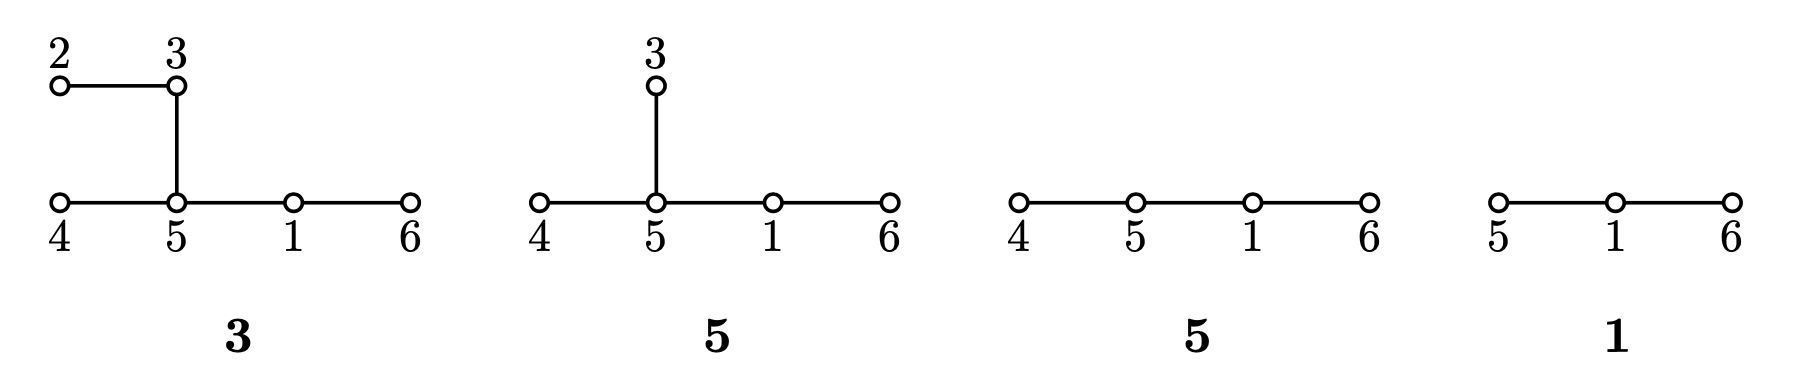
\includegraphics[width=0.7\linewidth]{Cayley.png}$$
Это правило определяет тотальную функцию из множества деревьев на множестве вершин $\{1, \ldots, n\}$ в последовательности длины $n-2$ из чисел, 
принадлежащих множеству $\{1, \ldots, n\}$. Докажем индукцией по числу вершин, что это биекция. Возникает проблема: после удаления 
вершины $m$ получается дерево, в котором вершины занумерованы не подряд

Чтобы избавиться от проблемы, усилим утверждение, которое будем доказывать. Будем доказывать существование биекции между деревьями, 
вершины которых принадлежат конечному множеству $V \subset \mathbb{N}$ и последовательностями длины $n-2$, элементы которых принадлежат $V$. Здесь $n=|V|$

База индукции: $n=2$. В этом случае последовательность пустая, её длина равна 0, а дерево единственное. Биекция между двумя 1-элементными множествами 
также единственная

Шаг индукции. Пусть уже доказано существование биекций указанного вида для любого $V$ с $|V|=n, n \geqslant 2$. Рассмотрим множество 
$V' \subset \mathbb{N}$, в котором $n+1$ число. Выполним один шаг построения последовательности Прюфера. То есть, найдём в дереве $T'$ 
с множеством вершин $V'$ висячую вершину $m$ с наименьшим номером

Соседа этой вершины обозначим $a$. Удалим $m$ из дерева. Получаем дерево на множестве вершин $V=V' \backslash\{m\}$. По предположению индукции 
есть биекция между деревьями на таком множестве вершин и $V^{n-2}$. Обозначим $\boldsymbol{x}_{T}$ последовательность, которая соответствует $T$. 
Тогда $T'$ сопоставляется последовательность $(a, \boldsymbol{x})$

Докажем, что получена биекция между деревьями с множеством вершин $V'$ и множеством последовательностей $\left(V'\right)^{n-1}$. 
Для этого построим обратную функцию. Пусть дана последовательность $\left(a, x_{1}, \ldots, x_{n-2}\right)$. Обозначим $m$ наименьшее число в множестве 
$V' \backslash\left\{a, x_{1}, \ldots, x_{n-2}\right\}$. Найдём дерево $T$ на множестве вершин $V=V' \backslash\{m\}$, соответствующее 
последовательности ($x_{1}, \ldots, x_{n-2}$) (по предположению индукции существует требуемая биекция, так как $m$ не входит в 
$\left\{x_{1}, \ldots, x_{n-2}\right\}$). Сопоставим последовательности $\left(a, x_{1}, \ldots, x_{n-2}\right)$ дерево $T'$, 
которое получается из $T$ добавлением висячей вершины $m$, соседней с $a$. Этому дереву мы и сопоставляем последовательность 
$\left(a, x_{1}, \ldots, x_{n-2}\right)$, значит построена обратная функция\qed



\subsection{Теорема о существовании монотонного остовного дерева}
\textbf{Формулировка.} В каждом связном графе существует монотонное остовное дерево\\[2mm]
\indent\textbf{Доказательство.} Выберем произвольную вершину $r$ связного графа $G$ в качестве корня. Построим нумерацию вершин графа, т.е. биекцию $\{1,2,\ldots,n\}\to V(G)$, $n=|V(G)|$, и корневой подграф $T$ с корнем $r$ следующим индуктивным процессом\\[2mm]
\indent Сопоставим корню число 1, $v_1=r$. После $i$ шагов получаем последовательность $v_1,\ldots,v_i$. Так как граф $G$ связный, то какие-то вершины из полученной последовательности смежны с вершинами из множетсва $V_i=V(G)\setminus\{v_1,\ldots,v_i\}$. На $(i+1)$-м шаге выберем среди всех ребер вида $\{v_j,u\},\ 1\leqslant j\leqslant i,\ u\in V_i$ то, для которого номер $j$ принимает наибольшее значение. Обозначим этот номер $k$. Если $j>k$, то $v_j$ смежна только с вершинами из уже построенной последовательности, а $v_k$ смежна с какими-то вершинами из $V_i$. Добавим в последовательность какого-нибудь непронумерованного соседа вершины $v_k$ и обозначим его $v_{i+1}$. Теперь добавляем ребро $\{v_k,v_{i+1}\}$ к ребрам $T$. Повторяем, пока $V_i\ne\varnothing$\\[2mm]
\indent Построенный граф $T$ связный: проверяем индукцией по номерам, что каждая вершина достижима из корня. В графе $T$ $(n-1)$ ребро, т.к. ровно одно ребро добавляется на каждом шаге, кроме первого. Значит, это дерево (согласно критерию—2 из \ref{1.4}). Теперь проверяем индукцией по номерам, что на каждом пути из корня в любую вершину номера строго возрастают\\[2mm]
\indent Докажем монотонность построенного остовного дерева от противного. Пусть $\{v_i,v_j\}$ — ребро графа $G,i<j$, и $v_i$ не лежит на пути из $v_j$ в $r=v_1$. Обозначим как $v_k$ вершину с максимальным номером, которая лежит выше и $v_i$, и $v_j$. Тогда из монотонности нумерации следует, что $k<i$. Расммотрим первую вершину на пути из $v_k$ в $v_j$, номер которой больше $i$ (такая вершина существует, т.к. $j>i$). Пусть ее номер равен $s$. На $(s-1)$-м шаге процесса выбрано ребро $\{v_t,v_s\}$ (причем $t<i$, т.к. $s$ — первая вершина на пути из $v_k$ в $v_j$ с номером, большим $i$), а не $\{v_i,v_j\}$, хотя $i>t,\ v_j\in V_{s-1}$, и вершина $v_i$ уже есть в построенной последовательности, т.к. $i<s$. Получаем противоречие с правилом построения последовательности $(v_1,\ldots,v_n)$\hfill$\square$

\subsection{Связь кликового числа и числа независимости для графа и его дополнения. Кликовое число и число независимости для полного графа. Кликовое число и число независимости для булева куба. Верхняя оценка на сумму кликового числа и числа независимости}
\subsubsection*{Связь кликового числа и числа независимости для графа и его дополнения}
Из определения понятно, что кликовое число графа $G$ равно числу независимости его дополнения, $\omega(G) = \alpha(\bar G)$, потому что рёбра и нерёбра меняются местами при переходе к дополнению
\subsubsection*{Кликовое число и число независимости для полного графа}
Для полного графа из определений получаем $\omega(K_n) = n$, а $\alpha(K_n) = 1$
\subsubsection*{Кликовое число и число независимости для булева куба}
Обозначим через $I_0$ множество вершин булева куба $Q_n$ (двоичных слов длины $n$), в которых чётное количество единиц, а через $I_1$ — множество вершин булева куба $Q_n$, в которых нечётное количество единиц\\[2mm]
\indentПри инвертировании одной позиции количество единиц в слове изменяется ровно на 1. Поэтому концами каждого ребра являются слова, у которых чётность количества единиц разная — в одном количество единиц чётно, в другом — нечётно. Значит, между вершинами из $I_0$ рёбер нет (как и между вершинами из $I_1$). Из свойств биномиальных коэффициентов мы знаем, что $\left|I_0\right|=\left|I_1\right|$. Таким образом $\alpha\left(Q_n\right) \geqslant 2^{n-1}$ (половина всех вершин)\\[2mm]
\indent Докажем, что в булевом кубе $Q_n$ нет независимого множества размера больше $2^{n-1}$\\[2mm]
\indentПусть $I$ — независимое множество. Степень любой вершины в булевом кубе $Q_n$ равна $n$. Поэтому количество рёбер, инцидентных $I$, равно $n|I|$. Это число не больше общего количества рёбер $n 2^{n-1}$. Отсюда получаем неравенство $|I| \leqslant 2^{n-1}$. Итак, $\alpha\left(Q_n\right)=2^{n-1}$\\[2mm]
\indentКлика размера 2 — это ребро и такие клики есть в $Q_n$ при $n>0$. Клика размера 3 — треугольник — в $Q_n$ невозможна. Из любых трёх вершин две лежат в одном из множеств $I_0, I_1$ (имеют одинаковую чётность количества единиц) и потому не связаны ребром. Поэтому $\omega\left(Q_n\right)=2$
\subsubsection*{Верхняя оценка на сумму кликового числа и числа независимости}
Любая клика пересекает любое независимое множество разве что по одной вершине, поэтому $\alpha(G)+\omega(G)\leqslant n+1$ для любого графа $G$. Оценка достигается, например, на полном графе


\subsection{Теорема Рамсея}
\textbf{Формулировка.} Для любых $k,n$ найдется такое число $N_0$, что в любом графе на $N\geqslant N_0$ вершинах есть клика размера $k$ или независимое множество размера $n$\\[2mm]
\indent\textit{Disclaimer.} Теорема Рамсея говорит лишь о существовагнии чисел Рамсея, а мы докажем верхнюю оценку на них: $$R(k,n)\leqslant R(k-1,n)+R(k,n-1),\ k>1,n>1$$ и сам факт существования чисел Рамсея\\[2mm]
\indent\textbf{Доказательство.} Пусть $k+n=s$. Докажем индукцией по $s$\\[2mm]
\indent База $s=2$ очевидна: $2=1+1$\footnote{Так как это единственный способ разложить число 2 на сумму двух положительных чисел}\\[2mm]
\indentШаг индукции. Предположим, что неравенство (верхняя оценка) выполняется для всех пар $(k,n)$ таких, что $k+n=s$\\[2mm]
\indent Докажем неравенство для такой пары $(k,n)$, что $k+n=s+1,\ k>1,n>1$. Согласно индуктивному предположению существуют числа Рамсея $R(k-1,n)$ и $R(k,n-1)$\\[2mm]
\indent Рассмотрим граф на $N_0=R(k-1, n)+R(k, n-1)$ вершинах и выберем произвольную вершину $v$ этого графа. Вершин в графе за исключением вершины $v$ ровно $N_0-1$ штук. Среди них $N_1$ соседей и $N_2$ несоседей вершины $v$\\[2mm]
\indent Докажем, что выполняется хотя бы одно из неравенств от противного
$$\begin{aligned}
& N_1 \geqslant R(k-1, n), \\
& N_2 \geqslant R(k, n-1) .
\end{aligned}$$
\indentДействительно, в противном случае выполняются два неравенства
$$\begin{aligned}
& N_1<R(k-1, n), \\
& N_2<R(k, n-1),
\end{aligned}$$
из которых следует противоречие $$N_0-1=N_1+N_2 \leqslant R(k-1, n)-1+R(k, n-1)-1=N_0-2$$
\indent Поэтому у вершины $v$ есть хотя бы $R(k-1, n)$ соседей или есть хотя бы $R(k, n-1)$ несоседей. Рассмотрим случаи\\[2mm]
\indent\textit{Первый случай.} В индуцированном соседями вершины $v$ подграфе по предположению индукции найдётся клика размера $k-1$ или независимое множество размера $n$. В первом варианте добавление вершины $v$ даёт клику в исходном графе размера $k$, во втором варианте в исходном графе есть независимое множество размера $n$\\[2mm]
\indent\textit{Второй случай.} В индуцированном несоседями вершины $v$ подграфе по предположению индукции найдётся клика размера $k$ или независимое множество размера $n-1$. В первом варианте в исходном графе есть клика размера $k$, а во втором добавление вершины $v$ даёт независимое множество размера $n$ в исходном графе\\[2mm]
\indent Мы доказали, что для $k+n=s+1$ теорема Рамсея выполняется, как и неравенство верхней оценки. Значит, для всех $k, n$ теорема Рамсея верна и при $k>1, n>1$ выполняется неравенство верхней оценки по принципу математической индукции\hfill$\square$
\label{2.9}

\subsection{Верхняя оценка на числа Рамсея. Явные выражения для \texorpdfstring{$R(2,n)$}{R(2,n)} и \texorpdfstring{$R(3,3)$}{R(3,3)}}
\textbf{Верхняя оценка на числа Рамсея}. $R(k,n)\leqslant\begin{pmatrix}
    k+n-2\\
    k-1
\end{pmatrix}$\\[2mm]
\indent\textbf{Доказательство.} Для биномиальных коэффициентов выполняется $$\begin{pmatrix}
    k+n\\
    k
\end{pmatrix}=\begin{pmatrix}
    k+n-1\\
    k-1
\end{pmatrix}+\begin{pmatrix}
    k+n-1\\
    k
\end{pmatrix}$$
\indent Заметим, что $R(k,1)=R(1,n)$, т.к. одна вершина является и кликой, и незаивсимым множеством. Искомое неравенство справедливо при $k=1$ или $n=1$, т.к. $R(k,1)=R(1,n)=\binom{n-1}{0}$\\[2mm]
\indent Для остальных случаев докажем индукцией по $k+n=s$. База доказана ранее. Проверим шаг индукции при $k>1,n>1$ с помощью неравенства из \ref{2.9}: $$R(k,n)\leqslant R(k-1,n)+R(k,n-1)\leqslant\begin{pmatrix}
    k+n-3\\
    k-2
\end{pmatrix}+\begin{pmatrix}
    k+n-3\\
    k-1
\end{pmatrix}=\begin{pmatrix}
    k+n-2\\
    k-1
\end{pmatrix}$$
Во втором неравенстве использовалось индуктивное предположение\hfill$\square$\\[4mm]
\indent\textbf{Явное выражение—1.} $R(2,n)=\dbinom{n}{1}=n$\\[2mm]
\indent\textbf{Доказательство.} Если в графе $G$ есть хотя бы одно ребро, то $\omega(G)\geqslant2$. Если ребер нет, тогда $\alpha(G)=|V(G)|$. Значит, если в графе есть хотя бы $n$ вершин, то в нём есть либо ребро и, тем самым, клика размера 2, либо в нём нет рёбер и есть независимое множество размера $n$. Если в графе нет рёбер и вершин меньше $n$, в нём нет ни клики размера 2, ни независимого множества размера $n$\hfill$\square$\\[4mm]
\indent\textbf{Явное выражение—2.} $R(3,3)=\dbinom{4}{2}=6$\\[2mm]
\indent\textbf{Доказательство.} Докажем, что $R(3,3)\leqslant
6$. Это частный случай верхней оценки числа Рамсея: $R(3,3)\leqslant\dbinom{3+3-2}{3-1}=6$\\[2mm]
\indent Чтобы доказать $R(3, 3) > 5,$ приведем пример графа на 5 вершинах, в котором нет треугольника (клики размера 3) и в дополнении к которому нет треугольника. Таким графом является цикл $C_5$. Что в нём нет клики размера 3, очевидно из построения. А дополнение к $C_5$ также является циклом на 5 вершинах. Так что независимого множество размера 3 в нём также нет\hfill$\square$

\subsection{Уточнение верхней оценки на числа Рамсея}
\textbf{Формулировка.} Если оба числа $R(k-1,n),R(k,n-1)$ четные, то $$R(k,n)\leqslant R(k-1,n)+R(k,n-1)-1$$
\indent\textbf{Доказательство.} Пусть $R(k-1,n),\ R(k,n-1)$ четные. Рассмотрим граф на $N_0=R(k-1,n)+R(k,n-1)-1$ вершинах. Это число нечетное, поэтому в графе есть вершина $v$ четной степени, т.к. сумма степеней вершин четная\\[2mm]
\indentВершин в графе за исключением $v$ ровно $N_0-1$ штук. Среди них $N_1$ соседей и $N_2$ несоседей вершины $v$ и оба числа чётные, так как $N_1$ чётное по выбору вершины $v$ и $N_1+N_2=N_0-1$ чётное\\[2mm]
\indentДокажем, что выполняется хотя бы одно из неравенств
$$\begin{aligned}
& N_1 \geqslant R(k-1, n), \\
& N_2 \geqslant R(k, n-1) .
\end{aligned}$$
\indentВ противном случае выполняются два неравенства
$$\begin{aligned}
& N_1<R(k-1, n), \quad \text { что равносильно } N_1 \leqslant R(k-1, n)-2, \\
& N_2<R(k, n-1), \quad \text { что равносильно } N_2 \leqslant R(k, n-1)-2 .
\end{aligned}$$
\indentПолучаем противоречие
$$N_0-1=N_1+N_2 \leqslant R(k-1, n)-2+R(k, n-1)-2=N_0-3$$
\indent Поэтому у вершины $v$ есть хотя бы $R(k-1, n)$ соседей или есть хотя бы $R(k, n-1)$ несоседей. Рассмотрим случаи\\[2mm]
\indent Далее также рассматриваем случаи, как в \ref{2.9}\hfill$\square$

\subsection{Нижняя оценка на числа Рамсея}
\textbf{Формулировка.} $R(k,k)>\lfloor 2^{(k-1)/2}\rfloor\ \forall k\geqslant3$\\[2mm]
\indent \textit{Другими словами}, $\forall k\geqslant3$ существует граф $G=(V,E)$ на $n=\lfloor2^{(k-1)/2}\rfloor$ вершинах, в котором нет ни клики размера $k$, ни независимого множества размера $k$\\[2mm]
\indent\textbf{Доказательство.} Оценим количество графов на $n$ вершинах, содержащих либо клику размера $k$, либо независимое 
множество такого размера, и сравним это число с общим количеством графов. При больших $n$ первое число намного меньше второго. Это и означает, что 
существуют графы на $n$ вершинах без клик и без независимых множеств размера $k$

Множество графов на $n$ вершинах находится во взаимно однозначном соответствии с подмножествами множества 
пар вершин (каждое ребро или проведено, или нет). Всего пар вершин (=рёбер) $\binom{n}{2}$, 
поэтому графов $2\binom{n}{2}$

Обозначим через $A$ множество графов, содержащих клику или независимое множество размера $k$. Это множество является объединением множеств $A_{W}$, 
где $W \subseteq V$, 
$|W|=k$, которые состоят из тех графов, в которых множество $W$ образует клику или независимое множество. Запишем это формально

$$
A=\bigcup_{\substack{W \subseteq V,\\|W|=k}} A_{W}
$$

Воспользуемся оценкой объединения: для любого семейства конечных подмножеств $X_{1}, \ldots, X_{t}$ выполняется

$$
\left|\bigcup_{i} X_{i}\right| \leqslant \sum_{i}\left|X_{i}\right|
$$

Оценка объединения — упрощённый вариант формулы включений и исключений. Пересчитывая все элементы во всех множествах, 
получаем правую часть, при этом все элементы будут пересчитаны и, возможно, даже не по одному разу

Итак,

$$
|A| \leqslant \sum_{\substack{W \subseteq V \\|W|=k}}\left|A_{W}\right|
$$

Посчитать количество графов в $A_{W}$ легко. Ребра между вершинами в $W$ в таком графе должны либо все присутствовать, либо все отсутствовать. 
Ребра, хотя бы один конец которых лежит вне $W$, могут быть произвольными. Количество рёбер, у которых хотя бы один конец лежит вне $W$, есть 
$\binom{n}{2}-\binom{k}{2}$ (все ребра минус ребра в $W$). Таким образом, 
количество таких графов есть $2 \cdot 2^{\binom{n}{2}-\binom{k}{2}}$, 
где первая двойка отвечает за выбор рёбер внутри $W$, а второй множитель — за выбор остальных рёбер. То есть

$$
\left|A_{W}\right|=2^{\binom{n}{2}-\binom{k}{2}+1}
$$

Таким образом, при $k \geqslant 3, n=\left\lfloor 2^{(k-1) / 2}\right\rfloor$ получаем неравенство

$$
\begin{aligned}
\frac{|A|}{2^{\binom{n}{2}}} & \leqslant \sum_{\substack{W \subseteq V,\\|W|=k}} 2^{-\binom{k}{2}+1}=\binom{n}{k} \cdot 2^{-\binom{k}{2}+1}=
\frac{n(n-1) \cdots(n-k+1)}{k !} \cdot 2^{-\binom{k}{2}+1} \leqslant \\
& \leqslant \frac{n^{k}}{2 \times 3} \cdot 2^{-\binom{k}{2}+1} \leqslant \frac{2^{k(k-1) / 2-\binom{k}{2}+1}}{6}=\frac{1}{3}
\end{aligned}
$$

Поэтому количество графов с кликой или независимым множеством размера $k$ не более трети от общего числа графов. 
Значит, не менее двух третей графов с таким количеством вершин удовлетворяют условию теоремы\qed


\subsection{Критерий 1-раскрашиваемости графа. Критерий 2-раскрашиваемости графа. 2 - раскрашиваемость булева куба}
\subsubsection*{Критерий 1-раскрашиваемости графа}
\textbf{Формулировка.} Все \textbf{графы без ребер} 1-раскрашиваемые\\[2mm]
\indent\textbf{Доказательство.} Если вершинам графа без рёбер присвоить число 1, то условие правильной раскраски выполняется. И наоборот: если в графе есть ребро $\{u, v\}$, то в правильной раскраске вершинам $u$, $v$ присвоены разные цвета, поэтому количество цветов хотя бы 2\hfill$\square$
\subsubsection*{Критерий 2-раскрашиваемости графа}
\textbf{Формулировка.} 2-раскрашиваемые графы это в точности графы, в которых длины всех циклов чётные\\[2mm]
\indent\textbf{Доказательство.} Если вершины графа правильно раскрашены в 2 цвета, то цвета вершин вдоль любого пути чередуются, т.к. соседние вершины покрашены в разные цвета. Поэтому длина любого цикла в таком графе чётная (концы пути нечётной длины покрашены в разные цвета)\\[2mm]
\indent Докажем обратное. Достаточно доказать утверждение для связных графов, т.к. несвязный граф 2-раскрашиваемый тогда и только тогда, когда все его компоненты связности 2-раскрашиваемые и то же самое верно для свойства «длины всех циклов чётные»\\[2mm]
\indentПусть в связном графе длины всех циклов чётные. Докажем, что для любых двух вершин $u,\ v$ в этом графе длины путей из $u$ в $v$ имеют одинаковую чётность\\[2mm]
\indent Если в графе есть путь $\alpha=(u,\ldots,v)$ с четным числом вершин (нечетной длины), а также другой путь $\beta=(u,\ldots,v)$ с нечетным числом вершин (четной длины), то соединение пути $\alpha$ и обратного к $\beta$ пути, т.е. пути $(v,\ldots,u)$, даёт цикл с нечётным числом вершин (нечётной длины). Это противоречит сделанному предположению, что все циклы в графе имеют чётную длину\\[2mm]
\indent Теперь укажем искомую правильную раскраску в 2 цвета. Выберем вершину $v_0$ и раскрасим вершину $x$ графа в цвет 0, если длины путей из $v_0$ в $x$ чётные, и в цвет 1 — если иначе. Это правило корректно по доказанному выше утверждению про одинаковую чётность длин путей с общими концами в связном графе, все циклы которого чётные\\[2mm]
\indentПри такой раскраске смежные в графе вершины не могут быть покрашены в один цвет:  если $\{x,y\}$ — ребро графа, то для пути $(v_0,\ldots,x)$ существует путь в $y$, длина которого имеет противоположную четность: $(v_0,\ldots,x,y)$\hfill$\square$

\subsubsection*{2-раскрашиваемость булева куба}
\textbf{Формулировка.} Булев куб $Q_n$ 2-раскрашиваемый\\[2mm]
\indent\textbf{Доказательство.} Вершинами булева куба $Q_n$ являются двоичные слова длины $n$. Покрасим вершины с чётным количеством единиц в цвет 0; с нечётным количеством единиц — 1\\[2mm]
\indentРебро булева куба связывает вершины, которые отличаются ровно в одной позиции. Одна вершина на этой позиции содержит 0, другая — 1. Чётность количества единиц в таких вершинах разная, то есть они покрашены в разные цвета\hfill$\square$

\subsection{Количество совершенных паросочетаний в полном графе на \texorpdfstring{$2n$}{2n} вершинах}
\textbf{Формулировка.} Количество совершенных паросочетаний в полном графе на $2n$ вершинах равно $(2n-1)!!$\footnote{Двойной факториал $n!!$ означает произведение членов в арифметической прогрессии с началом $n$ и разностью равной —2}\\[2mm]
\indent\textbf{Доказательство.} Определим функцию $f:S_{2n}\to\Pi_{2n}$, где $S_{2n}$ — перестановки чисел от 1 до $2n$, а $\Pi_{2n}$ — совершенные паросочетания в полном графе на множетсве вершин $\{1,2,\ldots,2n\}$. Перестановку $x_1x_2\ldots x_{2n}$ функция отправляет в паросочетание $$\{\{x_1,x_2\},\{x_3,x_4\},\ldots,\{x_{2n-1},x_{2n}\}\}$$
\indent Из определения понятно, что функция тотальная. Определим размер прообраза одного паросочетания. Паросочетание не изменится, если поменять местами $x_{2 i+1}$ и $x_{2 i}$ для любого $0 \leqslant i \leqslant n-1$, а также если переставить все такие $n$ пар произвольным образом. В любом другом случае паросочетание изменяется. По правилу произведения размер прообраза любого паросочетания равен ($2!)^nn!$. Получаем равенство $$(2n)!=(2!)^n n!P_{2 n},$$
из которого выводим искомую формулу для количества совершенных паросочетаний:
$$P_{2 n}=\frac{(2 n) !}{(2 !)^n n !}=\frac{2 n \cdot(2 n-1) \cdot \ldots \cdot 2 \cdot 1}{2 n \cdot(2 n-2) \cdot \ldots \cdot 2}=(2 n-1) \cdot(2 n-3) \cdot\ldots \cdot 1=(2 n-1) ! !$$\qed


\subsection{Теорема Холла}
\textbf{Формулировка.} $G=(L,R,E)$ — двудольный граф. Тогда в графе $G$ есть паросочетаание размера $|L|$ тогда и только тогда, когда для каждого множества $S\subseteq L$ множество соседей $G(S)\subseteq R$ содержит не меньше вершин, чем $S$\\[2mm]
\indent\textbf{Доказательство.} Если есть паросочетание размера $|L|$, то условие Холла выполняется: у каждого $S\subseteq L$ соседей не меньше, чем $|S|$ (в эти соседи входят концы в правой доле каждого ребра паросочетания, инцидентного вершине из $S$)\\[2mm]
\indent В другую сторону докажем с помощью полной индукции по количеству элементов в $L$\\[2mm]
\indent \textbf{База индукции.} Если в $L$ всего одна вершина $x$, тогда у нее есть хотя бы один сосед $y$ в правой доле $R$ (по условию теоремы). Получаем паросочетание с ребром  $\{x,y\}$\\[2mm]
\indent\textbf{Шаг индукции.} Предположим, что утверждение теоремы выполняется для всех двудольных графов, в которых левая доля содержит меньше $n$ вершин. Рассмотрим граф $G=(L, R, E)$, для которого выполняются условия теоремы и в $L$ ровно $n$ вершин. Разберём два случая:\\[2mm]
\indent \textit{Первый случай:} в левой доле есть такое множество $\varnothing \neq S \subset L$, для которого $|S|=|G(S)|$\\[2mm]
\indent Выделим из графа два подграфа. Первый, $G'$, имеет доли $S,\ G(S)$ и все рёбра графа $G$ между этими вершинами. Второй, $G''$, имеет доли $T=L\setminus S$, $Q=R \setminus G(S)$ и все рёбра графа $G$ между этими вершинами. Для обоих графов выполняются условия теоремы Холла. Для $G'$ это выполняется, так как множество соседей подмножества $X \subseteq S$ лежит в $G(S)$\\[2mm]
\indentТеперь проверим условие Холла для графа $G''$, то есть $\left|G''(X)\right| \geqslant|X|$ для любого подмножества $X \subseteq T$. Заметим, что $G(S \cup X)=G(S) \cup G''(X), S \cap X=\varnothing$, $G(S) \cap G''(X)=\varnothing$ по построению графа $G''$. Из условия Холла для графа $G$ и выбора множества $S$ получаем $$|G(S \cup X)|=|G(S)|+\left|G''(X)\right|=|S|+\left|G''(X)\right| \geqslant|S \cup X|=|S|+|X|$$
Отсюда следует искомое неравенство $\left|G''(X)\right| \geqslant|X|$\\[2mm]
\indent Поскольку для $G', G''$ выполняются условия Холла, а количество вершин в этих графах меньше $n$, то по предположению индукции в каждом из этих графов есть паросочетание размера левой доли. Объединяя эти два паросочетания, получаем искомое паросочетание в $G$ размера $|L|$\\[2mm]
\indent \textit{Второй случай:} для каждого $\varnothing \neq S \subset L$ выполняется неравенство $|S|<|G(S)|$\\[2mm]
\indentВыберем вершину $a \in L$ и её соседа $b \in R$ (в этом случае соседей у каждой вершины больше одного)\\[2mm]
\indent Проверим, что для графа $G'=\left((L \setminus\{a\}),(R \setminus\{b\}), E'\right)$, полученного из $G$ выбрасыванием вершин $a, b$ и инцидентных им рёбер, выполняются условия Холла. Количество соседей множества $X \subseteq L \setminus\{a\}$ в графе $G'$ разве что на 1 меньше, чем в графе $G$ (различие только в вершине $b$). Так как $|X|<|G(X)|$, то $|X| \leqslant\left|G'(X)\right|$\\[2mm]
\indent Значит, по индуктивному предположению, в графе $G'$ существует паросочетание размера $n-1$. Добавим к рёбрам этого паросочетания ребро $\{a, b\}$. Тогда получим паросочетание размера $n$ в графе $G$  \qed

\subsection{Следствия из теоремы Холла для регулярных двудольных графов}
\textbf{Следствие—1.} В регулярном двудольном графе, степени вершин которого ненулевые, существует совершенное паросочетание\\[2mm]
\indent\textbf{Доказательство.} Пусть степень каждой вершины в регулярном двудольном графе $G=(L, R, E)$ равна $d$, по условию $d \neq 0$. Заметим, что тогда $|E|=d|L|=d|R|$, то есть $|L|=|R|$. Докажем, что условие теоремы Холла выполняется (и потому существует паросочетание размера $L$, которое является совершенным)\\[2mm]
\indentРассмотрим множество $S \subseteq L$ вершин левой доли. Эти вершины являются концами $d|S|$ рёбер. По определнию $G(S)$ — концы этих ребер в правой доле. Подсчитывая рёбра между $S$ и $G(S)$ двумя способами, получаем $d|S| \leqslant d|G(S)|$. Первое число — подсчёт рёбер по левым концам. Второе — по правым (каждая из этих вершин является концом не более, чем $d$ рёбер, ведущих в $S$, поскольку степень вершины равна $d$). Значит, теорема Холла выполняется\qed\\[2mm]
\indent\textbf{Следствие—2.} Если степень каждой вершины в двудольном графе равна $d > 0,$ то его рёбра можно разбить на $d$ непересекающихся совершенных паросочетаний\\[2mm]
\indent\textbf{Доказательство.} Индукция по степени вершин в графе $d$\\[2mm]
\indentБаза очевидна: $d=1$, такой граф и есть совершенное паросочетание\\[2mm]
\indent Шаг индукции: применим следствие—1 и выделим рёбра полученного совершенного паросочетания. Остальные рёбра образуют регулярный граф степени $d-1$, который разбивается на $d-1$ совершенное паросочетание по индуктивному предположению\qed

\subsection{Связь между вершинными покрытиями и независимыми множествами. Связь минимального размера вершинного покрытия с числом независимости. Связь минимального размера вершинного покрытия с максимальным размером паросочетания. Пример, показывающий возможность строгого неравенства из последнего утверждения}
\subsubsection*{Связь между вершинными покрытиями и независимыми множествами}
\textbf{Формулировка.} Множество $S$ вершин графа $G=(V,E)$ является вершинным покрытием тогда и только тогда, когда $V\setminus S$ — независимое множество\\[2mm]
\indent\textbf{Доказательство.} Пусть $S$ — вершинное покрытие. Тогда у каждого ребра хотя бы один из концов лежит в $S$. Поэтому рёбер между вершинами из $V\setminus S$ нет.
Пусть $V\setminus S$ — независимое множество. Тогда у каждого ребра хотя бы один из концов лежит вне этого множества\\
\indentЗначит, $S$ — вершинное покрытие\qed
\subsubsection*{Связь минимального размера вершинного покрытия с числом независимости}
\textbf{Формулировка.} Минимальный размер вершинного покрытия в графе $G$: $\tau(G)=n-\alpha(G)$, где $n$ — количество вершин в графе, $\alpha(G)$ — число независимости\\[2mm]
\indent\textbf{Доказательство.} тут ачев, следует из связи между вершинными покрытиями и независимыми множествами\qed
\subsubsection*{Связь минимального размера вершинного покрытия с максимальным размером паросочетания}
\noindentМаксимальный размер паросочетания — $\mu(G)$\\[2mm]
\indent\textbf{Формулировка.} $\tau(G)\geqslant\mu(G)$ для любого графа $G$\\[2mm]
\indent\textbf{Доказательство.} Если $P$ — паросочетание, то любое вершинное покрытие содержит хотя бы по одному концу каждого ребра паросочетания, а следовательно его размер не меньше размера паросочетания\qed
\label{2.17}
\subsubsection*{Пример}
В графе-цикле $C_5$ никакие две вершины не покрывают все рёбра цикла $C_5$, но, тремя вершинами рёбра покрываются, значит $\tau(C_5) = 3$. Так как в паросочетании из трёх рёбер должно быть 6 вершин, то $\mu(C_5) = 2$, при этом паросочетание размера 2 легко находится\qed

\subsection{Теорема Кёнига}
\textbf{Формулировка.} В любом двудольном графе $G$ выполняется равенство $\tau(G) = \mu(G)$\\[2mm]
\indent\textbf{Доказательство.} Неравенство  $\tau(G)\geqslant\mu(G)$ доказано в \ref{2.17}. Докажем  $\tau(G)\leqslant\mu(G)$ для двудольных графов с помощью теоремы Холла\\
\indent В двудольном графе $G=(L, R, E)$ рассмотрим минимальное по размеру вершинное покрытие $X \cup Y, X \subseteq L, Y \subseteq R$. Определим два подграфа: $G'=$ $\left(X, G(X) \setminus Y ; E'\right), G''=\left(Y, G(Y) \setminus X ; E''\right)$\\[2mm]
\indentПроверим, что для этих графов выполняется условие Холла. Рассуждения для обоих графов аналогичны, приведём их для $G'$. Пусть $S \subseteq X$. Множество $(X \setminus S)\ \cup$ $Y \cup G'(S)$ является вершинным покрытием в $G$ : все рёбра, покрытые вершинами из $S$, покрыты также либо вершинами из $Y$, либо соседями вершин $S$ в правой доле. Поскольку мы выбрали минимальное по размеру вершинное покрытие, $\left|G'(S)\right| \geqslant|S|$, что и означает выполнение условия Холла\\[2mm]
\indentПо теореме Холла в $G'$ есть паросочетание размера $|X|$, а в $G''$ есть паросочетание размера $|Y|$. Рёбра этих паросочетаний не совпадают по построению. Значит, объединение этих паросочетаний даёт паросочетание размера $|X|+|Y|$ в графе $G$. Таким образом, размер максимального паросочетания в $G$ не меньше размера минимального вершинного покрытия\qed


\subsection{Лемма про сумму исходящих и входящих степеней вершин. Свойства отношения достижимости в орграфе. Свойства отношения сильной связанности в орграфе}
\subsubsection*{Лемма}
\textbf{Формулировка.} Сумма исходящих степеней всех вершин равна сумме входящих степеней всех вершин: обе суммы равны числу рёбер графа\\[2mm]
\indent\textbf{Доказательство.} Каждое ребро имеет одно начало (выходит из какой-то вершины) и поэтому учитывается по одному разу, когда мы складываем исходящие степени всех вершин. Аналогично для концов рёбер\qed

\subsubsection*{Свойства отношения достижимости в орграфе}
\textbf{Формулировка.} Свойства любого простого ориентированного графа и любых его вершин $v_1$, $v_2$, $v_3$:\\[2mm]
\indent 1. \textit{рефлексивность:} $(v,v)\in R$ — вершина достижима из самой себя\\[2mm]
\indent 2. \textit{транзитивность:} если $(v_1,v_2)\in R$ и $(v_2,v_3)\in R$, то $(v_1,v_3)\in R$\\[2mm]
\indent\textbf{Доказательство.} Так как $v$ — путь (длины 0), вершина $v$ связанная с самой собой\\[2mm]
\indent Если в графе есть пути $v_{1} u_{1} \ldots u_{s} v_{2}$ и $v_{2} w_{1} \ldots w_{t} v_{3}$ (то есть $\left(v_{1}, v_{2}\right) \in R$ и $\left.\left(v_{2}, v_{3}\right) \in R\right)$, то в этом графе есть также и путь $v_{1} u_{1} \ldots u_{s} v_{2} w_{1} \ldots w_{t} v_{3}$, то есть $\left(v_{1}, v_{3}\right) \in R$. Значит, вершина $v_{3}$ достижима из $v_{1}$\qed
\label{2.19}

\subsubsection*{Свойства отношения сильной связанности в орграфе}
\textbf{Форулировка.} Для любого ориентированного графа отношение сильной связанности \textit{рефлексивно, симметрично и транзитивно}, то есть является отношением эквивалентности\\[2mm]
\indent\textbf{Доказательство.}\\[2mm]
\indent\textit{Рефлексивность:} $v_1$ — путь в любом графе, поэтому $v_1$ сильно связана сама с собой\\[2mm]
\indent\textit{Транзитивность:} если в графе есть пути из $v_1$ в $v_2$, из $v_2$ в $v_1$, из $v_2$ в $v_3$, из $v_3$ в $v_2$, то обязательно есть и пути из $v_1$ в $v_3$ (соединяем путь из $v_1$ в $v_2$ с путём из $v_2$ в $v_3$), а также из $v_3$ в $v_1$ (соединяем путь из $v_3$ в $v_2$ с путём из $v_2$ в $v_1$)\\[2mm]
\indent\textit{Симметричность:} если $(u, v) \in C$, то по определению $(u, v) \in R$ и $(v, u) \in R$. Отсюда следует, что и $(v, u) \in C$\qed

\subsection{Критерий эйлеровости ориентированного и неоринтированного графа}
\subsubsection*{Критерий—1}
\textbf{Формулировка.} В ориентированном графе без изолированных вершин существует эйлеров цикл тогда и только тогда, когда граф сильно связен и у любой вершины входящая степень равна исходящей\\[2mm]
\indent\textbf{Доказательство.} Пусть эйлеров цикл в орграфе есть. Тогда он проходит через все вершины (поскольку они имеют ненулевую степень), и по нему можно дойти от любой вершины до любой. Значит, орграф сильно связен\\[2mm]
\indentВозьмём какую-то вершину $v$, пусть она встречается в эйлеровом цикле $k$ раз. Двигаясь по циклу, мы приходим в неё $k$ раз и уходим $k$ раз, значит, использовали $k$ входящих и $k$ исходящих рёбер. При этом, раз цикл эйлеров, других рёбер у этой вершины нет, так что в ориентированном графе её входящая и исходящая степени равны $k$\\[2mm]
\indentВ обратную сторону. Пусть орграф сильно связен и в каждой вершине исходящая степень равна входящей. Выберем самый длинный простой в рёбрах путь, т.е. его длина не больше общего количества рёбер
$$\tau=\left(v_0, v_1, v_2, \ldots, v_{t-1}, v_t\right)$$
и докажем, что этот путь и является искомым циклом, то есть что $v_0=v_t$ и этот путь содержит все рёбра орграфа\\[2mm]
\indent Если $\tau$ самый длинный, то добавить к нему ребро $\left(v_t, v_{t+1}\right)$ невозможно. Значит, что все выходящие из $v_t$ рёбра уже входят в $\tau$. Это возможно, лишь если $v_0=v_t$ : если вершина $v_t$ встречалась только внутри пути (пусть она входит $k$ раз внутри пути и ещё раз в конце пути), то мы использовали $k+1$ входящих рёбер и $k$ выходящих, и больше выходящих нет. Это противоречит равенству входящей и исходящей степени\\[2mm]
\indentИтак, мы имеем цикл, и осталось доказать, что в него входят все рёбра. Пусть из какой-то вершины $v_i$ выходит ребро $\left(v_i, v\right)$, не входящее в выбранный путь (цикл на самом деле). Тогда этот путь можно удлинить до простого в рёбрах пути
$$\left(v_{i+1}, \ldots, v_t=v_0, \ldots, v_i, v\right)$$
вопреки нашему выбору (самого длинного простого в рёбрах пути). Аналогично можно получить противоречие и для входящего ребра $\left(v, v_i\right)$, добавив его в начало\\[2mm]
\indentЗначит, во всех вершинах цикла использованы все инцидентные им рёбра. Но орграф сильно связен, поэтому выбранный цикл содержит все рёбра этого графа и проходит через все вершины\qed

\subsubsection*{Критерий—2}
\textbf{Формулировка.} Неориентированный граф без вершин нулевой степени содержит эйлеров цикл тогда и только тогда, когда он связен и степени всех вершин чётны\\[2mm]
\indent\textbf{Доказательство аналогично критерию—1.} Пусть эйлеров цикл в графе есть. Он проходит по всем вершинам, значит граф связен. В каждую вершину эйлеров цикл $k$ раз заходит и $k$ раз выходит. Значит, степень вершины $k + k = 2$k чётна\\[2mm]
\indentВ обратную сторону опять рассматриваем самый длинный путь, в котором каждое ребро встречается не больше одного раза. Это цикл, т.к. иначе есть вершина нечётной степени\\
\indentЭтот цикл обязан содержать все рёбра графа, т.к. в противном случае его можно удлинить\qed

\subsection{Лемма о существовании в ациклическом графе вершины с исходящей степенью 0 и вершины с входящей степенью 0. Равносильные определения ациклического графа}
\subsubsection*{Лемма}
\textbf{Формулировка.} В ациклическом орграфе есть вершина, из которой не выходит ни одного ребра, а также есть вершина, в которую не входит ни одно ребро\\[2mm]
\indent\textbf{Доказательство.} Выберем в этом орграфе простой путь максимальной длины, обозначим его вершины $v_0, v_1, \ldots, v_t$. Тогда исходящая степень вершины $v_t$ равна 0: если в орграфе есть ребро $\left(v_t, x\right), x \notin\left\{v_0, \ldots, v_{t-1}\right\}$, то длина выбранного пути не максимальна: его можно продолжить до пути $v_0, \ldots, v_t, x$. Если же в орграфе есть ребро $\left(v_t, v_i\right)$, то в этом орграфе есть цикл $v_i, \ldots, v_t, v_i$\\[2mm]
\indentАналогично доказывается, что входящая степень вершины $v_0$ равна 0\qed
\label{2.21}

\subsubsection*{Равносильные определения ациклического графа}
\textbf{Формулировка.} Следующие свойства орграфа без петель равносильны:\\[2mm]
\indent 1. Каждая компонента сильной связности состоит из одной вершины\\[2mm]
\indent 2. Орграф ациклический\\[2mm]
\indent3. Вершины орграфа можно пронумеровать натуральными числами таким образом, чтобы все рёбра вели из вершины c меньшим номером в вершину с б\'oльшим\\[2mm]
\indent\textbf{Доказательство.} Доказываем утверждения теоремы по очереди\\[2mm]
\textit{Доказательство} (1)$\implies(2)$. Равносильно контрапозиции $\neg(2)\implies\neg(1)$. Раз в орграфе нет петель, в нём нет циклов длины 1. Если в орграфе есть цикл с $n > 1$ вершинами, то вершины этого цикла сильно связаны (из любой можно попасть в любую по циклу) — и тогда они попадут в одну компоненту связности\\[3mm]
\textit{Доказательство $(2)\implies(1)$}. Равносильно контрапозиции $\neg(1)\implies\neg(2)$. Если вершины $a\ne b$ сильно связаны, то существуют пути из $a$ в $b$ и из $b$ в $a$. Соединением этих путей получается цикл длины $> 0$\\[3mm]
\textit{Докзательство $(3)\implies(2)$}. Если возможна нумерация вершин, при которой все рёбра идут из меньшей вершины в б\'oльшую, то циклов нет: вдоль любого пути номера вершин строго возрастают, что невозможно при возвращении в исходную вершину\\[3mm]
\textit{Доказательство $(2)\implies(3)$ }докажем индукцией по числу вершин усиленный вариант: нумерация использует числа от 1 до $n$, где $n$ — число вершин в орграфе\\[2mm]
\indent\textbf{База индукции.} Граф без петель на одной вершине. Он ациклический и требуемая нумерация существует (это очевидно, так как рёбер нет)\\[2mm]
\indent\textbf{Шаг индукции.} Пусть $(2)\implies(3)$ выполняется для графов с $\leqslant n$ вершинами. Рассмотрим граф без циклов на $n+1$ вершине. Выберем вершину $v_{n+1}$ исходящей степени 0, которая существует в таком орграфе по лемме из \ref{2.21}. Ей присвоим номер $n + 1$. Удалив $v_{n+1}$ и все входящие в неё рёбра, получим ациклический граф. (Циклы в нём были бы циклами и в исходном графе.) По предположению индукции его вершины можно пронумеровать числами от 1 до $n$ с соблюдением условия. Объединяя эту нумерацию с номером $n + 1$ вершины $v_{n+1}$, получаем искомую нумерацию. Шаг индукции доказан\qed
\label{2.21}

\subsection{Теорема Ландау о турнирах}
\textbf{Формулировка.} Неубывающая последовательность \textbf{\textit{d}} = $(d_1,d_2,\ldots,d_n)$ натуральных чисел является степенной 
последовательностью какого-то турнира, тогда и только тогда, когда 
$$\boxed{D_k(\textbf{\textit{d}})=\sum_{i=1}^k d_i\geqslant\dbinom{k}{2}\ \forall 1\leqslant k \leqslant n,\ \ D_n(\textbf{\textit{d}})=\dbinom{n}{2}}$$\\[2mm]
\indent\textbf{Доказательство.} Пусть последовательность $s=\left(s_{1}, \ldots, s_{n}\right)$ удовлетворяет условиям баланса\footnote[1]{Поскольку среди 
любых $k$ команд в турнире каждая пара играет между собой, то сумма исходящих степеней для этого множества команд не меньше 
$\binom{k}{2}$. Если $k=n$, то сумма исходящих степеней равна $\binom{n}{2}$} 
Будем строить турнир, вершины которого числа от 1 до $n$. Каждой команде $i$ выдадим $s_{i}$ жетонов победителя, обозначим множество этих 
жетонов $X_{i}$. Все жетоны разные, так что $X_{i} \cap X_{j}=\varnothing$ при $i \neq j$. Из условия баланса следует, что жетонов столько же, 
сколько матчей, $\binom{n}{2}$

Предположим, что есть такая биекция $\{i, j\} \mapsto a_{i j}$ между матчами и 
жетонами, что $a_{i j} \in X_{i} \cup X_{j}$. Тогда объявим, что $i$ выиграл у $j$, если выбран её жетон, то есть $a_{i j} \in X_{i}$. 
Получаем турнир, поскольку жетон для матча принадлежит одной из двух команд. И в этом трунире исходящая степень $i$ равна $\left|X_{i}\right|=s_{i}$, 
так как каждый жетон использован ровно один раз

Докажем существование биекции между матчами и жетонами со свойством $a_{i j} \in X_{i} \cup X_{j}$. Используем теорема Холла. 
Построим двудольный граф $G=(L, R ; E)$, в котором

$$
\begin{aligned}
& L=\{\{i, j\}: i \neq j, 1 \leqslant i, j \leqslant n\}, \quad \text { (множество матчей)}, \\
& R=\bigcup_{i=1}^{n} X_{i}, \quad \text { (множество жетонов), } \\
& E=\left\{\{\{i, j\}, a\}: a \in X_{i} \cup X_{j}\right\}, \quad \text { (выбираются только жетоны участниц). }
\end{aligned}
$$

Проверим для этого графа выполнение условия Холла. Пусть $S \subseteq L$ — некоторое множество пар чисел от 1 до $n$. Обозначим через 
$V_{S}$ те числа, которые входят хотя бы в одну из этих пар, а через $r$ — количество таких чисел. Тогда $|S|$ не превосходит максимального 
количества пар из $r$ чисел, то есть $\binom{r}{2}$. С другой стороны, $G(S)$ — это объединение $X_{i}$ 
по $i \in V_{S}$. Множества $X_{i}$ не пересекаются, значит, мощность этого объединения равна сумме $s_{i}$ по $i \in V_{S}$. Из условий баланса получаем

$$
|S| \leqslant\left(\begin{array}{l}
r \\
2
\end{array}\right) \leqslant \sum_{i \in V_{S}} s_{i}=\sum_{i \in V_{S}}\left|X_{i}\right|=|G(S)|,
$$

то есть условие Холла выполняется

Выберем совершенное паросочетание размера $\binom{n}{2}$ в двудольном графе $G$, которое существует по теореме Холла. 
Оно задаёт искомую биекцию: каждому матчу $\{i, j\}, i \neq j$, сопоставлен жетон $a_{i j} \in X_{i} \cup X_{j}$\qed








\subsection{Асимметричность строгого частичного порядка. Задание нестрогого частичного порядка через аксиомы}
\subsubsection*{Асимметричность строгого частичного порядка}
\textbf{Формулировка.} Если $R$ — строгий частичный порядок, то $aRb$ влечёт ложность $bRa$\\[2mm]
\indent\textbf{Доказательство.} Пусть одновременно истинны $aRb$ и $bRa$. Тогда по транзитивности истинно $aRa$, противоречие\qed
\subsubsection*{Задание нестрогого частичного порядка через аксиомы}
\textbf{Формулировка.} Бинарное отношение $R$ на множетсве $X$ является нестрогим частичным порядком, если и только если выполнены такие свойства:\\[2mm]
\indent• $aRa$ (рефлексивность)\\[2mm]
\indent• $aRb$ и $bRa$ влечет $a=b$ (антисимметричность)\\[2mm]
\indent• $aRb$ и $bRc$ влечет $aRc$ (транзитивность)\\[2mm]
\indent\textbf{Доказательство.} Пусть для отношения $R$ выполнены необходимые свойства. Определим отношение $<$ по правилу$$a<b \text { равносильно }(a R b) \wedge(a \neq b)$$
и докажем, что это строгий частичный порядок. Из определения ясно, что тогда $R$ — нестрогий частичный порядок, отвечающий порядку $<$\\[2mm]
\indentАнтирефлексивность < ясна из определения\\
\indent\textit{Транзитивность:} пусть $a<b$ и $b<c$, то есть (согласно определению порядка <) $aRb,\ a\neq b,\ bRc,\ b\neq c$. Из транзитивности $R$ получаем $aRc$\\
\indentДокажем $a\neq c$ от противного. Если $a=c$, то получаем $aRb$ и $bRa$. Из антисимметричности отношения $R$ следует $a=b$ в противоречии с предположением\\[2mm]
\indentВ другую сторону. Пусть $<-$ отношение строгого частичного порядка. Проверим для $\leqslant$ указанные в формулировке утверждения свойства. Рефлексивность записана в определении $\leqslant$\\[2mm]
\indent\textit{Антисимметричность:} предположим, что $a \leqslant b,\ b \leqslant a$, но $a \neq b$. Тогда по определению $\leqslant$ должно выполняться $a<b$ и $b<a$, что невозможно из асиметричности $<$\qed


\subsection{Отношение достижимости в ациклическом графе. Наличие рёбер между соседними элементами в ациклическом графе, задающем порядок}
\subsubsection*{Отношение достижимости в ациклическом графе }
\textbf{Формулировка.} Для любого ациклического графа $G = (V,E)$ отношение $\leqslant_G$ является отношением нестрогого частичного порядка\\[2mm]
\indent\textbf{Доказательство.} Проверим свойства частичного порядка для отношения $\leqslant_G$. Рефлексивность и транзитивность были доказаны в \ref{2.19}\\[2mm]
\indentЕсли $u \leqslant_G v$ и $v  \leqslant_G u$, то по определению каждая из этих вершин достижима из другой, то есть вершины $u, v$ сильно связаны. Но в ациклическом графе каждая компонента сильной связности состоит из одной вершины согласно равносильным определниям ациклическкого графа из \ref{2.21}. Поэтому $u = v$\qed

\subsubsection*{Наличие рёбер между соседними элементами в ациклическом графе, задающем порядок}
\textbf{Формулировка.} Пусть $\leqslant$ — частичный порядок на множестве $P$, $G$ — ацкилический граф со множеством вершин $P,$ также $\leqslant=\leqslant_G$ и $x,y$ — соседние элементы в порядке $\leqslant$. Тогда $(x,y)$ — ребро графа $G$\\[2mm]
\indent\textbf{Доказательство.} Из условия следует, что в $G$ есть ориентированный путь с началом $x$ и концом $y$. Для промежуточной вершины $v$ этого пути (отличной от $x, y$) выполняется $x < v < y$. Так как $x, y$ — соседние вершины, то промежуточных вершин нет и путь имеет длину 1, то есть ($x, y$) — ребро в графе $G$\qed

\subsection{Ацикличность диаграммы Хассе. Задание конечного порядка диаграммой Хассе}
\subsubsection*{Ацикличность диаграммы Хассе}
\textbf{Формулировка.} Для всякого частичного порядка $<$ граф $H_<$ (=диаграмма Хассе) ациклический\\[2mm]
\indent\textbf{Доказательство.} В $H_{<}$ нет циклов длины 1 в силу антирефлексивности <. Если в $H_{<}$ есть цикл $\left(a_1 a_2 \ldots a_n a_1\right)$ длины больше 1 , то по определению графа $H_{<}$ выполняются сравнения:
$$a_1<a_2<\cdots<a_n<a_1$$
(соседние в цикле непосредственно предшествуют в порядке). По транзитивности получаем $a_1<a_1$ и приходим к противоречию с антирефлексивностью\qed

\subsubsection*{Задание конечного порядка диаграммой Хассе}
\textbf{Формулировка.} Если $<$ — частичный порядок на конечном множестве, то отношение $<$ совпадает с отношением $<_{H_<}$\\[2mm]
\indent\textbf{Доказательство.} Пусть $x<y$ в порядке $P$. Выберем цепь $$x=v_0<v_1<\cdots<v_{t-1}<v_t=y$$
максимально возможной длины (она существует, так как порядок конечный, а длина цепи не больше $|P|$). Тогда $v_i$ и $v_{i+1}$ соседние для любого $0 \leqslant i<t$ : иначе можно было бы удлинить цепь. Поэтому $y$ достижима из $x$ в графе $H_{<}$ и потому $x<_{H_{<}} y$\\[2mm]
\indent\textit{В обратную сторону:} если $y$ достижима из $x$ в графе $H_{<}$, то по транзитивности $x<y$ в порядке $P$\qed


\subsection{Покоординатное произведение порядков является порядком, но свойство линейности может не сохраняться. Лексикографическое произведение порядков является порядком, свойство линейности сохраняется. Сумма порядков является порядком, свойство линейности сохраняется}
\subsubsection*{Покоординатное произведение порядков является порядком, но свойство линейности может не сохраняться}
\textbf{Формулировка.} Пусть $P,Q$ — два частичных порядка. Тогда покоординатный порядок на декартовом произведении $P\times Q$ задаётся правилом: 
$$(p_1,q_1)\leqslant(p_2,q_2)\textrm{ по определению означает }p_1\leqslant_P p_2\textrm{ и }q_1\leqslant_Q q_2$$
\indent\textbf{Пример, что линейность не сохраняется.} Порядок не линейный, т.к. например, векторы $(0, 2)$ и $(1, 1)$ несравнимы, а в линейном порядке любая пара элементов сравнима

\subsubsection*{Лексикографическое произведение порядков является порядком, свойство линейности сохраняется}
\textbf{Формулировка.} Лексикографический порядок является отношением частичного порядка. Если $P$ и $Q$ — линейные порядки, тогда $P\times_{\textrm{lex}}Q$ также линейный\\[2mm]
\indent\textbf{Доказательство.} Используем строгий порядок. Антирефлексивность следует из антирефлексивности порядков $P$ и $Q$\\[2mm]
\indentТранзитивность. Пусть $\left(p_1, q_1\right) \prec\left(p_2, q_2\right)$ и $\left(p_2, q_2\right) \prec\left(p_3, q_3\right)$. 
Из определения лексикографического порядка видим, что $p_1 \leqslant p_2 \leqslant p_3$

Если $p_1<p_2<p_3$, то $p_1<p_3$ по транзитивности порядка 
$P$ и потому $\left(p_1, q_1\right) \prec\left(p_3, q_3\right)$. Если $p_1=p_2<p_3$ или $p_1<p_2=p_3$, то также $p_1<p_3$ и 
$\left(p_1, q_1\right)<\left(p_3, q_3\right)$. Если же $p_1=p_2=p_3$, то из определения лексикографического порядка получаем $q_1<q_2<q_3$, 
в силу транзитивности порядка $Q$ и определения лексикографического порядка получаем $\left(p_1, q_1\right) \prec\left(p_3, q_3\right)$\qed

% \subsubsection*{Сумма порядков является порядком, свойство линейности сохраняется}

\subsection{Лексикографическое произведение и сумма порядков некоммутативны}
\subsubsection*{Доказательство некоммутативности суммы порядков}
\textbf{Формулировка.} $\mathbb{N}+\mathbb{Z}$ и $\mathbb{Z}+\mathbb{N}$ неизоморфны\\[2mm]
\indent\textbf{Доказательство.} Чтобы перейти к непересекающимся множествам, рассмотрим обычные целые числа и «штрихованные натуральные»: числа вида $0^{\prime}, 1^{\prime}, \ldots$ Сравниваются эти числа так же, как нештрихованные. Но теперь множества не пересекаются (штрих либо есть, либо его нет)\\[2mm]
\indent В $\mathbb{N}+\mathbb{Z}$ есть наименьший элемент — $0^{\prime}$ меньше всех остальных элементов суммы порядков. А в $\mathbb{Z}+\mathbb{N}$ такого элемента нет (для каждого целого числа есть меньшее его). Но при изоморфизме наименьший элемент обязан переходить в наименьший\qed

\subsubsection*{Доказательство некоммутативности лексикографического произведения}
\textbf{Формулировка.} $P=\mathbb{N} \times_{\operatorname{lex}} \mathbb{Z}$ и $Q=\mathbb{Z} \times_{\textrm{lex}}\mathbb{N}$ неизоморфны\\[2mm]
\indent\textbf{Доказательство.} В порядке $P$ предельных элементов\footnote{Элемент $x$ частичного порядка называется предельным, если у него нет непосредственного предшественника} нет: предшественником $(x, y)$ является $(x, y-1)$. А в порядке $Q$ предельные элементы есть, их бесконечно много. Любой элемент $(x, 0)$ является предельным. Если $\left(x^{\prime}, y^{\prime}\right) \prec(x, 0)$, то обязательно $x^{\prime}<x$, т.к. при $x^{\prime}=x$ должно выполняться $y^{\prime}<0$, а таких чисел среди натуральных нет. Но тогда
$$\left(x^{\prime}, y^{\prime}\right) \prec\left(x^{\prime}, y^{\prime}+1\right) \prec(x, 0),$$
то есть $\left(x^{\prime}, y^{\prime}\right)$ не является непосредственным предшественником\qed


\subsection{Сохранение свойств порядка при изоморфизме. Изоморфность линейных порядков на конечных множествах одинакового размера}
\subsubsection*{Сохранение свойств порядка при изоморфизме}
\textbf{Формулировка.} Если $\varphi:P\to Q$ — изоморфизм порядков, то\\[2mm]
\indent\indent\textit{а)} наименьший (наибольший) переходит в наименьший (наибольший)\\[2mm]
\indent\indent\textit{б)} минимальный (максимальный) переходит в минимальный (максимальный)\\[2mm]
\indent\indent\textit{в)} каждый отрезок $[x,y]=\{z:x\leqslant z\leqslant y\}$ переходит в отрезок $[\varphi(x),\varphi(y)]$ той же мощности\\[2mm]
\indent\indent\textit{г)} предельный (непредельный) элемент переходит в предельный (непредельный)\\[2mm]
\indent\textbf{Доказательство.} Доказывать будем каждый пункт отдельно\\[2mm]
\textit{Доказательство (а)}. Если $a$ — наименьший в порядке $P$, то по определению $a \leqslant x$ для всех $x \in P$. Значит, $\varphi(a) \leqslant \varphi(x)$ для всех $x \in P$. Но $\varphi$—биекция, значит, $\varphi[P]=Q$. Поэтому $\varphi(a)$ - наименьший в порядке $Q$\\[2mm]
\textit{Доказательство (б)}. Если $a$ — минимальный в порядке $P$, то по определению $x<a$ ложно для всех $x \in P$. Значит, $\varphi(x)<\varphi(a)$ ложно для всех $x \in P$. Так как $\varphi[P]=Q$, то $\varphi(a)$ — минимальный в порядке $Q$\\[2mm]
\indentСохранение наибольшего элемента и максимального элемента доказываются аналогично\\[2mm]
\textit{Доказательство (в)}. Условие $x \leqslant z \leqslant y$ равносильно $\varphi(x) \leqslant \varphi(z) \leqslant \varphi(y)$\\
\indentЗначит, $\varphi([x, y]) \subseteq[\varphi(x), \varphi(y)]$. Докажем обратное включение. Пусть $\varphi(x) \leqslant q \leqslant \varphi(y)$. Тогда $x \leqslant \varphi^{-1}(q) \leqslant y$, то есть $q \in \varphi([x, y])$. Отсюда следует, что ограничение $\varphi$ на $[x, y]$ является биекцией $\varphi([x, y]) \rightarrow[\varphi(x), \varphi(y)]$. Поэтому мощности обоих отрезков совпадают\\[2mm]
\textit{Доказательство (г)}. От противного. Пусть $a \in P$ — предельный, а $\varphi(a) \in Q$ — нет. Обозначим через $q$ непосредственного предшественника элемента $\varphi(a)$. Тогда $\varphi^{-1}(q)<a$. По определению предельного элемента найдётся такой $b$, что $\varphi^{-1}(q)<b<a$ и потому $q<\varphi(b)<\varphi(a)$. Это противоречит сделанному предположению, что $\varphi(a)$ предельный. Сохранение непредельных элементов доказывается аналогично\qed

\subsubsection*{Изоморфность линейных порядков на конечных множествах одинакового размера}
\textbf{Формулировка.} Пусть $(X,\leqslant)$ и $(Y,\leqslant)$ — два линейных порядка на конечных множествах и $|X|=|Y|$, тогда \textit{эти порядки изоморфны}\\[2mm]
\indent\textbf{Доказательство.} Индукция по числу элементов. База — один элемент в порядке — очевидна\\[2mm]
\indent Индуктивный переход. Предположим, что все линейные порядки с $n$ элементами изоморфны. Рассмотрим два линейных порядка $P$ и $Q$ с $n + 1$ элементом. В них есть наименьшие элементы $p_0$, $q_0$. Действительно, строгий порядок на конечном множестве является ациклическим графом, в котором существуют вершина нулевой исходящей степени и вершина нулевой входящей степени (по лемме \ref{2.21}). Если порядок линейный, первая из этих вершин является наибольшим элементом, а вторая — наименьшим. Порядки на оставшихся элементах изоморфны по предположению индукции. Продолжая этот изоморфизм соответствием $p_0\mapsto q_0$, получаем искомый изоморфизм порядков $P$ и $Q$\qed



\subsection{Теорема Дилуорса}
\textbf{Формулировка.} Наибольший размер антицепи в конечном порядке равен наименьшему количеству цепей в разбиениях порядка на непересекающиеся цепи\\[2mm]
\indent\textbf{Доказательство.} Если порядок разбит на $k$ непересекающихся цепей, то любая антицепь пересекается с каждой из цепей не более 
чем по одному элементу и в антицепи не больше $k$ элементов. Значит, наибольший размер антицепи не превосходит наименьшего количества цепей в 
разбиениях порядка на непересекающиеся цепи. Осталось доказать, что равенство достигается. Надо указать такую антицепь размера $N$, 
что порядок разбивается на $N$ непересекающихся цепей

Напомним, что размер любого вершинного покрытия не меньше размера любого паросочетания. 
Для двудольных графов теорема Кёнига утверждает, что равенство достигается\\
Применим теорему Кёнига

По строгому частичному порядку $(P,<)$ с $n$ элементами построим двудольный граф $G$ с долями $P^{\prime}$ и $P^{\prime \prime}$, в каждой из 
которых столько же вершин, сколько элементов в $P$. Зафиксируем биекции между $P$ и $P^{\prime}$ и между $P$ и $P^{\prime \prime}$. Элементу 
$x \in P$ соответствуют вершины $x^{\prime}$ в доле $P^{\prime}$ и $x^{\prime \prime}$ в доле $P^{\prime \prime}$. Рёбрами графа $G$ являются пары $\left\{a^{\prime}, b^{\prime \prime}\right\}$, 
для которых $a<b$ в порядке $(P,<)$

По теореме Кёнига в графе $G$ есть паросочетание $M$ и вершинное покрытие $C$ одинакового размера, обозначим этот размер $m$. Обозначим 
через $A$ те элементы порядка $P$, для которых соответствующие вершины не входят в $C$:

$$
A=\left\{x \in P:\left(x^{\prime} \notin C\right) \wedge\left(x^{\prime \prime} \notin C\right)\right\}
$$

В $A$ не меньше $n-m$ элементов (возможно и больше, если $y^{\prime} \in C$ и $y^{\prime \prime} \in C$ для какого-то 
$y \in P$) и это антицепь в $P$: если $x, y \in A$ и $x<y$, то ребро $\left\{x^{\prime}, y^{\prime \prime}\right\}$ не покрыто вершинами из $C$

По паросочетанию $M$ построим разбиение порядка на цепи. Для этого добавим к графу $G$ диагональные рёбра вида 
$\left\{x^{\prime}, x^{\prime \prime}\right\}, x \in P$ (таких рёбер точно нет в $E(G)$, так как порядок строгий). Множество этих диагональных рёбер обозначим $D$.
Получается граф $\widetilde{G}$. Рассмотрим подграф $T$ графа $\widetilde{G}$, образованный всеми вершинами 
$\left(P^{\prime} \cup P^{\prime \prime}\right)$ и рёбрами из $M \cup D$. Степени вершин в $T$ равны 1 или 2, причём простых циклов длины больше 2 в нём нет: 
такой цикл давал бы множество элементов порядка, для которого $a_{1}>a_{2}>\cdots>a_{s}>a_{1}$, что невозможно из-за антирефлексивности. 
Значит, это лес. Каждой компоненте связности этого леса соответствует цепь в $P$ (возможно, 1-элементная), см. рисунок ниже. Количество рёбер в лесу 
$T$ равно $m+n$, а количество вершин равно $2 n$. По критерию \ref{2.4} цикломатическое число леса равно 0 (цикломатическое число — это сумма количества рёбер 
и компонент связности за вычетом числа вершин). Отсюда получаем, что количество компонент связности леса $T$ равно $n-m$. Столько же цепей в разбиении 
на цепи, соответствующем паросочетанию $M$

Значит, что в $A$ ровно $n-m$ элементов (их не больше, чем цепей в разбиении на цепи)\qed

$$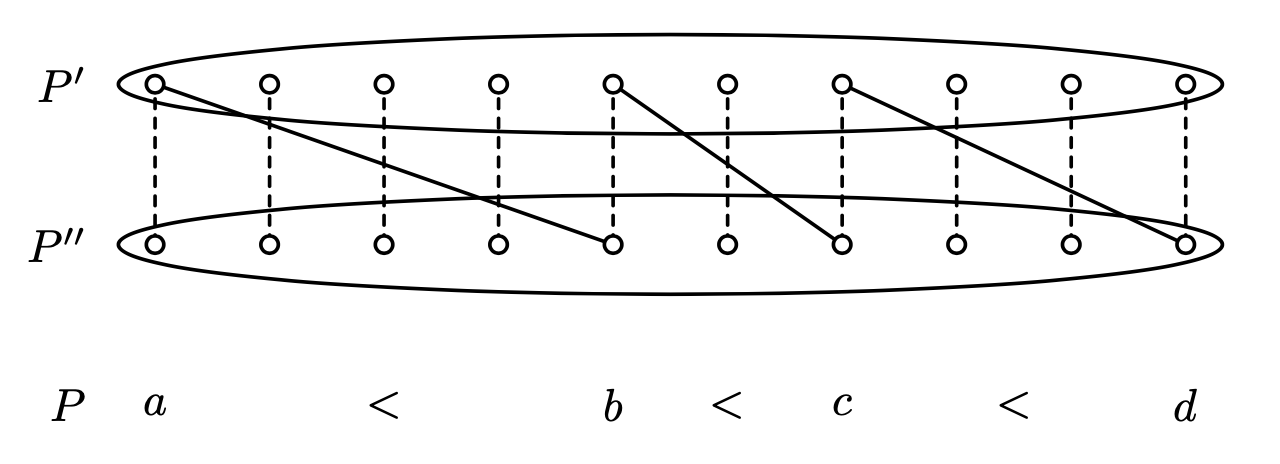
\includegraphics[width=0.7\linewidth]{Dilworth.png}$$

\subsection{Теорема про цепи/антицепи в бесконечном порядке}
\textbf{Формулировка.} В каждом бесконечном порядке есть бесконечная цепь или бесконечная антицепь\\[2mm]
\indent\textbf{Доказательство.} Построим два бесконечных множества $P$ и $A$ следующим образом. На первом шаге выберем произвольный элемент порядка $x_1$. Если он сравним с бесконечным множеством $W_1$ элементов порядка, то полагаем $x_1 \in P$. В противном случае $x_1$ несравним с бесконечным множеством $W_1$ элементов порядка, полагаем $x_1 \in A$\\[2mm]
\indentНа $(k+1)$-м шаге имеем множество $\left\{x_1, \ldots, x_k\right\}$, разбитое на множества $P$ и $A$, и бесконечное множество $W_k$. При этом выполняются следующие свойства:\\
\indent(1) каждый элемент $x_i \in P$ сравним со всеми элементами в $W_k,$\\
\indent(2) каждый элемент $x_j \in A$ несравним со всеми элементами из $W_k$,\\
\indent(3) $P$ — цепь,\\
\indent(4) $A$ антицепь\\
\indentВыберем произвольно элемент $x_{k+1} \in W_k$. Множество $W_{k+1} \subseteq W_k$ состоит либо из тех элементов, которые сравнимы с $x_{k+1}$, если таких элементов бесконечно много; либо, в противном случае, оно состоит из тех элементов, которые несравнимы с $x_{k+1}$. В первом случае помещаем $x_{k+1}$ в $P$, во втором — в $A$\\[2mm]
\indentИнвариант цикла сохраняется. Множество $W_{k+1}$ бесконечно по построению, как и свойства $(1),(2)$. Поскольку $x_{k+1} \in W_k$, то если $x_{k+1} \in P$, то $x_{k+1}$ сравнимо со всеми $x_i \in P$; а если $x_{k+1} \in A$, то $x_{k+1}$ несравнимо со всеми $x_i \in A$\\[2mm]
\indentПоскольку на каждом шаге множество $W_{k+1}$ бесконечно, описанный процесс продолжается бесконечно долго. Получаем в итоге бесконечную последовательность $\left(x_1, \ldots, x_n, \ldots\right)$, элементы которой разбиты на два множества $P$ и $A$. Правило построения гарантирует, что $P$—линейный порядок (все пары сравнимы), а $A$-антицепь (все пары несравнимы). Хотя бы одно из этих множеств бесконечно, откуда следует теорема\qed


\subsection{Контрпример к “теореме Дилуорса с мощностями”: пример бесконечного порядка, не разбивающегося на конечное число цепей и не имеющего бесконечной антицепи}
Рассмотрим $\mathbb{N}^d$ с покоординатым сравнением:
$$x=\left(x_1, \ldots, x_d\right) \leqslant\left(y_1, \ldots, y_d\right)=y \quad \Leftrightarrow \quad x_i \leqslant y_i \text { для всех }i$$
В этом порядке есть сколь угодно большие антицепи\\[2mm]
\indent\textbf{Пример.} Для любого $a \in \mathbb{N}$ множество
$$H_a=\left\{x \in \mathbb{N}^d: \sum_{i=1}^d x_i=a\right\}$$
является антицепью. Действительно, если суммы координат двух различных векторов $x, y$ равны, то одна из координат больше в векторе $x$, а какая-то другая больше в векторе $y$. При $d \geqslant 2$ и больших значениях $a$ множество $H_a$ велико: оно содержит $\binom{a+d-1}{d-1}$ векторов, что стремится к бесконечности при $a \rightarrow \infty$\\[2mm]
\indentКаждая цепь содержит не более одного элемента любой антицепи, поэтому порядок ($\mathbb{N}^d, \leqslant$) невозможно разбить на конечное количество цепей. Разбиение на счётное количество цепей тривиально, поскольку $\mathbb{N}^d$ счётно\\[2mm]
\indentОднако бесконечных антицепей в этом порядке нет\qed


\subsection{Соображения о симметрии в задачах на вероятность: примеры задач}
Возьмем в качестве вероятностного пространства множество всех слов длины $n$ в алфавите размера $k$
\subsubsection*{Задача про монотонный результат}
\indent Пусть $k=3,\ n=10$. Алфавит — множество $\{1, 2, \ldots, 10\}$. Исходы — последовательности длины 3 из различных букв алфавита\\[2mm]
\indent Определим вероятность наступления события «последовательность монотонно убывающая». Всего исходов $A^3_{10}=10\cdot9\cdot8=720$. Монотонно убывающие последовательности находятся во взаимно однозначном соответствии с 3-элементными подмножествами множества [10], поэтому их $\binom{10}{3}=\displaystyle\frac{720}{6}=120$. Тогда вероятность равна $\displaystyle\frac{120}{720}=\displaystyle\frac{1}{6}$\qed\\[2mm]
\indent Можно рассуждать и со стороны симметрии вероятностей. Любому благоприятному исходу $a b c$ соответствует 5 неблагоприятных исходов, получающихся перестановками букв $a, b$ и $c$: $acb, bac, bca,$ $cab, cba$. Таким образом, благоприятных исходов в 5 раз меньше, чем неблагоприятных, а, значит, вероятность интересующего нас события равна $\frac{1}{6}$ (и опять же, неважно, сколько исходов это событие содержит)\qed

\subsubsection*{Задача про сумму очков при подбрасывании нескольких игральных костей, которая делится на 3}
Вероятностное пространство: последовательности $\left(x_1, x_2, x_3\right)$ длины 3, состоящие из целых чисел в диапазоне от 1 до 6. Все исходы равновозможны\\[2mm]
\indentНайдём вероятность события «сумма чисел в последовательности делится на 3 ». Посчитать число всех исходов нетрудно: их $6^3=216$. Воспользуемся методом разбиения на кусочки для определния числа благоприятных исходов\\
\indentСреди 6 исходов $(x_1, x_2, 1),(x_1, x_2, 2),(x_1, x_2, 3),$ $(x_1, x_2, 4),(x_1, x_2, 5),(x_1, x_2, 6)$ ровно 2 благоприятных\\
\indentПоэтому доля благоприятных исходов будет равна $\frac{1}{3}$, это и составляет искомую вероятность\qed

\subsubsection*{Пример про вероятность вытянуть билет, который выучил, если идёшь первым или последним}
Десять учеников сдают экзамен по десяти билетам. Ученики по очереди заходят в кабинет и вытягивают случайный билет из оставшихся (в частности, последний берет единственный оставшийся билет). Вася выучил только один билет. Какова вероятность, что Васе достанется билет, который он знает, если \textbf{а)} Вася тянет билет первым? \textbf{b)} Вася тянет билет последним?\\[2mm]
\indentВ пункте (a) ясно, что Вася вытягивает случайно и равновозможно один из 10 билетов. Поэтому вероятность вытянуть благоприятный билет $\frac{1}{10}$\\[2mm]
\indent Чтобы ввести вероятностное пространство в пункте \textbf{(b)}, занумеруем студентов числами от 1 до 10 в порядке очереди. Билеты также занумеруем числами от 1 до 10, номер 10 присвоим тому билету, который Вася выучил. Тогда исходами будут перестановки чисел от 1 до 10. Все исходы равновозможны. Процесс последовательного выбора билетов как раз и представляется в виде дерева последовательного случайного выбора: сначала случайно и равновозможно выбирается билет, который берёт первый студент, затем случайно и равновозможно выбирается билет, который берёт второй студент и т.д.\\[2mm]
\indentСобытие, вероятность которого нас интересует, — на 10-м месте стоит билет номер 10 (Вася идёт последним и знает только билет №10). Всего исходов 10!, а благоприятных — 9!. Искомая вероятность равна $\frac{9 !}{10 !}=\frac{1}{10}$\qed\\[2mm]

\textbf{Не обязательно, но тоже на симметрию}\\
Примером задачи на симметрию является п.\ref{2.37}\\[2mm]
\indent\textbf{Задача про лототрон}\\
В лототроне 36 шаров, пронумерованных числами от 1 до 36 . Вытаскиваем два шара без возвращения. То есть вероятностное пространство - размещения из 36 по 2. Событие $A=$ «первый шар чётный», событие $B=$ «второй шар чётный». Независимы ли они?

Вместо размещений в качестве вероятностного пространства можно рассматривать любые упорядоченные пары чисел от 1 до 36 , но при этом нужно считать, что вероятности пар $(a, a)$ равны 0 , а вероятности всех остальных пар одинаковы, то есть распределение неравномерное. При таком выборе вероятностного пространства мы опять получаем события $A=A^{\prime} \times V, B=U \times B^{\prime}$. Но теперь эти события не являются независимыми

Вероятности событий $A$ и $B$ равны, что ясно из симметрии. Значение этих вероятностей $-1 / 2$ (на нужное место выбираем один из 18 чётных шаров, на второе место ставим какой угодно из оставшихся)

Равенство $$\textbf{Pr}[A \cap B]=\textbf{Pr}[B] \cdot \textbf{Pr}[A \mid B]=\textbf{Pr}[B] \cdot \textbf{Pr}[A]$$ не выполняется:
$$
\boldsymbol{\operatorname { P r }}[A \cap B]=\frac{18 \cdot 17}{36 \cdot 35} \neq \frac{18}{36} \cdot \frac{18}{36}=\textbf{Pr}[A] \cdot \textbf{Pr}[B],
$$

поэтому события не являются независимыми. Вероятность того, что второй шар чётный при условии, что первый шар чётный, меньше вероятности, что второй шар чётный\qed


\subsection{Задача про сумасшедшую бабку}
\textbf{Формулировка.} В самолёт по очереди заходят 100 пассажиров. Первый садится на случайное место. Каждый следующий садится на своё место, если оно свободно, и на случайное свободное место, если его место занято. Какова вероятность того, что последний пассажир сядет на своё место?

\subsubsection*{Неформальное решение}
Перед посадкой последнего пассажира может быть свободно либо его место, либо место первого пассажира. Если кто-то уже занял место первого пассажира раньше, то оставшиеся после этого пассажиры смогут сесть согласно купленным билетам, свободными останутся ровно их места. А значит, если место первого пассажира перед заходом последнего уже занято, то место последнего свободно и он на него и сядет\\[2mm]
\indentПолучается, что все исходы принадлежат ровно одному из двух событий: «последний пассажир сел на своё место» и «последний пассажир сел на место первого пассажира». Значит, в сумме вероятности этих событий дают 1\\[2mm]
\indentКроме того, вероятности этих событий одинаковы: если первый и последний пассажиры обменяются билетами, это не изменит рассадку, т.к. действия первого и последнего пассажиров не зависят от номера билета. Но события при этом переставляются: исходы, которые были в первом событии, попадают теперь во второе, и наоборот\\[2mm]
\indentИтак, вероятности двух указанных событий равны и в сумме дают 1. Поэтому каждая из них равна $1 / 2$\qed


\subsubsection*{Формальное решение}
Определим возможные исходы. Занумеруем пассажиров в порядке очереди числами от 1 до 100. Исходом будет рассадка пассажиров по местам, т.е. некоторая перестановка чисел от 1 до 100. Вероятности исходов неодинаковы. Их можно определить процессом последовательного случайного выбора: первый пассажир выбирает позицию в перестановке согласно  равномерному распределению; $i$-й по очереди пассажир выбирает либо своё место, если оно свободно, с вероятностью 1 (вероятности остальных вариантов при этом равны 0), в противном случае он выбирает одно из свободных мест согласно равномерному распределению на них\\[2mm]
\indentТаким образом, мы получаем представление нашего вероятностного пространства в виде дерева. Чтобы определить вероятность исхода, нужно перемножить вероятности для всех выборов на пути из корня в соответствующий лист. Полученное распределение не равномерное. Например, любая перестановка, в которой первый пассажир сидит на своём месте, а какой-то пассажир — не на своём, имеет вероятность 0\\[2mm]
\indentЗаметим, что вероятности перестановок-исходов зависят от раздачи билетов, т.е. соответствия между пассажирами и местами. Обозначим через $\pi$ это соответствие: у первого пассажира билет на место $\pi(1)$, у второго — на место $\pi(2)$ и т.д. Мы фактически определили не одно распределение, а 100! распределений на одном и том же вероятностном пространстве. Одно такое распределение получается из другого перенумерацией мест, т.е. перестановкой исходов\\[2mm]
\indentОбозначим через $G_\pi$ событие «последний пассажир сел на своё место», а через $B_\pi$ — его дополнение, т.е. «последний пассажир сел на место первого». Каждый исход попадает в одно из этих событий, поэтому
$$\mathbf{P r}_\pi\left[G_\pi\right]+\mathbf{P r}_\pi\left[B_\pi\right]=1$$
\indentИндекс $\pi$ указывает на распределение, задаваемое раздачей билетов $\pi$\\[2mm]
\indent Вероятности интересующих нас событий не зависят от раздачи билетов, то есть $\textbf{Pr}_\pi\left[G_\pi\right]=\textbf{Pr}_\sigma\left[G_\sigma\right]$ для любых $\pi, \sigma$: при перенумерации мест перестановки, в которых последний сидит на своём месте, переходят в точности в перестановки, в которых последний сидит на своём месте\\[2mm]
\indentРассмотрим две раздачи билетов
$$
\pi=(1,2, \ldots, 99,100), \sigma=(100,2, \ldots, 99,1)
$$
(первый и последний обменялись билетами)\\[2mm]
\indentДля любой рассадки $\alpha$ выполняется равенство
$$
\mathbf{P r}_\pi[\alpha]=\mathbf{P r}_\sigma[\alpha] .
$$

\indentДействительно, при вычислении вероятности исхода $\alpha$ все числа на пути из корня дерева случайного выбора в лист $\alpha$ одинаковы в обоих случаях. Первое равно 1/100 (т.к. первый пассажир выбирает одно из 100 мест согласно равномерному распределению). Последнее равно 1 (т.к. у последнего нет выбора). Все промежуточные вероятности выборов равны, так как $\pi$ и $\sigma$ различаются только местами первого и последнего и это различие не меняет количества возможных выборов для $i$-го пассажира\\[2mm]
\indentОднако интересующие нас события переставляются: $\alpha \in G_\pi$ (то есть $a_{100}=100$) тогда и только тогда, когда $\alpha \in B_\sigma$ (последний пассажир садится либо на своё место, либо на место первого). Поэтому
$$
\mathbf{P r}_\pi\left[G_\pi\right]=\mathbf{P r}_\sigma\left[B_\sigma\right]
$$\\[2mm]
\indentПоскольку $\mathbf{Pr}_\sigma\left[G_\sigma\right]=\mathbf{P r}_\pi\left[G_\pi\right]$, то получаем $\mathbf{P r}_\sigma\left[G_\sigma\right]=\mathbf{P r}_\sigma\left[B_\sigma\right]$, то есть $\mathbf{P r}_\sigma\left[G_\sigma\right]=1 / 2$\qed


\subsection{Лемма про попарно несовместные события. Оценка объединения. Формула включений и исключений для вероятностей}
\subsubsection*{Лемма}
\textbf{Формулировка.} Если события $A_i$ попарно несовемстны, то $$\textbf{Pr}\left[\bigcup_{i=1}^n A_i\right]=\sum_{i=1}^n \textbf{Pr}[A_i]$$
\indent\textbf{Доказательство.} Сумма вероятностей по объединению семейства попарно несовместных событий после перегруппировки слагаемых превращается в сумму по событиям вероятностей события:
$$
\textbf{Pr}\left[\bigcup_{i=1}^n A_i\right]=\sum_{x \in \bigcup_{i=1}^n A_i} \textbf{Pr}[x]=\sum_{i=1}^n \sum_{x \in A_i} \textbf{Pr}[x]=\sum_{i=1}^n \textbf{Pr}\left[A_i\right]
$$
\indentПри переходе от второй суммы к третьей возможно, что некоторые исходы попадут в несколько слагаемых с разными значениями $i$. Однако события несовместны, поэтому вероятности таких исходов равны 0, так что равенство выполняется\qed

\subsubsection*{Оценка объединения}
\textbf{Формулировка.} Для любых событий $A_1,\ldots, A_n\subseteq U$ выполняется $$\textbf{Pr}\left[\bigcup_{i=1}^n A_i\right]\leqslant\sum_{i=1}^n \textbf{Pr}[A_i]$$
\indent\textbf{Доказательство.} И в левой, и в правой части стоит сумма вероятностей исходов\\
\indentКаждый исход в левой сумме встречается и в правой (возможно, не один раз). Неравенство выполняется, так как вероятности неотрицательные\qed

\subsubsection*{Формула включений и исключений для вероятностей}
\textbf{Формулировка.} Для всякой вероятностной модели и для произвольных множеств $A_1, \ldots, A_n \subseteq U$ верно $$
\begin{aligned}
\textbf{Pr}\left[A_1 \cup A_2 \cup \cdots \cup A_n\right] & =\sum_i \textbf{Pr}\left[A_i\right]-\sum_{i<j} \textbf{Pr}\left[A_i \cap A_j\right]+\cdots= \\
& =\sum_{\varnothing \neq S \subset\{1,2, \ldots, n\}}(-1)^{|S|+1} \textbf{Pr}\left[\bigcap_{i \in S} A_i\right]
\end{aligned}$$
\indent\textbf{Доказательство.} Снова используем индикаторные функции. Мы использовали такое равенство $$
\chi_A(x)=1-\left(1-\chi_{A_1}(x)\right)\left(1-\chi_{A_2}(x)\right) \ldots\left(1-\chi_{A_n}(x)\right),
$$
которое переписывается как
$$\chi_A(x)=\sum_{S \neq \varnothing}(-1)^{|S|+1} \chi_{A_S}(x), \quad \text { где } A_S=\bigcap_{i \in S} A_i .$$
Вероятность $A$ выражается как сумма по всему вероятностному пространству
$$\textbf{Pr}[A]=\sum_{u \in U} \textbf{Pr}[u] \chi_A(u)$$
(каждый благоприятный исход даёт вклад 1 в сумму, неблагоприятные исходы дают вклад 0$)$.
Для $A=A_1 \cup A_2 \cup \cdots \cup A_n$ подставим в эту сумму наше равенство и получим
$$
\begin{aligned}
\textbf{Pr}[A] & =\sum_{x \in U} \textbf{Pr}[x] \chi_A(x)=\sum_{x \in U} \textbf{Pr}[x] \sum_{S \neq \varnothing}(-1)^{|S|+1} \chi_{A_S}(x)= \\
& =\sum_{S \neq \varnothing}(-1)^{|S|+1} \sum_{x \in U} \textbf{Pr}[x] \chi_{A_S}(x)=\sum_{S \neq \varnothing}(-1)^{|S|+1} \textbf{Pr}\left[A_S\right]
\end{aligned}
$$
это и есть формула включений и исключений\qed
\label{2.34}


\subsection{Симметричность определения независимости событий. Формула полной вероятности. Формула Байеса}
\subsubsection*{Симметричность определения независимости событий}
\textbf{Формулировка.} \textbf{Независимые события} $A$ и $B$, если $\boxed{\textbf{Pr}[A]=\textbf{Pr}[A|B]}$\\[2mm]
\indentЭквивалентное определение независимости событий:
$\boxed{\textbf{Pr}[A \cap B]=\textbf{Pr}[B] \cdot \textbf{Pr}[A|B]=\textbf{Pr}[B] \cdot \textbf{Pr}[A]}$\\[2mm]
\indent Остюда ясно, что отношение независимости событий \textit{симметрично}, если вероятности событий положительные. Это определение применимо и к событиям нулевой вероятности

\subsubsection*{Формула полной вероятности}
\textbf{Формулировка.} Пусть $B_1, \ldots, B_n$ - разбиение вероятностного пространства $U$, то есть $U=B_1 \cup \ldots \cup B_n$, где $B_i \cap B_j=\varnothing$ при $i \neq j$. Пусть также $\textbf{Pr}\left[B_i\right]>0$ для всякого $i$. Тогда для всякого события $A$
$$\boxed{
\textbf{Pr}[A]=\sum_{i=1}^n \textbf{Pr}\left[A | B_i\right] \cdot \textbf{Pr}\left[B_i\right]}
$$
\indent\textbf{Доказательство.} Прямое вычисление:
$$
\textbf{Pr}[A]=\sum_{i=1}^n \textbf{Pr}\left[A \cap B_i\right]=\sum_{i=1}^n \textbf{Pr}\left[A | B_i\right] \cdot \textbf{Pr}\left[B_i\right]
$$
где первое равенство получается по формуле сложения вероятностей несовместных событий (лемма из \ref{2.34}), а второе равенство — по определению условной вероятности\qed

\subsubsection*{Формула Байеса}
\textbf{Формулировка.} Если вероятности событий $A$ и $B$ положительны, то $$\boxed{\textbf{Pr}[A|B]=\textbf{Pr}[A]\cdot\displaystyle\frac{\textbf{Pr}[B|A]}{\textbf{Pr}[B]}}$$
\indent\textbf{Доказательство.} Выразим вероятность события $A \cap B$ через условные вероятности двумя способами:
$$
\textbf{Pr}[A \cap B]=\textbf{Pr}[B] \cdot \textbf{Pr}[A | B]=\textbf{Pr}[A] \cdot \textbf{Pr}[B | A] .
$$
Формула Байеса получается из второго равенства делением обеих его частей на $\textbf{Pr}[B]$\qed

\subsection{Парадокс Симпсона}
\textbf{Формулировка.} Существует такое вероятностное пространство и события $A,B,C,D,E$, что $\textbf{Pr}[A|B]<\textbf{Pr}[A|D];\ \textbf{Pr}[A|C]<\textbf{Pr}[A|E];\ \textbf{Pr}[A|B\cup C]>\textbf{Pr}[A|D\cup E]$\\[2mm]
\indent\textbf{Доказательство.} Будем искать пример в предположении, что события $B, C, D, E$ не пересекаются. Формула полной вероятности справедлива и для условных вероятностей: ограничим вероятностное распределение на событие-условие. Поэтому
$$
\begin{aligned}
& \textbf{Pr}[A | B \cup C]=\textbf{Pr}[B | B \cup C] \cdot \textbf{Pr}[A | B]+\textbf{Pr}[C | B \cup C] \cdot \textbf{Pr}[A | C], \\
& \textbf{Pr}[A | D \cup E]=\textbf{Pr}[D | D \cup E] \cdot \textbf{Pr}[A | D]+\textbf{Pr}[E | D \cup E] \cdot \textbf{Pr}[A | E] .
\end{aligned}
$$

Мы воспользовались такими равенствами
$$
\begin{array}{ll}
\textbf{Pr}[A | B]=\textbf{Pr}[A | B \cap(B \cup C)], & \textbf{Pr}[A | C]=\textbf{Pr}[A | C \cap(B \cup C)], \\
\textbf{Pr}[A | D]=\textbf{Pr}[A | D \cap(D \cup E)], & \textbf{Pr}[A | E]=\textbf{Pr}[A | E \cap(D \cup E)] .
\end{array}
$$
(события-условия в левых и правых частях этих равенств одинаковы)\\
\indentОбозначим для краткости
$$
p_1 =\textbf{Pr}[A | B],\ p_2 =\textbf{Pr}[A | D],\ p_3=\textbf{Pr}[A | C],\ p_4=\textbf{Pr}[A | E];
\alpha =\textbf{Pr}[B | B \cup C],\ \beta =\textbf{Pr}[D | D \cup E]
$$
В таких обозначениях нужно удовлетворить неравенствам
$$
p_1<p_2, \quad p_3<p_4, \quad \alpha p_1+(1-\alpha) p_3>\beta p_2+(1-\beta) p_4
$$
(заметим, что $\textbf{Pr}[B | B \cup C]+\textbf{Pr}[C | B \cup C]=1$ и $\textbf{Pr}[D | D \cup E]+\textbf{Pr}[E | D \cup E]=1$)\\
\indentМножество
$$
\{x: x=\lambda p+(1-\lambda) q, 0 \leqslant \lambda \leqslant 1\}
$$
является отрезком $[p ; q]$. Поэтому неравенства выполняются при подходящих $\alpha, \beta$, если
$$
p_3<p_4<p_1<p_2
$$
(отрезки $\left[p_3 ; p_1\right]$ и $\left[p_4 ; p_2\right]$ в таком случае пересекаются по внутренней точке)\qed


\subsection{Вычисление вероятности события “два случайных
\texorpdfstring{$k$}{k}-элементных подмножества
\texorpdfstring{$n$}{n}-элементного множества не пересекаются”. Асимптотика при \texorpdfstring{$k\approx\sqrt{n}$}{k=vn}}
\label{2.37}
Из $n$-элементного множества выбираются случайно, равновозможно и независимо два $k$-элементных множества $X$ и $Y$. Какова вероятность события «$X \cap Y=\varnothing$»?\\
\indentУсловие означает, что вероятностное пространство — пары $(X, Y)$ $k$-элементных подмножеств $n$-элементного множества, вероятности всех исходов одинаковы\\
\indentДля любых подмножеств $A$ и $B$ данного $n$-элементного множества количество исходов в событиях «$Y=A$» и «$Y=B$» одинаково, как и количество тех $X$, которые не пересекаются с $Y$. Поэтому вероятности условных событий «$X \cap Y=\varnothing | Y=A$» и «$X \cap Y=\varnothing | Y=B$» одинаковы\\
\indentИз формулы полной вероятности получаем для любого множества $A,|A|=k$ :
$$
\begin{aligned}
& \textbf{Pr}[X \cap Y=\varnothing]=\sum_{|S|=k} \textbf{Pr}[X \cap Y=\varnothing \mid Y=S] \textbf{Pr}[Y=S]= \\
& =\textbf{Pr}[X \cap Y=\varnothing \mid Y=A] \cdot \sum_{|S|=k} \textbf{Pr}[Y=S]=\textbf{Pr}[X \cap Y=\varnothing \mid Y=A]
\end{aligned}
$$
\indentПусть $A=\{1, \ldots, k\}$. Вероятность выбрать $k$-элементное множество $X$, которое не содержит ни одного элемента из $A$, равна
$$\displaystyle\frac{\binom{n-k}{k}}{\binom{n}{k}}$$
(в числителе стоит количество $k$-элементных подмножеств в дополнении к $A$, а в знаменателе — количество $k$-элементных подмножеств в $n$-элементном множестве)\\
\indentПреобразуем это выражение:
$$
\displaystyle\frac{\binom{n-k}{k}}{\binom{n}{k}}=\left(1-\frac{k}{n}\right) \cdot\left(1-\frac{k}{n-1}\right) \cdot \ldots \cdot\left(1-\frac{k}{n-k+1}\right) \leqslant\left(1-\frac{k}{n}\right)^k
$$
\indentПри больших $n$ и $k \approx c \sqrt{n}$ последнее выражение оценивается как $e^{-c^2}$. Получаем, что весьма малые случайные подмножества большого конечного множества почти заведомо пересекаются\qed


\subsection{Линейность математического ожидания. Вычисление математического ожидания случайной величины “размер пересечения двух случайных \texorpdfstring{$k$}{k}-элементных подмножеств \texorpdfstring{$n$}{n}-элементного множества”}
\subsubsection*{Линейность математического ожидания}
\textbf{Формулировка.} Пусть $f: U \rightarrow \mathbb{R}$ и $g: U \rightarrow \mathbb{R}$ — две случайные величины на одном и том же вероятностном пространстве с одним и тем же вероятностным распределением. Тогда $$\mathbf{E}[f+g]=\mathbf{E}[f]+\mathbf{E}[g]$$
\textbf{\indent Доказательство.} Запишем определение и перегруппируем слагаемые:
$$\mathbf{E}[f+g]=\sum_{x \in U}(f+g)(x) \textbf{Pr}[x]=\sum_{x \in U} f(x) \textbf{Pr}[x]+\sum_{x \in U} g(x) \textbf{Pr}[x]=\mathbf{E}[f]+\mathbf{E}[g]$$\qed

\subsubsection*{Пример вычисления мат.ожидания случайной величины}
Пусть вероятностное пространство — пары $k$-элементных подмножеств $n$-элементного множества, распределение равномерное. Случайная величина $S=|X \cap Y|$ равна размеру пересечения этих подмножеств. Определим чему равно математическое ожидание $S$\\[2mm]
\indentКоличество элементов в подмножестве равно сумме значений индикаторной функции этого множества по всем элементам множества. Поэтому случайная величина $S$ разлагается в сумму случайных величин
$$
s_{1}+s_{2}+\ldots+s_{n}, \quad \text { где } s_{j}(X, Y)=\left\{\begin{array}{l}
1, \text { если } j \in X \cap Y \\
0, \text { иначе. }
\end{array}\right.
$$
Математическое ожидание случайной величины $s_{j}$ выражается как

$$
\mathbf{E}\left[s_{j}\right]=1 \times \textbf{Pr}\left[A_{j}\right]+0 \times \textbf{Pr}\left[\bar{A}_{j}\right]=\textbf{Pr}\left[A_{j}\right]
$$
где $A_{j}$ — событие «$j \in X \cap Y$»\\
\indentСобытия «$j\in X$» и «$j \in Y$» независимы. Поэтому
$$
\textbf{Pr}\left[A_{j}\right]=\textbf{Pr}[j \in X] \cdot \textbf{Pr}[j \in Y]=\displaystyle\frac{\binom{n-1}{k-1}}{\binom{n}{k}}\cdot\displaystyle\frac{\binom{n-1}{k-1}}{\binom{n}{k}}=\frac{k^{2}}{n^{2}}$$
\indentОкончательно получаем
$$
\mathbf{E}[S]=\mathbf{E}\left[s_{1}+s_{2}+\ldots+s_{n}\right]=\sum_{j=1}^{n} \mathbf{E}\left[s_{j}\right]=n \cdot \frac{k^{2}}{n^{2}}=\frac{k^{2}}{n}
$$
\indentТаким образом, при $k \approx c \sqrt{n}$ имеем $\mathbf{E}[S] \approx c^{2}$\qed
\label{2.38}

\subsection{Линейность математического ожидания. Парадокс дней рождения}
Линейность математического ожидания доказана в \ref{2.38}
\subsubsection*{Парадокс дней рождения}
Рассмотрим $n$ случайных людей и посмотрим на количество совпадений дней рождения у них, то есть на количество пар людей, имеющих день рождения в один день. Определим среднее значение этого числа\\[2mm]
\indentУточним вопрос и упростим его. Предполагаем, что дни рождения у разных людей независимы, а в году 365 дней. То есть, вероятностное пространство: всюду определённые функции из $n$-элементного множества людей $\left\{x_{1}, \ldots, x_{n}\right\}$ в 365 элементное множество дней в году. Все исходы равновозможные\\[2mm]
\indentОбозначим случайную величину, равную количеству пар людей с совпадающими днями рождения, через $F$. Нам требуется посчитать математическое ожидание случайной величины $F$\\[2mm]
\indentОбозначим через $g_{i j}$ случайную величину, равную 1, если у людей $x_{i}$ и $x_{j}$ дни рождения совпадают, и равную 0 в противном случае. Тогда
$$
F=\sum_{i<j} g_{i j}
$$
\indentПодсчитаем математическое ожидание случайной величины $g_{i j}$. Вероятность того, что у двух случайных людей дни рождения совпадают, равна $1 / 365$, так что с вероятностью $1 / 365$ случайная величина равна 1, и с вероятностью 
$(1-1 / 365)$ равна 0. Поэтому $\mathbf{E}\left[g_{i j}\right]=1 / 365$ (для всякой пары $i, j$). Для математического ожидания $F$ из линейности получаем
$$
\mathbf{E}[F]=\mathbf{E}\left[\sum_{i<j} g_{i j}\right]=\sum_{i<j} \mathbf{E}\left[g_{i j}\right]=\sum_{i<j} \frac{1}{365}=\frac{n(n-1)}{2 \cdot 365}
$$
\indentЕсли число людей $n$ больше 27, то $\mathbf{E}[F]>1$, то есть стоит ожидать\footnote{Если посчитать точно, то при $n=28$ вероятность того, что будет не меньше одного совпадения дней рождения, равна $\approx 0.65 ;$ математическое ожидание числа совпадений $\approx 1.03$}, что будет не меньше одного совпадения дней рождений\qed

\subsection{Оценка среднего. Теорема о существовании в графе большого разреза}
\subsubsection*{Оценка среднего}
\textbf{Формулировка.} Пусть $\textbf{E}[f]=C$ для какой-то случайной величины $f:U\to\mathbb{R}$. Тогда существует такой исход $u\in U$, что $f(u)\geqslant C$. Аналогично, существует и такой исход $u\in U$, что $f(u)\leqslant C$\\[2mm]
\indent\textbf{Доказательство.} Докажем от противного первое утверждение леммы, второе доказывается аналогично. Предположим, что утверждение неверно, а значит для всякого $u \in U$ верно $f(u)<C$\\
\indentТогда
$$
\mathbf{E}[f]=\sum_{u \in U} \textbf{Pr}[u] f(u)<\sum_{u \in U} \textbf{Pr}[u] C=C,
$$
противоречие\qed

\subsubsection*{Теорема о существовании в графе большого разреза}
\textbf{Формулировка.} Всякий граф $G=(V,E)$ имеет разрез размера не меньше $|E|/2$\\[2mm]
\indent\textbf{Доказательство.} Рассмотрим случайный разрез графа $G$. Мы берём равномерное распределение на множестве всех разрезов. Разрез задаётся подмножеством $S \subseteq V$: такому подмножеству ставится в соответствие разрез $(S, V \setminus S)$. Всего подмножеств (=разрезов) $2^{n}$, так что вероятность каждого разреза есть $1 / 2^{n}$. Для каждой пары вершин $x \neq y$ все четыре события \guillemetleft$x \in S, y \in S$», \guillemetleft$x \notin S, y \in S$, \guillemetleft$x \in S, y \notin S$», \guillemetleft$x \notin S, y \notin S$» имеют вероятность $1 / 4$\footnote{Сопоставьте случайным множествам двоичные строки длины $|V|$, тогда интересующие нас события состоят в том, что на позициях $x, y$ записаны конкретные значения}\\[2mm]
\indentРассмотрим случайный разрез и случайную величину $f$, равную размеру разреза и посчитаем её математическое ожидание. Для этого разобьем случайную величину в сумму более простых случайных величин. Для всякого $e \in E$ рассмотрим случайную величину $f_{e}$, равную 1, если ребро $e$ входит в разрез, и равную 0 в противном случае. Тогда $f=\displaystyle\sum_{e \in E} f_{e}$, а значит
$$
\mathbf{E}[f]=\sum_{e \in E} \mathbf{E}\left[f_{e}\right]
$$
\indent Теперь найдем для случайной величины $f_{e}$ математическое ожидание. Для всякого фиксированного ребра $e$ вероятность, что оно попадёт в разрез равна $1 / 2$. А значит, $\mathbf{E}\left[f_{e}\right]=1 / 2$ для всякого $e \in E$, откуда
$$
\mathbf{E}[f]=\sum_{e \in E} 1 / 2=|E| / 2
$$
\indentИз этого следует, что есть конкретный разрез, содержащий не меньше $|E| / 2$ рёбер\qed


\subsection{Неравенство Маркова. Примеры применения}
\textbf{Формулировка.} $\textbf{Pr}[f\geqslant\alpha]\leqslant\displaystyle\frac{\textbf{E}[f]}{\alpha}$\\[4mm]
\indent\textbf{Доказательство.} Докажем равносильное $$\textbf{E}[f]\geqslant\alpha\cdot\textbf{Pr}[f\geqslant\alpha]$$\\
$$\textbf{E}[f]=\displaystyle\sum_{x\in U}f(x)\textbf{Pr}[x]=\displaystyle\sum_{x:f(x)\geqslant\alpha}f(x)\textbf{Pr}[x] +\displaystyle\sum_{x:f(x)<\alpha}f(x)\textbf{Pr}[x]$$
Заменим в первом слагаемом $f(x)$ на $\alpha$, от этого сумма может лишь уменьшится. Во втором слагаемом заменим $f(x)$ на 0, от этого сумма также может лишь уменьшится. Получаем
$$\textbf{E}[f]\geqslant\alpha\cdot\displaystyle\sum_{x:f(x)\geqslant\alpha}\textbf{Pr}[x]+0\cdot\displaystyle\sum_{x:f(x)<\alpha}\textbf{Pr}[x]=\alpha\cdot\textbf{Pr}[f(x)\geqslant\alpha]$$\qed

\subsubsection*{Пример—1}
В лотерее на выигрыши уходит 40\% от стоимости проданных билетов. Каждый билет стоит 100 рублей. Докажите, что вероятность выиграть хотя бы 5000 рублей меньше 1\%\\
Обозначим через $X$ случайную величину, равную выигранной сумме. Тогда из условий задачи получаем, что $\textbf{E}[X] = 0, 4 \cdot 100 = 40$. Из неравенства Маркова имеем
$$\textbf{Pr}[X\geqslant5000]\leqslant\displaystyle\frac{\textbf{E}[X]}{5000}=\displaystyle\frac{40}{5000}=0,008<0,01$$\qed

\subsubsection*{Пример—2}
Пусть есть такой алгоритм $A$, работающий за среднее время $O\left(n^2\right)$, где $n$ — размер входных данных. Для наших практических целей хотелось бы, чтобы алгоритм всегда заканчивал свою работу за время $O\left(n^2\right)$. И пусть в $0,01 \%$ случаев алгоритм будет выдавать неправильный ответ

Обозначим среднее время работы алгоритма $A$ через $T$, и рассмотрим такой алгоритм: запускаем алгоритм $A$ и ждём пока он сделает $10000 \cdot T$ шагов. Если алгоритм успел выдать ответ, прекрасно. Если нет, выдаём произвольный ответ. Идея в том, что алгоритм $A$ с очень большой вероятностью закончит свою работу за $10000 \cdot T$ шагов. Действительно, обозначим через $f$ (неотрицательную) случайную величину, равную времени работы алгоритма $A$. Тогда $\textbf{E}[f]=T$. По неравенству Маркова получаем
$$
\textbf{Pr}[f>10000 \cdot T] \leqslant \frac{T}{10000 \cdot T}=1 / 10000
$$\qed\\[2mm]
Время работы нового алгоритма — $O(n^2)$, а ошибка может произойти только если старый алгоритм работал дольше $10000\cdot T$ шагов. По нашей оценке это происходит с вероятностью не больше 0.01\%


\subsection{Лемма о выражении дисперсии. Неравенство Чебышёва}
\subsubsection*{Лемма}
\textbf{Формулировка.} $\textbf{D}[f]=\textbf{E}[f^2]-\textbf{E}[f]^2$\\[4mm]
\indent\textbf{Доказательство.} Пусть $C \in \mathbb{R}$, тогда $\mathbf{E}[C \cdot f]=C \cdot \mathbf{E}[f]$. По определению математического ожидания получаем:
$$
\mathbf{E}[C \cdot f]=\sum_{x \in U} C \cdot f(x)=C \cdot \sum_{x \in U} f(x)=C \cdot \mathbf{E}[f] .
$$

Теперь распишем по определению $\mathbf{D}[f]$, воспользовавшись при этом линейностью математического ожидания (п. \ref{2.38}):
$$
\begin{aligned}
& \mathbf{D}[f]=\mathbf{E}\left[(f-\mathbf{E}[f])^2\right]=\mathbf{E}\left[f^2-2 \mathbf{E}[f] \cdot f+\mathbf{E}[f]^2\right]=\mathbf{E}\left[f^2\right]-\mathbf{E}[2 \mathbf{E}[f] \cdot f]+\mathbf{E}\left[\mathbf{E}[f]^2\right]= \\
& =\mathbf{E}\left[f^2\right]-2 \mathbf{E}[f] \cdot \mathbf{E}[f]+\mathbf{E}[f]^2=\mathbf{E}\left[f^2\right]-\mathbf{E}[f]^2
\end{aligned}
$$\qed

\subsubsection*{Неравенство Чебышёва}
\textbf{Формулировка.} $\textbf{Pr}\left[\left|f-\textbf{E}[f]\right|\geqslant\alpha\right]\leqslant\displaystyle\frac{\textbf{D}[f]}{\alpha^2}$\\[4mm]
\indent\textbf{Доказательство.} Событие $\left|f-\textbf{E}[f]\right|\geqslant\alpha$ совпадает с событием $\left|f-\textbf{E}[f]\right|^2\geqslant\alpha$. Применение неравенства Маркова к этому второму событию и даёт неравенство Чебышёва\qed

\subsection{Типичный пример независимых случайных величин. Лемма о математическом ожидании произведения независимых случайных величин}
\subsubsection*{Пример}\label{2.43}
Пусть множество исходов $U=A \times B$. Представим исходы как матричные элементы матрицы, строки которой индексированы множеством $A$, а столбцы-множеством $B$

Вероятность исхода $(a, b)$ равна $p_a q_b$, где $p$ — вероятностное распределение на $A$, а $q$ — вероятностное распределение на $B$. Пусть величина $f(a, b)$ зависит только от строки $a$, а величина $g(a, b)$ — только от столбца $b$. Тогда эти величины независимы

Действительно, пусть $f^{-1}(x)=A_1 \times B, g^{-1}(y)=A \times B_1$. Тогда
$$
\begin{aligned}
& \textbf{Pr}[f=x]=\textbf{Pr}\left[A_1\right], \quad \textbf{Pr}[g=y]=\textbf{Pr}\left[B_1\right] \\
& \textbf{Pr}[f=x \wedge g=y]=\sum_{a \in A_1} \sum_{b \in B_1} p_a q_b=\textbf{Pr}\left[A_1\right] \cdot \textbf{Pr}\left[B_1\right]
\end{aligned}
$$

\subsubsection*{Лемма}
\textbf{Формулировка.} Если $f, g$ независимы, то $\textbf{E}[f\cdot g] = \textbf{E}[f]\cdot \textbf{E}[g]$\\[4mm]
\indent\textbf{Доказательство.} Математическое ожидание случайной величины $f: U \rightarrow \mathbb{R}$ записывается в виде
$$
\mathbf{E}[f]=\sum_{x \in f(U)} x \cdot \textbf{Pr}[f=x]
$$
(сгруппируем слагаемые с одинаковым значением $f$ в определении математического ожидания). Поэтому
$$
\begin{aligned}
& \mathbf{E}[f] \cdot \mathbf{E}[g]=\left(\sum_{x \in f[U]} x \cdot \textbf{Pr}[f=x]\right) \cdot\left(\sum_{y \in g[U]} y \cdot \textbf{Pr}[g=y]\right)= \\
& =\sum_{x \in f[U]} \sum_{y \in g[U]} x y \cdot \textbf{Pr}[f=x] \mathbf{P r}[g=y]=\sum_{x \in f[U]} \sum_{y \in g[U]} x y \cdot \textbf{Pr}[f=x \wedge g=y]= \\
& =\sum_{z \in f g[U]} z \textbf{Pr}[f g=z]=\mathbf{E}[f g]
\end{aligned}
$$

Второе равенство — это раскрытие скобок, третье — применение определения независимых случайных величин, последнее получается группировкой одинаковых слагаемых\qed

\subsection{Неравенство Хёфдинга–Чернова}
\textbf{Формулировка.} Пусть $\varepsilon>0$, тогда
$$\pr{\left|X_n-\frac{n}{2}\right|>\varepsilon n}=\pr{\left|\xi_n-\frac{1}{2}>\varepsilon\right|}<2e^{-2\varepsilon^2n}$$\\[4mm]
\indent\textbf{Доказательство.} Это неравенство получается как частный случай неравенства Маркова для подходящим образом подобранной функции от величины $X_{n}$.

Введём случайные величины $Y_{n}=2 X_{n}-n$. Если $X_{n}$ равна сумме $n$ случайных величин, принимающих независимо и равновероятно значения 0 и 1, то $Y_{n}$ равна сумме $n$ величин $y_{i}$, каждая из которых независимо принимает случайно и равновероятно значения —1 и +1

Теперь возьмём экспоненту от $Y_{n}$ с удачным основанием (которое выберем позже). Определим случайную величину

$$
Z_{n}=e^{\lambda Y_{n}}=\prod_{i} e^{\lambda y_{i}}=\prod_{i} z_{i}
$$

Величины $z_{i}$ независимы (это частный случай примера из \ref{2.43}). Поэтому мат. ожидание произведения равно произведению мат. ожиданий сомножителей:

$$
\mathbf{E}\left[Z_{n}\right]=\prod_{i} \mathbf{E}\left[e^{\lambda y_{i}}\right]=\left(\frac{e^{\lambda}+e^{-\lambda}}{2}\right)^{n}=(\operatorname{ch} \lambda)^{n}
$$

Интересующее нас событие $X_{n}-n / 2>\varepsilon n$ записывается через случайную величину $Y_{n}$ как $Y_{n}>2 \varepsilon n$, а через величину $Z_{n}$ как $Z_{n}>e^{2 \lambda \varepsilon n}$

Применим неравенство Маркова к случайной величине $Z_{n}$:

$$
\textbf{Pr}\left[Z_{n}>e^{2 \lambda \varepsilon n}\right] \leqslant \frac{\mathbf{E}\left[Z_{n}\right]}{e^{2 \lambda \varepsilon n}}=\left(\frac{\operatorname{ch} \lambda}{e^{2 \lambda \varepsilon}}\right)^{n}
$$

Осталось выбрать $\lambda$, чтобы сделать дробь в основании степени поменьше. Для этого нужно неравенство
$$
\operatorname{ch} x \leqslant e^{x^{2} / 2}
$$

Подставляя это неравенство, получаем при $\lambda=2 \varepsilon$

$$
\textbf{Pr}\left[Z_{n}>e^{2 \lambda \varepsilon n}\right] \leqslant e^{\left(2 \varepsilon^{2}-4 \varepsilon^{2}\right) n}
$$\qed\\[4mm]
\indent\textbf{Доказательство $\operatorname{ch} x \leqslant e^{x^{2} / 2}$.} Разложим экспоненту в ряд Тейлора:

$$
e^{x}=\sum_{k=0}^{\infty} \frac{x^{k}}{k !}
$$

Ряд для гиперболического косинуса получается отсюда почленным сложением рядов. Остаются только слагаемые в чётных степенях:

$$
\operatorname{ch} x=\sum_{k=0}^{\infty} \frac{x^{2 k}}{(2 k) !}
$$
\indentВторой ряд получается подстановкой $x^{2} / 2$ в ряд для экспоненты. Опять есть только слагаемые для чётных степеней:

$$
e^{x^{2} / 2}=\sum_{k=0}^{\infty} \frac{x^{2 k}}{2^{k} k !}
$$

Осталось заметить, что при каждом $k$ выполняется

$$
\frac{1}{(2 k) !} \leqslant \frac{1}{2^{k} k !}
$$

нужная формула получается почленным сравнением рядов\qed

\subsection{Существование и единственность деления с остатком. Утверждение о корректности суммы, разности и произведения вычетов}
\subsubsection*{Существование и единственность деления с остатком}\label{2.45}
\textbf{Формулировка.} Деление с остатком всегда возможно, причем единственным образом\\[4mm]
\indent\textbf{Доказательство.} \textit{Единственность}. Если $a=b q+r=b q^{\prime}+r^{\prime}$, то $r-r^{\prime}=b\left(q^{\prime}-q\right)$ и потому $r-r^{\prime}$ делится на $b$. Но оба числа $r, r^{\prime}$ находятся в интервале $0,1, \ldots, b-1$, так что их разность (если из большего вычесть меньшее) не больше $b-1$ и делится на $b$. Поэтому $r=r^{\prime}$, откуда и $q=q^{\prime}$\\[2mm]
\indent \textit{Существование} для неотрицательных чисел докажем индукцией по $a$. Для $a=0$ частное и остаток равны нулю: $0=0 \cdot b+0$. Если $a=b q+r$, то $a+1=b q+(r+1)$. При этом $r+1 \leqslant b$, так как $r<b$. Если $r+1<b$, то для $a+1$ получаем частное $q$ и остаток $r+1$. Если же $r+1=b$, то $a+1=b q+b=b(q+1)+0$, получаем частное $q+1$ и остаток 0

Для отрицательных чисел: разделим $-a$ на $b$ с остатком, получим $-a=b q+r$, $0 \leqslant r<b$. Тогда в случае $r=0$ получаем $a=-b q$, а в случае $r>0$ получаем
$$
a=-b q-r=b(-q-1)+(b-r)
$$
в этом случае $0<b-r<b$\qed

\subsubsection*{Утверждение о корректности суммы, разности и произведения вычетов}
\textbf{Формулировка.} Класс суммы, разности или произведения чисел зависит только от классов операндов\\[4mm]
\indent\textbf{Доказательство.} Если к одному из слагаемых прибавить $kN$, то к сумме тоже прибавится $kN$, аналогично для разности. С произведением: $(a + kN )b = ab + kbN \equiv ab\ (\bmod\ N)$\\[2mm]
\indentПоэтому для любых чисел, лежащих в одном классе вычетов, класс вычетов суммы, разности или произведения один и тот же\qed

\subsection{Признаки делимости на 2, 3, 5, 9, 11}
\textbf{Делимость на 2.} Число $a=\overline{a_{k} a_{k-1} \ldots a_{0}}$ делится на 2, если и только если последняя цифра а $a_{0}$ чётна\\[2mm]
\indent\textbf{Доказательство.} $a=a'\cdot10+a_0 =a'\cdot5\cdot2+a_0\equiv a_0\ (\bmod\ 2)$\qed\\[4mm]

\indent\textbf{Делимость на 3.} Число $a=\overline{a_{k} a_{k-1} \ldots a_{0}}$ делится на 3, если и только если сумма его иифр делится на 3. Более того: число даёт тот же остаток при делении на 3, что и его сумма цифр\\[2mm]
\indent\textbf{Доказательство.} Так как $10 \equiv 1\ (\bmod\ 3)$, то
$$
a=a_{k} \cdot 10^{k}+a_{k-1} \cdot 10^{k-1}+\cdots+a_{1} \cdot 10+a_{0} \equiv a_{k}+a_{k-1}+\cdots+a_{0} \quad(\bmod\ 3)
$$\qed

\indent\textbf{Делимость на 5.} Последняя цифра числа $a$ должна делится на 5, так как $5 \mid 10$\\[4mm]

\indent\textbf{Делимость на 9.} Число делится на 9, если и только если сумма его цифр делится на 9 ; число даёт тот же остаток при делении на 9, что и его сумма цифр, поскольку $10 \equiv 1\ (\bmod\ 9)$\\[4mm]

\indent\textbf{Делимость на 11.} Число $a=\overline{a_{k} a_{k-1} \ldots a_{0}}$ делится на 11, если и только если знакопеременная сумма его иифр делится на 11. Более того: число $a=\overline{a_{k} a_{k-1} \ldots a_{0}}$ даёт тот же остаток при делении на 11, что и число $a_{0}-a_{1}+a_{2}-\ldots+(-1)^{k} a_{k}$

\subsection{Возможность деления на обратимый вычет. Критерий обратимости вычета}
\subsubsection*{Возможность деления на обратимый вычет}
\textbf{Формулировка.} Если вычет а обратим по модулю $N$, то уравнение $a x \equiv b\ (\bmod\ N)$ имеет в вычетах единственное решение при любом $b$\\[2mm]
\indent\textbf{Доказательство.} \textit{Существование:} если вычет $a$ обратим, то уравнение $ay \equiv 1\ (\bmod\ N)$ 
имеет решение. Умножим обе части на $b: a y b \equiv b\ (\bmod\ N)$. Получаем, что $yb$ — решение уравнения 
$a x \equiv b\ (\bmod\ N)$

\textit{Единственность:} докажем, что сравнение $a x \equiv 1\ (\bmod\ N)$ имеет единственное решение. 
Пусть $a x \equiv 1\ (\bmod\ N)$ и $a y \equiv 1\ (\bmod\ N)$. Тогда получаем 
$x \equiv(y a) x \equiv y(a x) \equiv y\ (\bmod\ N)$, то есть $x \equiv y\ (\bmod\ N)$

Таким образом, раз уравнение $a x \equiv 1\ (\bmod\ N)$ имеет в вычетах единственное решение, можно обозначить это 
решение через $a^{-1}$. Докажем, что решение сравнения $a x \equiv b\ (\bmod\ N)$ также единственно. Умножим это 
сравнение на $a^{-1}$ и получим, что $x \equiv b a^{-1}\ (\bmod\ N)$\qed

\subsubsection*{Критерий обратимости вычета}\label{2.47}
\textbf{Формулировка.} Обратимыми по модулю $N$ являются те и только те вычеты, которые взаимно просты с $N$\\[4mm]
\indent\textbf{Доказательство.} Пусть $N$ и $a$ не взаимно просты, то есть имеют общий положительный делитель $k>1: a=a^{\prime} k, N=N^{\prime} k$. Тогда из $a x \equiv 1\ (\bmod\ N)$ получаем в обычных целых числах $a x=q N+1$, откуда ($\left.a^{\prime} x-q N^{\prime}\right) k=1$, что невозможно при $k>1$\\[2mm]
\indentТеперь предположим, что $N$ и $a$ взаимно просты\\[2mm]
\indentРассмотрим \textit{множество кратных вычета} $a$, то есть множество $S_{a}=\{x: x \equiv k a$ $(\bmod\ N), k \in \mathbb{Z}\}$. По другому это множество можно определить как
$$
S_{a}=\{x: x=k a+\ell N, k, \ell \in \mathbb{Z}\},
$$
то есть как значения всевозможных целочисленных линейных комбинаций $a$ и $N$. Легко понять, что множество $S_{a}$ замкнуто относительно сложения, вычитания и умножения на целое число\\[2mm]
\indentОбозначим через $d$ наименьшее положительное число в множестве $S_{a}$. Обратимость вычета в точности означает, что $d=1$ (то есть, что найдётся кратное $a$, которое даёт остаток 1 по модулю $N$). Все кратные $d$ входят в множество кратных $a$, так как из $d=j a+\ell N$ следует $k d=k j a+k \ell N$ для любого целого $k$\\[2mm]
\indentНикаких других чисел в $S_{a}$ нет. Предположим, что $x \in S_{a},\ d y<x<d(y+1)$. Тогда в множество $S_{a}$ входит также $r=x-d y$, который меньше $d$\\[2mm]
\indentВ частности, так как $N, a$ входят в $S_{a}$, то $d$ делит $N$ и $d$ делит $a$. Поскольку $a$ и $N$ взаимно просты, $d=1$\qed


\subsection{Свойства наибольшего общего делителя. Расширенный алгоритм Евклида. Последнее число в алгоритме Евклида является НОД изначальных чисел}
\subsubsection*{Свойство—1}
\textbf{Формулировка.} Любой общий делитель $d^{\prime}$ чисел $a, N$ является делителем числа $d$\\[2mm]
\indent\textbf{Доказательство.} Пусть $N=N^{\prime} d^{\prime}, a=a^{\prime} d^{\prime}$. Поскольку $d=x a+y N$, получаем в целых числах равенство $d=x a^{\prime} d^{\prime}+y N^{\prime} d^{\prime}=\left(x a^{\prime}+y N^{\prime}\right) d^{\prime}$\qed

\subsubsection*{Свойство—2}
\textbf{Формулировка.} НОД $(a, b)=$ НОД $(a-q b, b)$ для любого целого $q$\\[2mm]
\indent\textbf{Доказательство.} Если $d \mid a$ и $d \mid b$, то по свойствам делимости $d \mid(a-q b)$

И в обратную сторону: если $d \mid(a-q b)$ и $d \mid b$, то по свойствам делимости $d \mid((a-q b)+q b))=a$

Значит, множества общих делителей у этих пар чисел совпадают\qed

\subsubsection*{Расширенный алгоритм Евклида}
Расширенный алгоритм Евклида рекуррентно вычисляет три такие последовательности чисел $a_{i}, x_{i}, y_{i}$, что для каждого $i$ выполняется соотношение (инвариант цикла)


\begin{equation*}
a_{i}=x_{i} a+y_{i} b \tag{2.48.1}\label{2.48.1}
\end{equation*}

Начальные члены этих последовательностей:

$$
\begin{aligned}
& a_{0}=a, \quad x_{0}=1, \quad y_{0}=0 \\
& a_{1}=b, \quad x_{1}=0, \quad y_{1}=1,
\end{aligned}$$
для них инвариант цикла (\ref{2.48.1}) выполняется очевидным образом

Чтобы найти $a_{i}, x_{i}, y_{i}$ при $i \geqslant 2$, делим $a_{i-2}$ на $a_{i-1}$ с остатком, это и есть $a_{i}$. Если $a_{i-1}=0$, то алгоритм останавливается. В противном случае получаем $a_{i}=$ $a_{i-2}-q_{i-1} a_{i-1}$. Остальные числа вычисляем по аналогичной формуле, используя найденное неполное частное $q_{i-1}$:

$$
\begin{aligned}
& x_{i}=x_{i-2}-q_{i-1} x_{i-1}, \\
& y_{i}=y_{i-2}-q_{i-1} y_{i-1}
\end{aligned}
$$

По индукции докажем, что инвариант цикла (\ref{2.48.1}) выполняется на всех шагах алгоритма. База индукции проверена выше

Шаг индукции. Пусть (\ref{2.48.1}) выполняется для $i-2$ и $i-1$. Тогда подставим эти равенства в выражение для $a_{i}$ и перегруппируем слагаемые:

$$
\begin{aligned}
a_{i}=a_{i-2}-q_{i-1} a_{i-1} & =x_{i-2} a+y_{i-2} b-q_{i-1}\left(x_{i-1} a+y_{i-1} b\right)= \\
& =\left(x_{i-2}-q_{i-1} x_{i-1}\right) a+\left(y_{i-2}-q_{i-1} y_{i-1}\right) b=x_{i} a+y_{i} b
\end{aligned}
$$

Значит, (\ref{2.48.1}) выполняется и для $i$

Последовательность $a_{i}$ уменьшается, начиная со второго шага. Поэтому алгоритм рано или поздно остановится: в некоторый момент $a_{k-1}$ будет делится на $a_{k}$, поэтому $a_{k+1}=0$ и алгоритм остановится при попытке разделить с остатком на $a_{k+1}$\qed

\subsubsection*{Последнее число в алгоритме Евклида является НОД изначальных чисел}
\textbf{Формулировка.} Последнее число $a_{k}$ в алгоритме Евклида является НОД чисел $a, b$\\[2mm]
\indent\textbf{доказательство.} По индукции с помощью свойства—2 НОД проверяется, что

$$
\text { НОД }\left(a_{i}, a_{i+1}\right)=\text { НОД }(a, b), \quad i+1 \leqslant k
$$

База $i=0$ следует из построения. Шаг индукции: так как $a_{i+1}=a_{i-1}-q_{i-1} a_{i}$, то по свойству—2 $\text{НОД}\left(a_{i}, a_{i+1}\right)=\text{НОД}\left(a_{i-1}, a_{i}\right)$. По предположению индукции второе число равно НОД $(a, b)$

Поскольку $a_{k} \mid a_{k-1}$, то $a_{k}=$ НОД $\left(a_{k}, a_{k-1}\right)=$ НОД $(a, b)$\qed

\subsection{Утверждение о структуре решений линейного диофантова уравнения. Лемма о решениях однородного линейного диофантова уравнения. Общая формула}
\subsubsection*{Уверждение}
\textbf{Формулировка.} Пусть ($\left.\tilde{x}_{0}, \tilde{y}_{0}\right)$ — решение линейного диофантового уравнения. Тогда все решения этого уравнения имеют вид ($\tilde{x}_{0}+x, \tilde{y}_{0}+y$), где пара $(x, y)$ является решением однородного линейного уравнения

\begin{equation*}
a x+b y=0 \tag{2.49.1}\label{2.49.1}
\end{equation*}
\indent\textbf{Доказательство.} По сути утверждается, что условия

$$
a x+b y=0 \quad \text { и } \quad a\left(x_{0}+x\right)+b\left(y_{0}+y\right)=c
$$

равносильны, если $a x_{0}+b y_{0}=c$. Проверка равносильности состоит в применении равносильных преобразований к равенствам\qed

\subsubsection*{Лемма}
\textbf{Формулировка.}  Решениями однородного линейного уравнения (\ref{2.49.1}) являются в точности такие пары $(x, y)$, что

$$
x=t \cdot \frac{b}{d}, y=-t \cdot \frac{a}{d}, \quad d=\operatorname{НОД}(a, b), t \in \mathbb{Z}
$$
\indent\textbf{Доказательство.} Разделив обе части уравнения на наибольший общий делитель $(a, b)$, получим равносильное уравнение, коэффициенты которого взаимно просты. Поэтому достаточно решить уравнение $a x+b y=0$ со взаимно простыми коэффициентами

Если $\operatorname{НОД}(a, b)=1$, то $a u+b v=1$ для некоторых $u, v \in \mathbb{Z}$. Умножим равенство $a x+b y=0$ на $u:$

$$
u(a x+b y)=u a x+u b y=(1-b v) x+u b y=x+b(u y-v x)=0 .
$$

Поэтому $x=t b$ при некотором $t \in \mathbb{Z}$. Но тогда $b y=-a x=-t a b$ и $y=-t a$. С другой стороны, любая пара $(t b,-t a)$ является решением уравнения $a x+b y=0$\qed

\subsubsection*{Общая формула}
\textbf{Формулировка.} Пусть НОД $(a, b) \mid c,\ a \tilde{x}_{0}+b \tilde{y}_{0}=c$. Тогда множество решений линейного диофантового уравнения — это множество пар

$$
\left(\tilde{x}_{0}+t b / \text { НОД }(a, b), \tilde{y}_{0}-t a / \text { НОД }(a, b)\right), \quad t \in \mathbb{Z}
$$

\subsection{Свойства простых чисел}
\subsubsection*{Свойство—1}
\textbf{Формулировка.} Для любого $n$ найдётся такое $k$, что все числа $k, k + 1,\ldots, k + n$ составные\\[2mm]
\indent\textbf{Доказательство.} Возьмём $k = 2+(n+2)! = 2+1\cdot2\cdot3\cdot\ldots\cdot(n+2).$ Тогда $k+i$ делится на $2+i$ для любого $i$ от 0 до $n$\qed

\subsubsection*{Свойство—2}
\textbf{Формулировка.} Простых чисел бесконечно много\\[2mm]
\indent\textbf{Доказательство.} Любое целое число $>1$ делится на простое\\
\indentДоказательство полной индукцией (по всем меньшим числам) по величине числа. База $n=2$ очевидна, а шаг индукции состоит в том, что либо число $n$ простое, либо делится на какое-то меньшее число $k$. Применяя индуктивное предположение к числу $k$, получаем простой делитель для $n$\\[2mm]
\indentТеперь рассмотрим любое конечное множество простых чисел $p_{1}, p_{2}, \ldots, p_{s}$. Число $p_{1} \cdot p_{2} \cdot \ldots \cdot p_{s}+1$ даёт остаток 1 от деления на $p_{1}, p_{2}, \ldots, p_{s}$. Значит, его простые делители (а они существуют, как мы показали выше) не принадлежат этому множеству\qed


\subsection{Лемма о простом числе, делящем произведение двух чисел. Основная теорема арифметики}
\subsubsection*{Лемма о простом числе, делящем произведение двух чисел}
\textbf{Формулировка.} Если $p$ — простое число, то из $p \mid xy$ следует, что $p \mid x$ или $p \mid y$\\[2mm]
\indent\textbf{Доказательство.} Заметим, что из простоты $p$ следует, что либо $p \mid x$, либо НОД $(x, p)=1$. Действительно, НОД $(x, p)$ является делителем $p$, а значит, он равен либо $p$, либо 1

Если $p \mid x$, то всё доказано. Допустим, что НОД $(x, p)=1$. Тогда из критерия обратимости вычета (\ref{2.47}) следует, что $x$ обратим. Пусть $x z \equiv 1(\bmod\ p)$. Тогда из $x y \equiv 0(\bmod\ p)$ следует $0 \equiv x y z \equiv 1 \cdot y=y(\bmod\ p)$. Значит, $p \mid y$\qed


\subsubsection*{Основная теорема арифметики}
\textbf{Формулировка.} Всякое целое положительное число, большее 1, разлагается на простые множители единственным образом: любые два разложения отличаются только перестановкой сомножителей\\[2mm]
\indent\textbf{Доказательство.} \textit{Существование разложения.} (Полная) индукция по величине числа. База $n=2$ очевидна. Шаг индукции. Как мы уже проверяли в доказательстве бесконечности простых чисел, каждое число $>1$ делится на простое. Если число $n$ простое, то получилось разложение (из одного сомножителя). Иначе $n=k \ell, 1<k, \ell<n$. Индуктивное предположение говорит, что у $k$ и $\ell$ есть разложения на простые множители. Соединяя их, получим разложение $n$ на простые

\textit{Единственность разложения.} Пусть некоторое число имеет два различных разложения на простые множители (то есть, разложения отличаются не только порядком множителей). Приравняем эти разложения и сократим общие множители. По предположению сократится не всё и получаем равенство

$$
p_{1} \cdot p_{2} \cdot \ldots \cdot p_{r}=q_{1} \cdot q_{2} \cdot \ldots \cdot q_{s}
$$

здесь числа $p_{i}$ отличаются от $q_{j}$ (иначе возможно сокращение на общий множитель)

Левая часть делится на $p_{1}$. А правая часть равна произведению чисел, ни одно из которых не делится на $p_{1}$ : они ведь простые и $p_{1}$ среди них по предположению нет. Теперь применим лемму о простом числе, делящем произведение двух чисел и придём к противоречию\qed

\subsection{Отношение делимости в терминах канонического разложения. Изоморфизм порядка делимости и покоординатного порядка на финитных последовательностях. Выражение НОД и НОК в терминах канонического разложения. Свойство НОД и НОК}
\subsubsection*{Отношение делимости в терминах канонического разложения}
\textbf{Формулировка.} Пусть числу $n$ соответствует последовательность показателей $(a_i)$, а числу $k$ — $(b_i)$. Тогда $k \mid n$ равносильно $b_i\leqslant a_i$ для всех $i$\\[2mm]
\indent\textbf{Доказательство.} В одну сторону: если $b_{i} \leqslant a_{i}$ для всех $i$, то

$$n=p_{1}^{a_{1}} \cdot p_{2}^{a_{2}} \cdot \ldots \cdot p_{k}^{a_{k}} \cdot \ldots=\left(p_{1}^{b_{1}} \cdot p_{2}^{b_{2}} \cdot \ldots \cdot p_{k}^{b_{k}} \cdot \ldots\right) \cdot\left(p_{1}^{a_{1}-b_{1}} \cdot p_{2}^{a_{2}-b_{2}} \cdot \ldots \cdot p_{k}^{a_{k}-b_{k}} \cdot \ldots\right)$$

и $k \mid n$

В другую сторону: если $k \mid n$, то из разложения $n$ на простые возможно выделить разложение $k$ на простые (перегруппируем множители). Поэтому $b_{i} \leqslant a_{i}$ для всех $i$\qed


\subsubsection*{Изоморфизм порядка делимости и покоординатного порядка на финитных последовательностях}
\textbf{Формулировка.} Порядок делимости на целых положительных числах изоморфен покоординатному порядку на финитных последовательностях целых неотрицательных чисел

\subsubsection*{Выражение НОД и НИК в терминах канонического разложения}
\textbf{Формулировка.} Пусть числу $n$ соответствует последовательность показателей $\left(a_{i}\right)$, а числу $k$ — последовательность $\left(b_{i}\right)$

Тогда НОД $(n, k)$ соответствует последовательность $\left(\min \left(a_{i}, b_{i}\right)\right)$, а $\operatorname{HOK}(n, k)$ — последовательность $\left(\max \left(a_{i}, b_{i}\right)\right)$\\[2mm]
\indent\textbf{Доказательство.} Пользуемся изоморфизмом порядков.

Если $x_{i} \leqslant a_{i}$ и $x_{i} \leqslant b_{i}$ для всех $i$, то $x_{i} \leqslant \min \left(a_{i}, b_{i}\right)$ для всех $i$. Поскольку $\min \left(a_{i}, b_{i}\right) \leqslant a_{i}$ и $\min \left(a_{i}, b_{i}\right) \leqslant b_{i}$ для всех $i$, эта последовательность и будет последовательностью показателей для НОД $(n, k)$

Точно так же рассуждаем про кратные, знак $\leqslant$ нужно всюду заменить на $\geqslant$, а $\min$ - на max\qed


\subsubsection*{Свойство НОД и НОК}
\textbf{Формулировка.} НОД $(n, k) \cdot \operatorname{HOK}(n, k)=k n$\\[2mm]
\indent\textbf{Доказательство.} Достаточно проверить, что $\max (a, b)+\min (a, b)=a+b$. Поскольку $a, b$ входят в равенство симметрично, считаем без ограничения общности, что $a \leqslant b$. Тогда $\min (a, b)=a, \max (a, b)=b$\qed



\subsection{Малая теорема Ферма. Функция Эйлера. Теорема Эйлера}
\subsubsection*{Малая теорема Ферма}
\textbf{Формулировка.} Если $p$ — простое число, то

$$
a^{p-1} \equiv 1 \quad(\bmod\ p)
$$

при любом $a$, не делящемся на $p$\\[2mm]
\indent\textbf{Доказательство.} На ненулевых вычетах по модулю $p$ (это в точности вычеты $1,2, \ldots$, $p-1$) рассмотрим функцию $f: x \mapsto a x$. Так как $a$ не делится на $p$, вычет $a$ обратим, и поэтому функция $f$ — биекция (на обратимые вычеты можно делить). Значит, множество вычетов $a, 2 a, \ldots,(p-1) a$ совпадает с множеством вычетов $1,2, \ldots, p-1$ (но, возможно, теперь эти вычеты записаны в каком-то другом порядке). Перемножим и получим: $a^{p-1}(p-1)! \equiv(p-1)$! $(\bmod\ p)$. На множитель $(p-1)$! можно сократить, так как он взаимно прост с $p$. Получаем, что $a^{p-1} \equiv 1\ (\bmod\ p)$\qed


\subsubsection*{Функция Эйлера}
\textbf{Формулировка.} Функция Эйлера $\varphi(n)$ равна количеству остатков по модулю $n$, взаимно простых с $n$\\[2mm]
\indent\textbf{Пример.} $\varphi(2) = 1, \varphi(3) = 2, \varphi(4) = 2.$ Проверим последнее равенство. Остатки 0, 2 не взаимно просты с 4, а остатки 1, 3 — взаимно просты


\subsubsection*{Теорема Эйлера}
\textbf{Формулировка.} Пусть $n > 1$ — произвольное целое положительное число, $a$ взаимно просто с $n$. Тогда
$$a^{\varphi(n)}\equiv 1\quad (\bmod\ n)$$\\[2mm]
\indent\textbf{Доказательство.} Функция $x \mapsto a x$ является биекцией на множестве вычетов, взаимно простых с $n$. Если $x$ и $a$ взаимно просты с $n$, то и $a x$ взаимно просто с $n$ (это следует, например, из основной теоремы арифметики). Далее, если $a x \equiv a y\ (\bmod\ n)$, то, поделив на обратимый вычет $a$, получим $x \equiv y\ (\bmod\ n)$

Пусть $b_{1}, b_{2}, \ldots, b_{\varphi(n)}$ - все вычеты, взаимно простые с $n$, тогда $a b_{1}, a b_{2}, \ldots, a b_{\varphi(n)}$ - также все вычеты, взаимно простые с $n$ (возможно, записанные в другом порядке). Перемножим и получим $a^{\varphi(n)} b_{1} b_{2} \ldots b_{\varphi(n)} \equiv b_{1} b_{2} \ldots b_{\varphi(n)}(\bmod\ n)$. Так как все $b_{1}, b_{2}, \ldots, b_{\varphi(n)}$, на них можно поделить (это обратимые вычеты). Получаем, что $a^{\varphi(n)} \equiv 1\ (\bmod\ n)$\qed


\subsection{Китайская теорема об остатках для двух и для любого числа сравнений}

\subsubsection*{Для двух сравнений}
\textbf{Формулировка.} Пусть числа и и $v$ взаимно просты, и пусть а и $b$-любые целые числа. Тогда можно найти число $x$, для которого $x \equiv a(\bmod\ u)$ и одновременно $x \equiv b(\bmod\ v)$. В промежутке от 0 до $uv -1$ такое число единственное\\[2mm]
\indent\textbf{Доказательство.} \textit{Существование.} Поскольку НОД $(u, v)=1$, существует такое $\widetilde{u}$, что $u \cdot \widetilde{u} \equiv 1\ (\bmod\ v)$. Поэтому числа вида

$$
x=a+u \tilde{u}(b-a)+k u v, \quad k \in \mathbb{Z},
$$

удовлетворяют обоим сравнениям: $x \equiv a\ (\bmod\ u)$ и $x \equiv a+1 \cdot(b-a)=b\ (\bmod\ v)$. Кроме того, можно так подобрать целое число $k$, чтобы $x$ попало в промежуток от 0 до $u v-1$\\[2mm]

\textit{Единственность.} Пусть $x \equiv a\ (\bmod\ u), x \equiv b\ (\bmod\ v)$ и $y \equiv a\ (\bmod\ u), y \equiv b$ $(\bmod\ v)$, а также $0 \leqslant x, y<u v$. Тогда $(x-y) \equiv 0\ (\bmod\ u)$ и $(x-y) \equiv 0\ (\bmod\ v)$. То есть $x-y=k u=t v$. Но НОД $(u, v)=1$, поэтому $k$ кратно $v$, а $t$ кратно $u$. Таким образом, $x-y$ делится на $u v$. В промежутке от 0 до $u v-1$ такое число единственное — это 0. Поэтому $x=y$\qed


\subsubsection*{Для любого числа сравнений}
\textbf{Формулировка.} Пусть даны целые числа $u_{1}, \ldots, u_{n}$, любая пара которых взаимно проста. Пусть $a_{1}, \ldots, a_{n}$ — любые целые числа. Тогда можно найти число $x$, для которого $x \equiv a_{i}\left(\bmod\ u_{i}\right)$ для всех $i=1, \ldots, n$. $B$ промежутке от 0 до $u_{1} \ldots u_{n}-1$ такое число единственное\\[2mm]
\indent\textbf{Доказательство.} Доказывается индукцией по числу сравнений. Допустим, что теорема верна для $n$ сравнений: существует и единственно число 
$x$ в промежутке от 0 до $u_{1} \ldots u_{n}-1$, для которого $x \equiv a_{i}\left(\bmod\ u_{i}\right)$ (для всех $i=1, \ldots, n)$. Обозначим это число через $b$. 
Тогда $x \equiv b\left(\bmod\ u_{1} \ldots u_{n}\right)$ равносильно $x \equiv a_{i}\left(\bmod\ u_{i}\right)$ (для всех $i=1, \ldots, n)$. Таким образом, 
система из $n+1$ сравнения вида $x \equiv a_{i}\left(\bmod\ u_{i}\right)$ (для всех $i=1, \ldots, n+1)$ свелась к системе из двух сравнений: 
$x \equiv b\left(\bmod\ u_{1} \ldots u_{n}\right)$ и $x \equiv a_{n+1}\left(\bmod\ u_{n+1}\right)$. 
Для такой системы по китайской теореме для двух сравнений существует и единственно число в промежутке от 0 до $u_{1} \ldots u_{n+1}-1$, 
удовлетворяющее обоим сравнениям. Значит, это же число (и только оно из указанного промежутка) удовлетворяет системе из $n+1$ сравнения 
$x \equiv a_{i}\left(\bmod\ u_{i}\right)($для всех $i=1, \ldots, n+1)$\qed



\subsection{Мультипликативность функции Эйлера. Формула для функции Эйлера}
\subsubsection*{Мультипликативность функции Эйлера}
\textbf{Формулировка.} $\varphi(u v)=\varphi(u) \varphi(v)$, если $u$ u $v$ взаимно просты\\[2mm]
\indent\textbf{Доказательство.} Китайская теорема гарантирует, что для любой пары остатков $a$ (по модулю $u$) и $b$ (по модулю $v$) 
существует ровно один такой остаток $c$ по модулю $u v$, что $c \equiv a(\bmod\ u)$ и $c \equiv b(\bmod\ v)$. То есть имеется биекция между 
парами остатков по модулям $u, v$ и остатками по модулю их произведения

Докажем, что та же биекция устанавливает взаимно однозначное соответствие между вычетами по модулю $u v$, взаимно простыми с $u v$, 
и парами вычетов $(a, b)$ по модулям $u, v$ соответственно, которые взаимно просты с $u, v$ соответственно

Если $a$ взаимно просто с $u$, то и $c$ взаимно просто с $u$ (они лежат в одном классе вычетов по модулю $u$); аналогично, 
если $b$ взаимно просто с $v$, то и $c$ взаимно просто с $v$. Но тогда $c$ взаимно просто просто с $u v$: все простые делители 
$u v$ являются делителями либо $u$, либо $v$ и потому не делят $c$; поэтому НОД$(c, u v)=1$

Верно и обратное: если НОД$(c, u v)=1$, то НОД$(a, u)=1$ и НОД$(b, v)=1$. Действительно, $c$ и $a$ лежат в одном классе 
вычетов по модулю $u$, а $c$ и $b$ лежат в одном классе вычетов по модулю $v$. Но все числа в одном классе вычетов либо взаимно просты с модулем, либо нет

Чтобы закончить доказательство, осталось заметить, что пар остатков, взаимно простых с модулями $u, v$, ровно $\varphi(u) \varphi(v)$ штук; 
остатков, взаимно простых с $u v$, ровно $\varphi(u v)$ штук. Построенная биекция доказывает, что эти числа равны\qed


\subsubsection*{Формула для функции Эйлера}
\textbf{Формулировка.} Пусть $n=p_{1}^{a_{1}} p_{2}^{a_{2}} \cdot \ldots \cdot p_{s}^{a_{s}}, a_{i}>0$, $p_{i}$ — различные простые. Тогда

$$
\varphi(n)=\prod_{i=1}^{s}\left(p_{i}^{a_{i}}-p_{i}^{a_{i}-1}\right)=n \prod_{i=1}^{s}\left(1-\frac{1}{p_{i}}\right)
$$
\indent\textbf{Доказательство.} Применяя мультипликативность функции Эйлера и формулу для функции Эйлера от степени простого, получаем:

$$
\varphi(n)=\prod_{i=1}^{s} \varphi\left(p_{i}^{a_{i}}\right)=\prod_{i=1}^{s}\left(p_{i}^{a_{i}}-p_{i}^{a_{i}-1}\right)=n \prod_{i=1}^{s}\left(1-\frac{1}{p_{i}}\right)
$$\qed




























































\end{document}
